\section{The  analysis of two Same Signed Lepton }
\label{sec:TwoLSS}

\subsection{Overview of the electron charge flip background estimation in two lepton same-sign}

Charge-flip events originite mainly from Z+jets, di-boson and $t\bar{t}$ processes. 
These events pollute $ee$ and $e\mu$ regions because of one electron having hard bremsstrahlung plus asymmetric conversion
($e^\pm \rightarrow e^\pm \gamma^* \rightarrow e^\pm e^+e^-$) or a wrongly measured track curve. Muon charge-flip is negligible in 
in the $\pT$ range relevant to this analysis. A dedicated tool to reduce electron charge flip is 
used (ref to ECID cut).

The rate of electron charge flips is measured from the data, based on the measured ratio of $Z\rightarrow e^{+}e^{-}$ that are 
reconstructed as a same-sign electron pair ($e^{+}e^{+}$ or $e^{-}e^{-}$). For
this, a likelihood-based method has been developed to provide the charge flip
rates, $\epsilon_{\textrm{mis id}}$, as a function of the electron $|\eta|$
and $\pT$, as shown in Fig.~\ref{fig:Lik2Ddata_main}. Sources of systematical
uncertainties on $\epsilon_{\textrm{mis id}}$ are summarized as follows:
\begin{itemize}
\item The statistical uncertainty from the likelihood method $\sigma_\epsilon^\mathrm{likelihood}(|\eta|,p_{\textrm T})$. 
\item The difference between rates measured with the likelihood method and truth-matching with simulated $Z\rightarrow e^+e^-$ events.
\item The variation of the rates with the definition of the dilepton invariant mass region, defining the $Z$-peak, and its sidebands which are used to subtract the contamination from non-prompt leptons.
\end{itemize}

The values of the total systematic uncertainties are shown in Fig.~\ref{fig:QMisID:systtight1} for tight and anti-tight electrons.

\begin{figure}[h!]
\centering
  {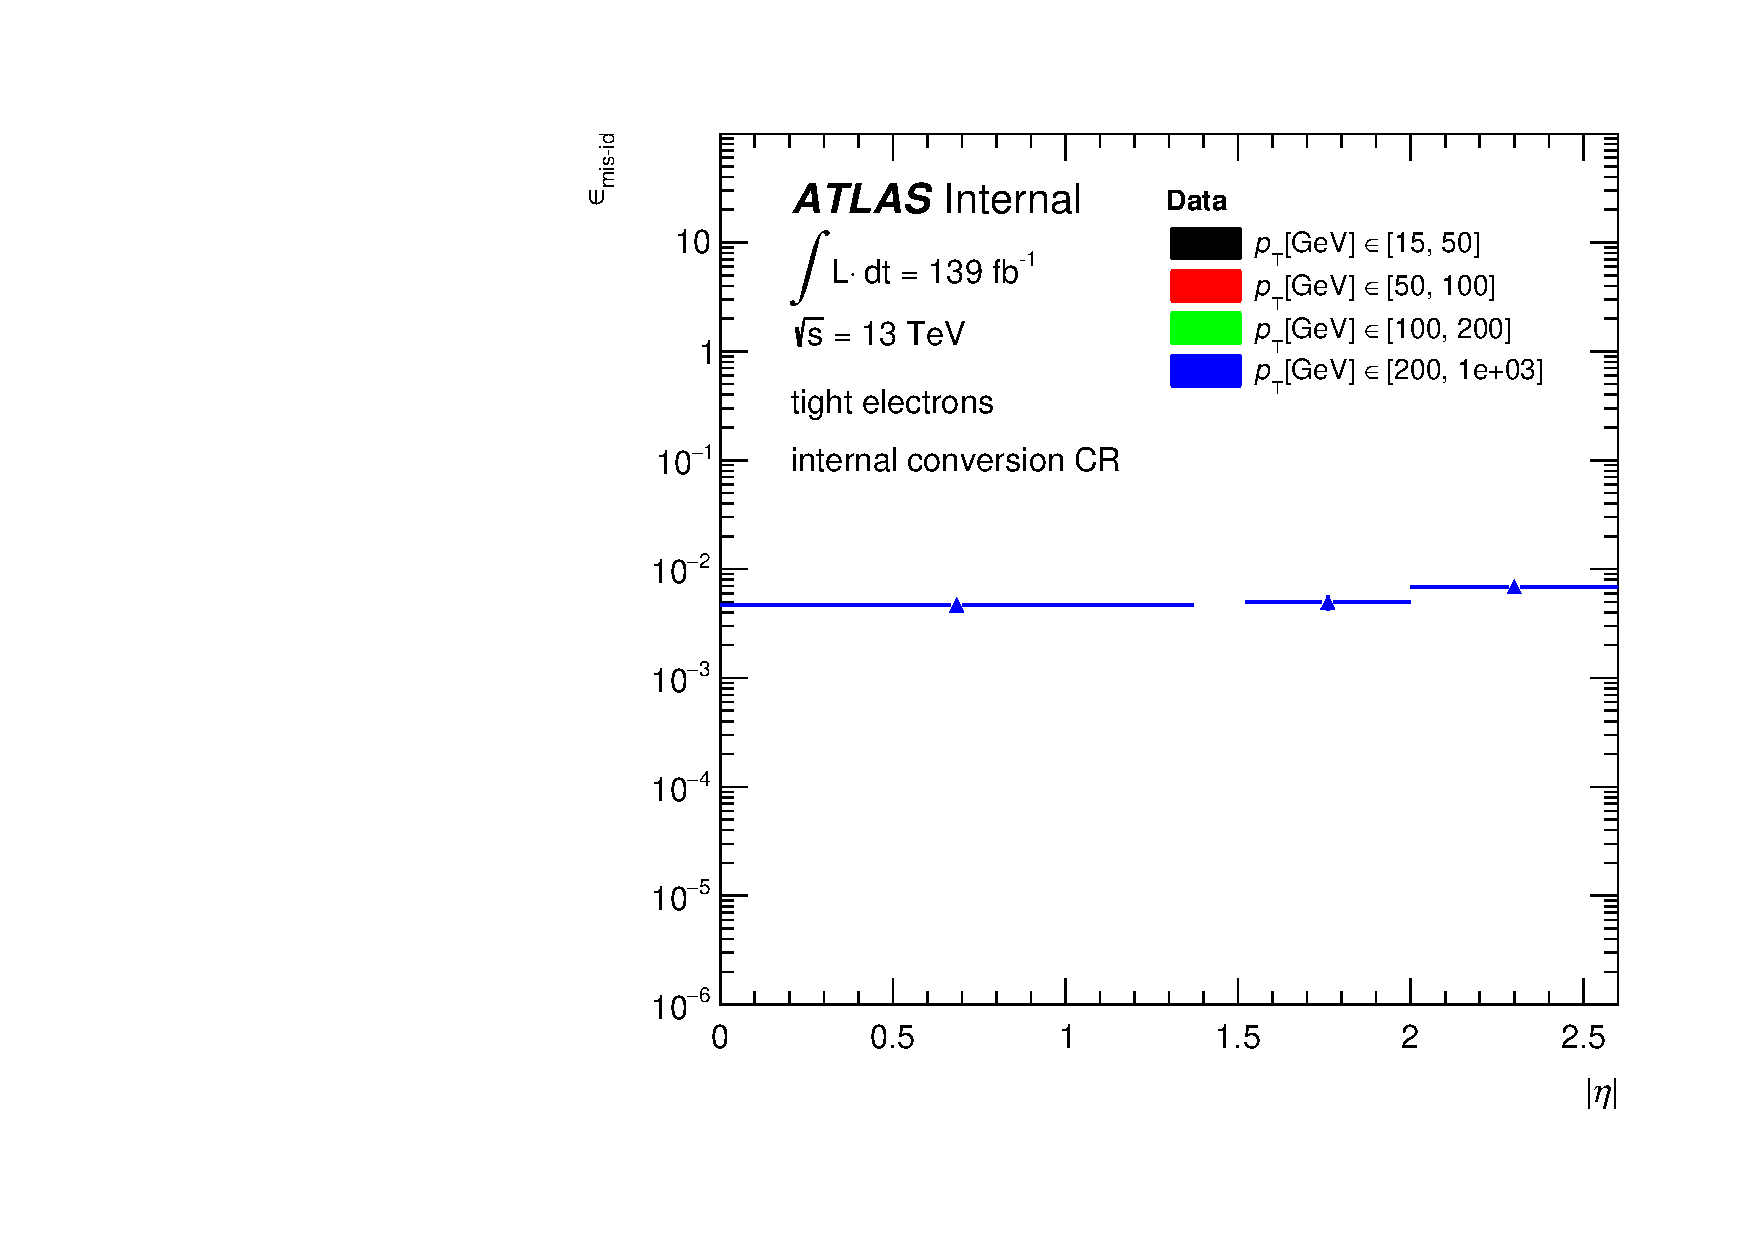
\includegraphics[width=0.32\textwidth]{figures/qmisid/crateData_tight_m0}}
  {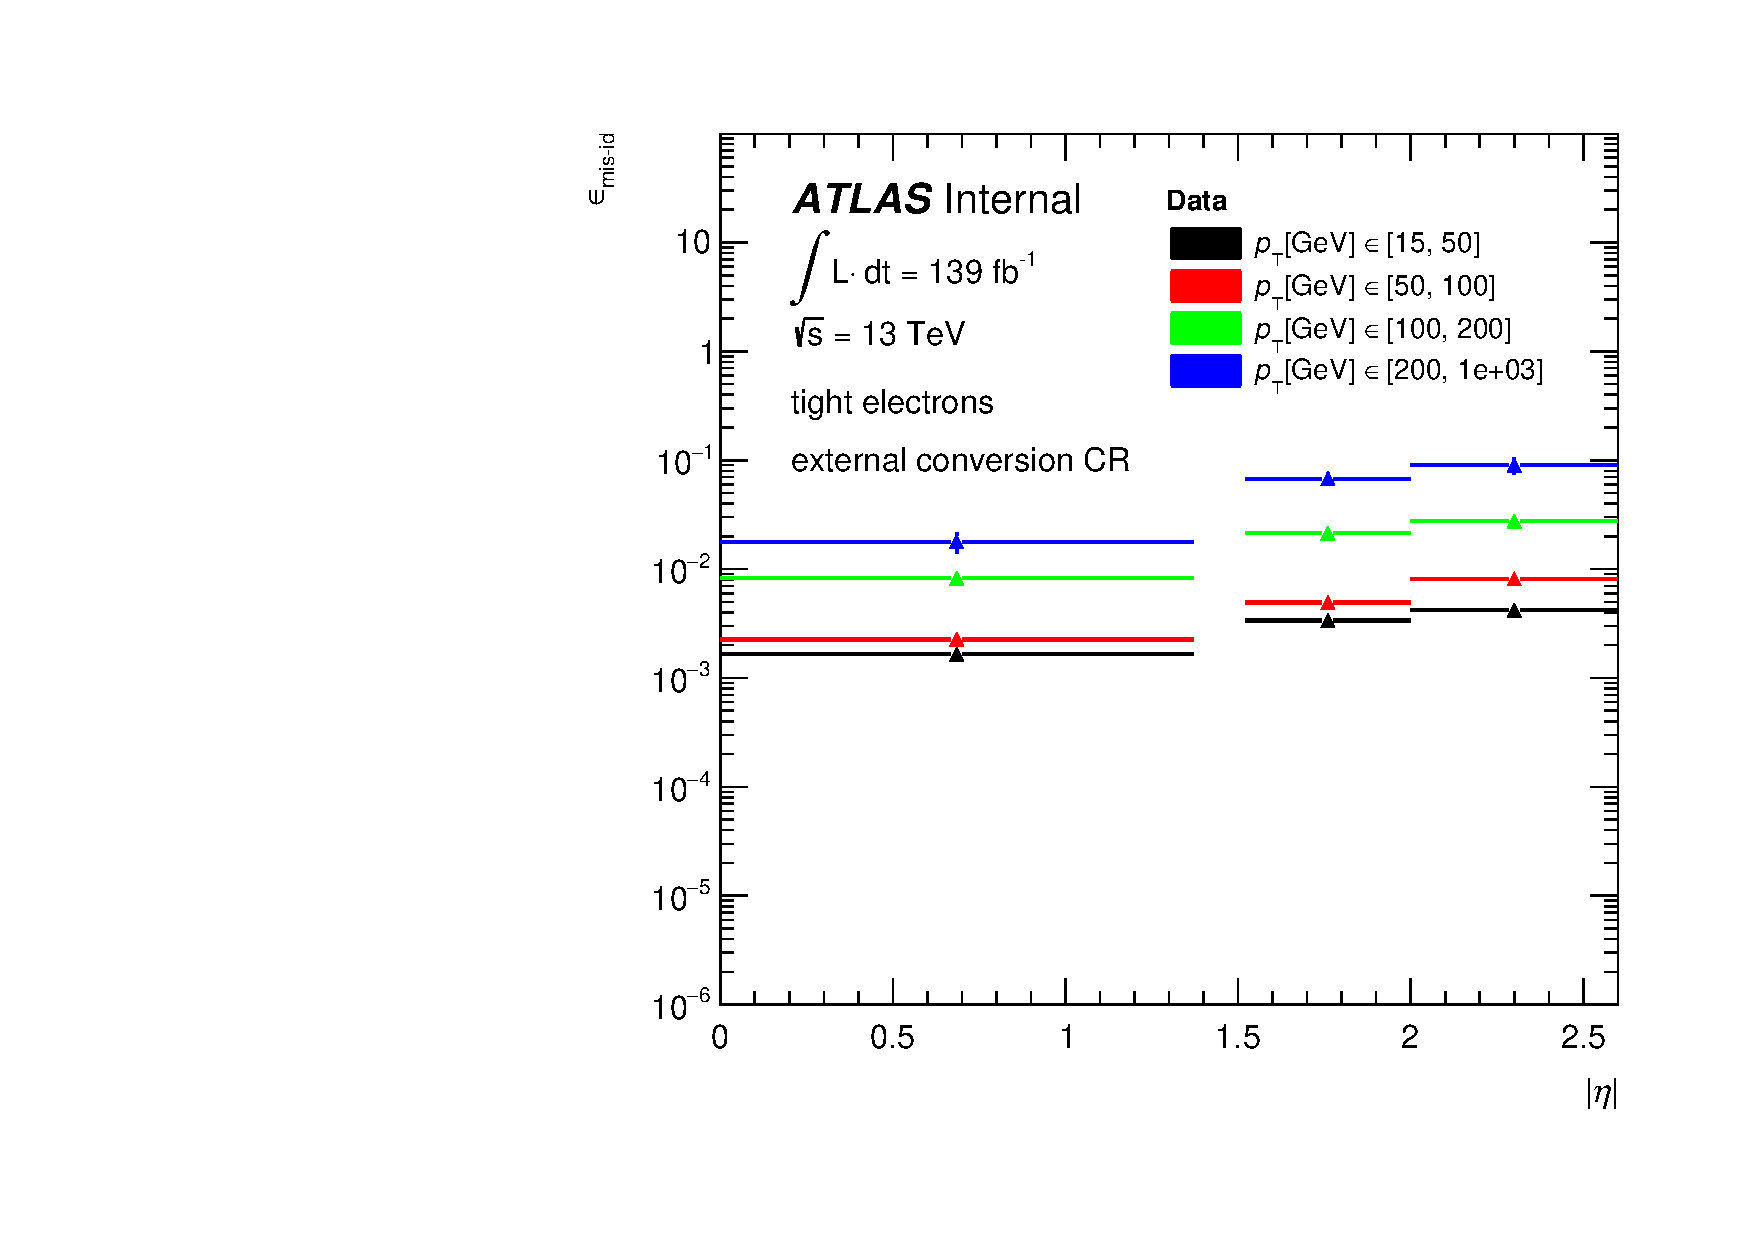
\includegraphics[width=0.32\textwidth]{figures/qmisid/crateData_tight_m1}}
  {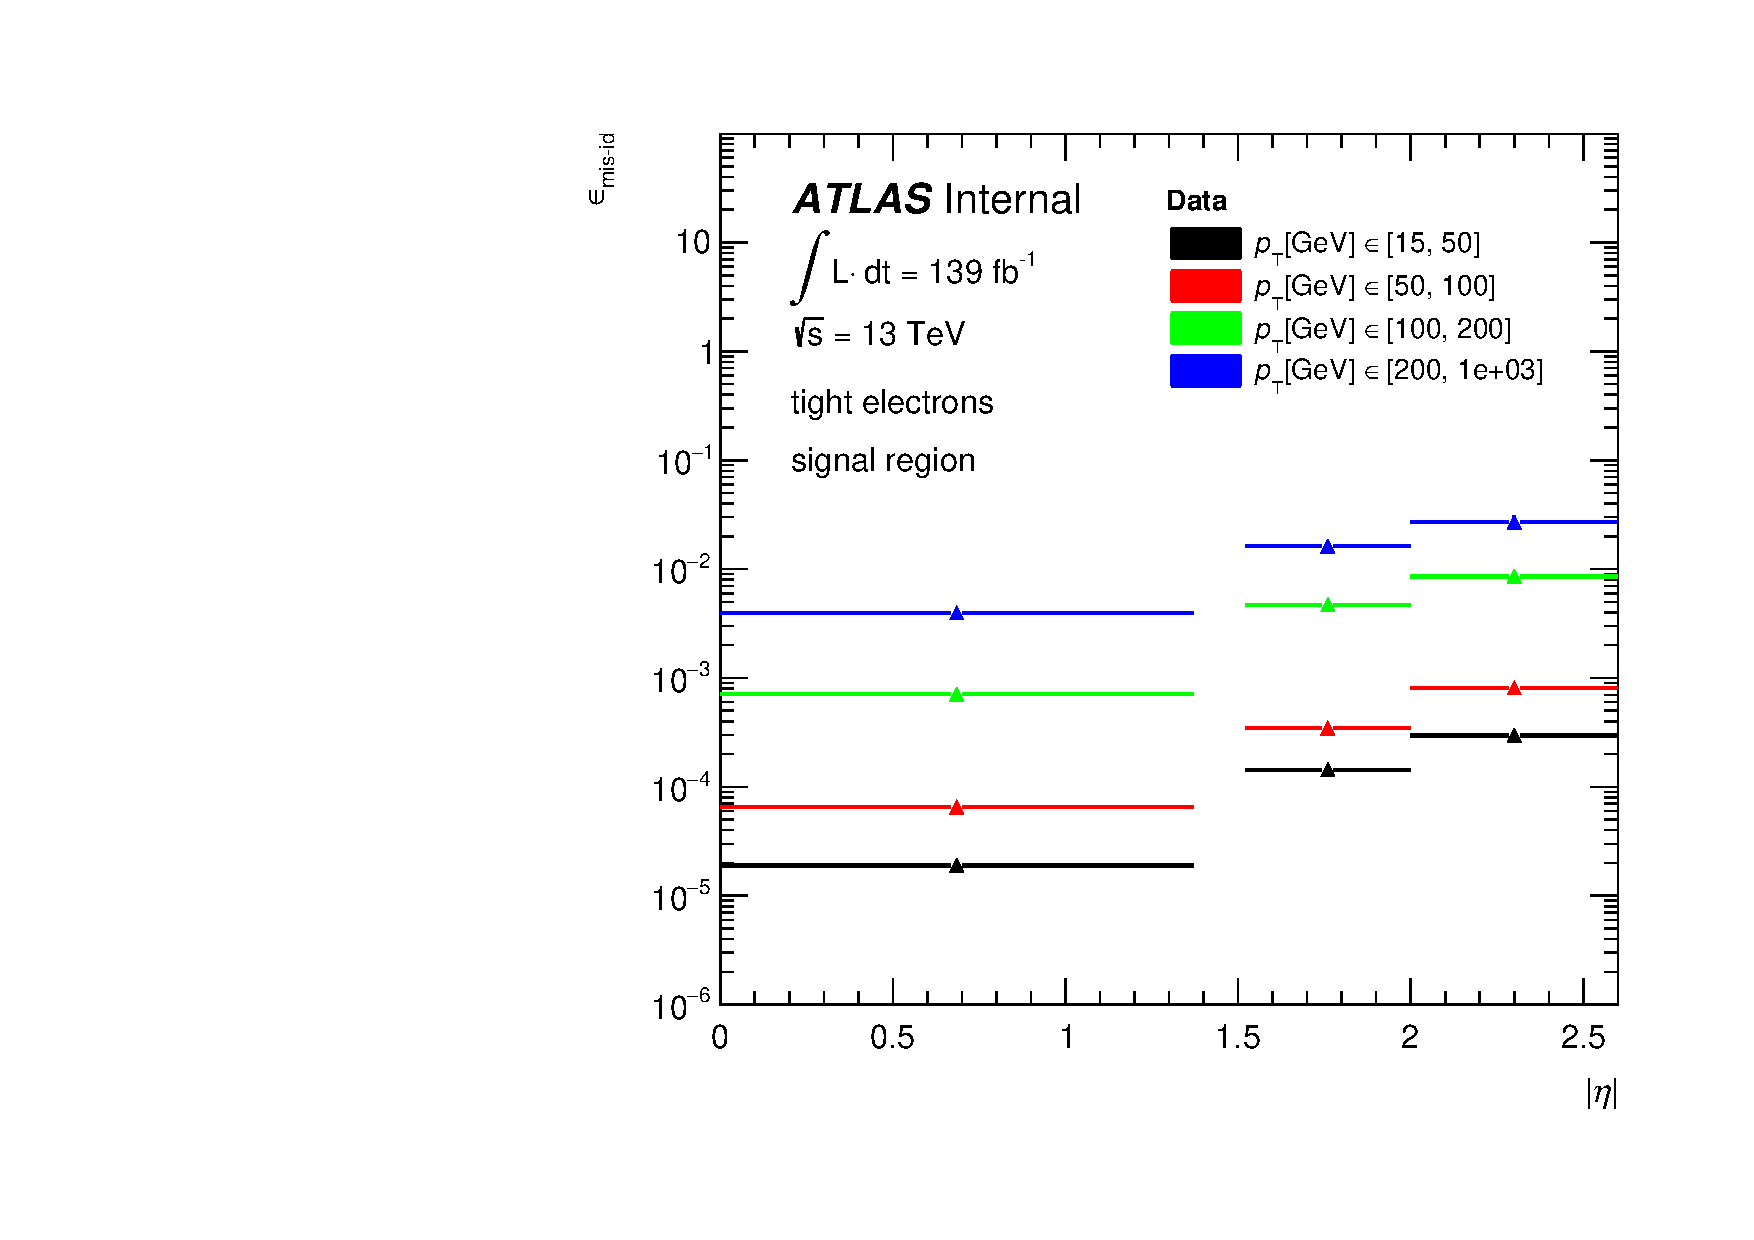
\includegraphics[width=0.32\textwidth]{figures/qmisid/crateData_tight_m2}}
  \caption{Electron charge-flip rates derived from the data with the likelihood method. The rates are presented 
           as a function of $|\eta|$, parameterised in $\pT$ for (a) internal-conversion (b) external-conversion 
           and (c) prompt candidates.\label{fig:Lik2Ddata_main}}
\end{figure}

\begin{figure}[htp!] 
  \centering
  {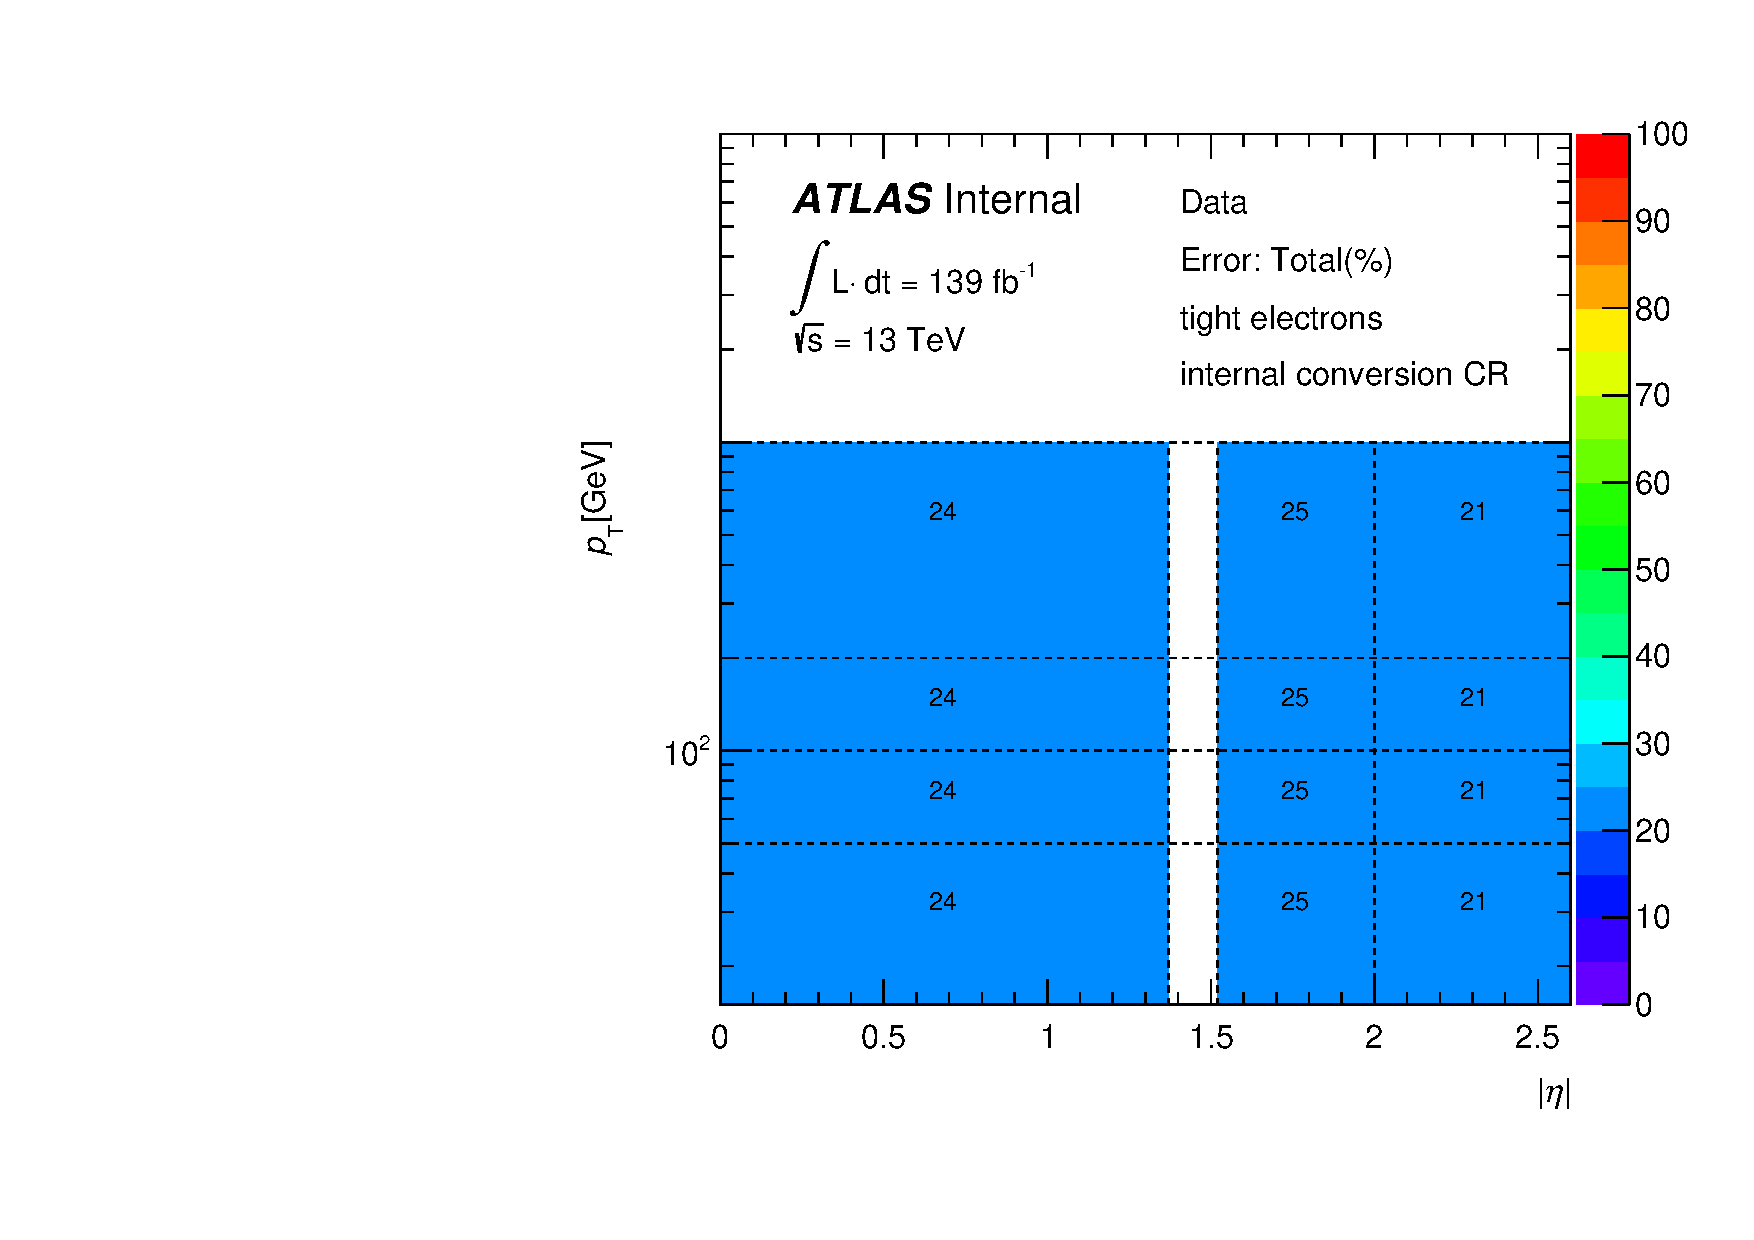
\includegraphics[width=0.32\textwidth]{figures/qmisid/syst_Data_Total_tight_intcr}}
  {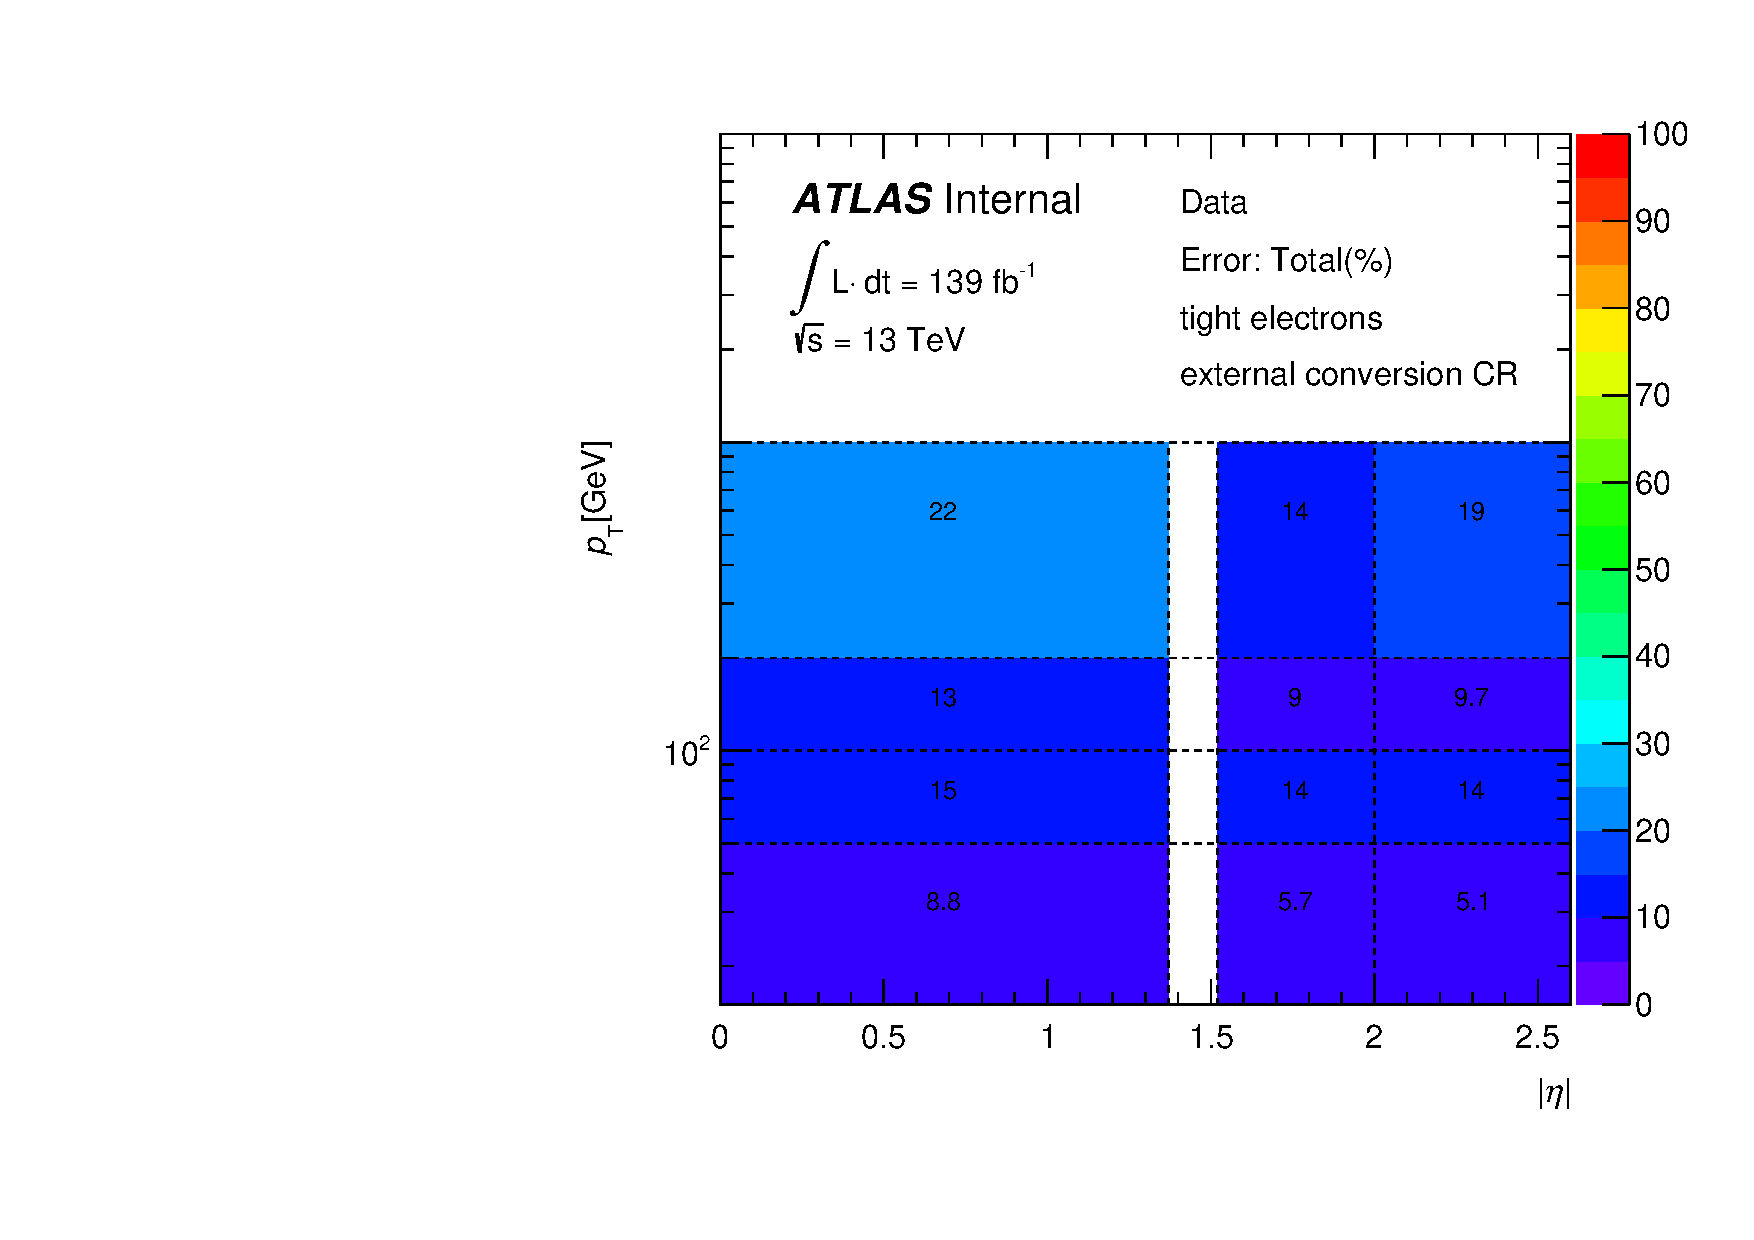
\includegraphics[width=0.32\textwidth]{figures/qmisid/syst_Data_Total_tight_extcr}}
  {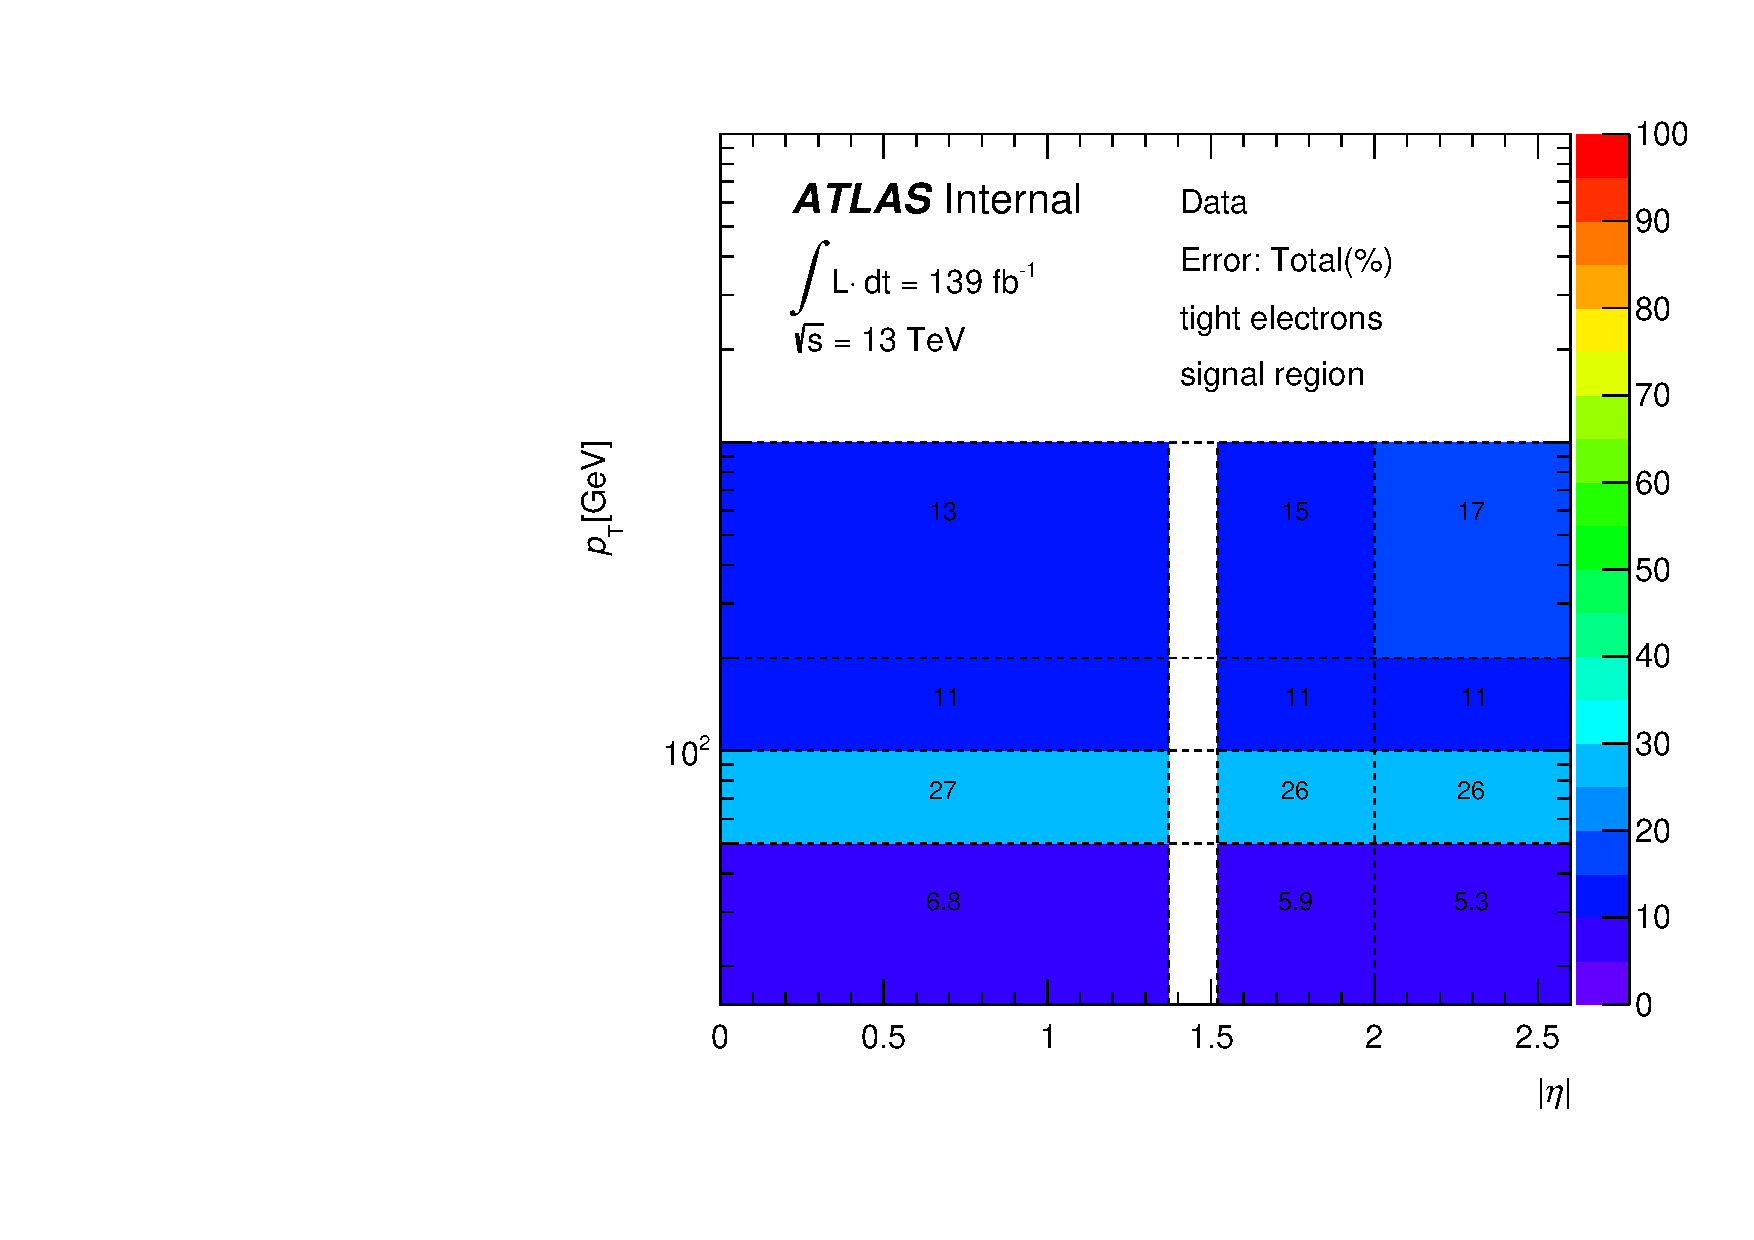
\includegraphics[width=0.32\textwidth]{figures/qmisid/syst_Data_Total_tight_sr}}
  \caption{Total relative systematic uncertainty (in \%) on the charge-flip rate in bins of $|\eta|$ and 
           $\pT$ for (a) internal-conversion (b) external-conversion and (c) prompt electron candidates.
           \label{fig:QMisID:systtight1} }
\end{figure}

Event yields with charge flip electrons are obtained by weighing pre-selected events but asking for 
opposite-sign lepton instead of same-sign. The event weights ($w_{QmisID}$) are defined as:
with the expression:
\begin{equation}
w_{QmisID} = \frac{\epsilon_{\textrm{mis id},1} + \epsilon_{\textrm{mis id},2} - 2\epsilon_{\textrm{mis id},1}\epsilon_{\textrm{mis id},2}}{1-(\epsilon_{\textrm{mis id},1} + \epsilon_{\textrm{mis id},2} - 2\epsilon_{\textrm{mis id},1}\epsilon_{\textrm{mis id},2})}
\label{eq:QmisID_weight}
\end{equation}

where $\epsilon_{\textrm{mis id},1}(1-\epsilon_{\textrm{mis
    id},2})+\epsilon_{\textrm{mis id},2}(1-\epsilon_{\textrm{mis id},1}) =
\epsilon_{\textrm{mis id},1} + \epsilon_{\textrm{mis id},2} -
2\epsilon_{\textrm{mis id},1}\epsilon_{\textrm{mis id},2}$ is the rate of
events in which exactly one electron is reconstructed with charge flip.
In order to account for the strong dependence of the rates to the $\pT$ and to
improve the modeling of the kinematical observables, $\pT$ continuous rates are used.

\subsection{Electron charge flip background study}

The following paragraphs present the measurement of the background, introduced to final states with two 
same-sign light leptons ($e^{\pm}e^{\pm}$, $e^{\pm}\mu^{\pm}$) due to electron charge misidentification 
(QMisID).\footnote{Unless specified otherwise, positrons and electrons are both called electrons.} There 
are two main mechanisms contributing to QMisID:
%
\begin{itemize}
  \item Hard Bremsstrahlung ($e^\pm \rightarrow e^\pm \gamma^* \rightarrow e^\pm e^+e^-$). In this 
  case, QMisID occurs when the EM cluster is coupled to the track of the opposite-sign electron 
  in the trident. Since the probability of this process depends on the traversed detector material, 
  dependence of the QMisID rate on $|\eta|$ is expected.
  \item Mismeasurement of the electron track-curvature. This effect is more important in the high 
  $p_{\mathrm T}$ range (smaller curvature), therefore dependence of the rate on $p_{\mathrm T}$ 
  is also expected.
\end{itemize}
%
The misidentification of the muon charge-sign is not considered in this study. It may occur by mismeasurement 
of the track curvature, however, due to the long lever arm in the muon system and the fact that the charge is 
measured both in the inner detector and the muon spectrometer, the QMisID rate is marginal.

The estimation of the QMisID background is based on the electron QMisID rates $\vec{\epsilon}$. The latter 
are derived from the data, in three-dimensional (3D) bins according to $|\eta|$, $p_{\mathrm T}$ and the 
region to which the electron belongs with respect to photon conversions, i.e. it designated as internal- 
or external-conversion candidate or as prompt lepton (as defined in the
same-sign signal region).



%~~~~~~~~~~~~~~~~~~~~~~~~~~~~~~~~~~~
\subsubsection{Background estimation strategy} 
%~~~~~~~~~~~~~~~~~~~~~~~~~~~~~~~~~~~
Final states with an opposite-sign lepton pair (mainly $Z \rightarrow e^+e^- $
followed by $t\bar{t} \rightarrow b\bar{b}W^+W^- \rightarrow b\bar{b}e^+e^-\nu\bar{\nu}$)
contaminate the signal region, defined by two same-sign leptons, when the charge of exactly one lepton
is misidentified. In the case of $e^{-}e^{+}$, the fraction of events that are reconstructed as same-sign 
($e^{-}e^{-}$ or $e^{+}e^{+}$) is:
%
\begin{equation}
  \epsilon_i(1-\epsilon_j) + \epsilon_j(1-\epsilon_i) = \epsilon_i +\epsilon_j - 2\epsilon_i\epsilon_j, 
\end{equation}
%
where $\epsilon_i$ and $\epsilon_j$ are the QMisID rates for each of the two electrons. For $e^{\pm}\mu^{\mp}$ 
events, on the other hand, the respective fraction is equal to the QMisID rate $\epsilon_i$ of the electron. 
By knowing the QMisID rates it is thereby possible to compute the expected number of misidentified same-sign 
events $\bar{N}_\mathrm{SS}$ from the observed number of opposite-sign events $N_\mathrm{OS}$, using the expressions:
%
\begin{equation}
  \bar{N}_\mathrm{SS} = \frac{\epsilon_i +\epsilon_j -2\epsilon_i \epsilon_j}{1-(\epsilon_i +\epsilon_j -2\epsilon_i \epsilon_j)} N_\mathrm{OS}
  \hspace{10pt}\text{and}\hspace{10pt}
  \bar{N}_\mathrm{SS} = \frac{\epsilon_i}{1-\epsilon_i} N_\mathrm{OS}
\end{equation}
%
for the $ee$ and $e\mu$ channel, respectively.

%~~~~~~~~~~~~~~~~~~~~~~~~~~~~~~~~~~~
\subsubsection{Estimation of the charge mis-identification rates with the likelihood method} 
%~~~~~~~~~~~~~~~~~~~~~~~~~~~~~~~~~~~
The QMisID rates are derived from the data, based on the fraction of $Z\rightarrow ee$ decays that are reconstructed 
as a same-sign electron pair. For this measurement, events in the $m_{ee}$ region around the reconstructed $Z$-boson 
peak $m_Z$ are used. For $N^{ij}$ electron pairs falling in the bin combination $i,j$ (where each of $i,j$ uniquely 
represents a 3D bin as defined above) the expected number of same-sign events is:
%
\begin{equation}
  \label{app:eq:qmisid1}
  \bar{N}^{ij}_\mathrm{SS}(\epsilon_i,\epsilon_j)=N^{ij}\cdot(\epsilon_i+\epsilon_j-2\epsilon_i\epsilon_j).
\end{equation}
%
Asumming that all of the observed same-sign events, $N^{ij}_\mathrm{SS}$, in the $m_Z$ window are products 
of electron charge mis-identification, they follow a Poisson distribution around the expectation value:
%
\begin{equation}
\label{app:eq:qmisid2}
  f(N^{ij}_\mathrm{SS}|\bar{N}_\mathrm{SS}(\epsilon_i,\epsilon_j))=\frac{[{\bar{N}}^{ij}_\mathrm{SS}]^{N^{ij}_\mathrm{SS}} e^{-{\bar{N}}^{ij}_\mathrm{SS}}}{N^{ij}_\mathrm{SS}!}.
\end{equation}

which is integrated into a likelihood:
%
\begin{equation}
  L(\vec{\epsilon}|N_\mathrm{SS})=\prod_{i,j}f(N^{ij}_\mathrm{SS}|\bar{N}_\mathrm{SS}(\epsilon_i,\epsilon_j)).
\end{equation}
%
that can be maximised (minimisation of $-2\ln L$) to obtain the rates that best describe the data. 

As mentioned above, this method relies on the assumption that $ee$ events in the $m_Z$ window are products of $Z$-boson decays. 
Therefore, any contribution from other processes (e.g. fake electrons) to $N^{ij}_\mathrm{SS}$ must be subtracted. As long as 
these processes do not exhibit a resonant-like behaviour of the $m_{ee}$ distribution, this background can be estimated from 
the sidebands of the $m_{Z}$ window, for each bin combination $i,j$, separately for same-sign ($N^{ij}_\mathrm{SS,BG}$) and 
opposite-sign ($N^{ij}_\mathrm{OS,BG}$) events. For this, upper and lower sidebands are defined with width equal to the $m_{Z}$ 
window so that the introduced background can be obtained from the average yield. The background estimate is then used to correct 
the expectation (equation\,\ref{app:eq:qmisid1}) to:
%
\begin{equation}
  \bar{N}^{ij}_\mathrm{SS} = N^{ij}_\mathrm{SS,BG} + (N^{ij}-N^{ij}_\mathrm{SS,BG}-N^{ij}_\mathrm{OS,BG})\cdot(\epsilon_i+\epsilon_j-2\epsilon_i\epsilon_j).
\end{equation}
%
The minimisation of $-2\ln L$ is finally performed by MIGRAD, while HESSE is called to evaluate the uncertainty on the 
rate estimates. 

%~~~~~~~~~~~~~~~~~~~~~~~~~~~~~~~~~~~
\subsubsection{Data and Monte Carlo samples}
\label{sec:qmisiddata}
%~~~~~~~~~~~~~~~~~~~~~~~~~~~~~~~~~~~

The QMisID rate and background estimation is performed using the full dataset, with an integrated luminosity 
of 139\,fb$^{-1}$. For the validation of the method and many of the tests that follow, 
simulated $Z\to ee$ ({\scshape Sherpa}), $t\bar{t}$ (\textsc{Powheg-BOX}) and $t\bar{t}\gamma$ (\textsc{MG5\_aMC}) samples 
are also used.

No additional criteria are applied to electrons for the QMisID rate
estimation. In order to increase the size of the tight electron sample,
anti-tight electrons are also exploited.  
The latter are defined as those electrons that fail the tight identification criteria but yet pass the overlap removal. Although such 
electrons are not used in the analysis, by using a looser set of electrons and classifying them as tight and anti-tight (on top of the 
3D classification described above), introduces events with one tight and one anti-tight electron in the rate estimation, and therefore 
improves the statistical precision of the tight-electron rates with the likelihood method.

%~~~~~~~~~~~~~~~~~~~~~~~~~~~~~~~~~~~~~~~~~~~~~~~~~~~~~~~~~~~~~~~~~~~~~~~~~~
\subsubsection{$M_{ee}$ sidebands for $Z\rightarrow ee$ background estimation}
\label{app:sec:AppQMisIDregions}
%~~~~~~~~~~~~~~~~~~~~~~~~~~~~~~~~~~~~~~~~~~~~~~~~~~~~~~~~~~~~~~~~~~~~~~~~~~

The likelihood method uses $Z\rightarrow ee$ decays with both same-sign and opposite-sign electrons in the final state. As shown 
in figure\,\ref{fig:mlldata}, the $m_{ee}$ distribution of same-sign electrons is shifted towards lower values with respect to 
that of opposite-sign electrons, due to the loss of electron momentum in tridents. To account for this shift, a different $m_Z$ 
window is defined for each case. The $m_Z$ window is determined by gaussian fit around the peak (using all loose electrons) and 
defined as $\pm 4\sigma$ around the mean ($4\sigma$ has been found to provide the best results in terms of closure). The side-bands 
are defined with equal width to the $m_Z$ window, i.e. $8\sigma$ each. The region definitions are summarised in table~\ref{tab:QMisID:Ranges}.
The variation of the rates with the definition of the $m_Z$ window ($\pm 1\sigma$) is considered as a systematic uncertainty.

\smallskip

\begin{table}[h!]
  \begin{center}
    \begin{tabular}{l c c c}
      Sample & lower SB & $m_Z$ window & upper SB \\
      Same-sign & [51.7,76.5] & [76.5,101.3] & [101.3,126.0] \\
      Opposite-sign & [54.7,78.5] & [78.5,102.3] & [102.3,126.0] \\
    \end{tabular}
     \caption{Definition of the $m_Z$ window and side-bands (SB) used in the likelihood method.\label{tab:QMisID:Ranges}}
  \end{center}
\vspace*{-\baselineskip}
\end{table}

\begin{figure}[h!]
  \centering
  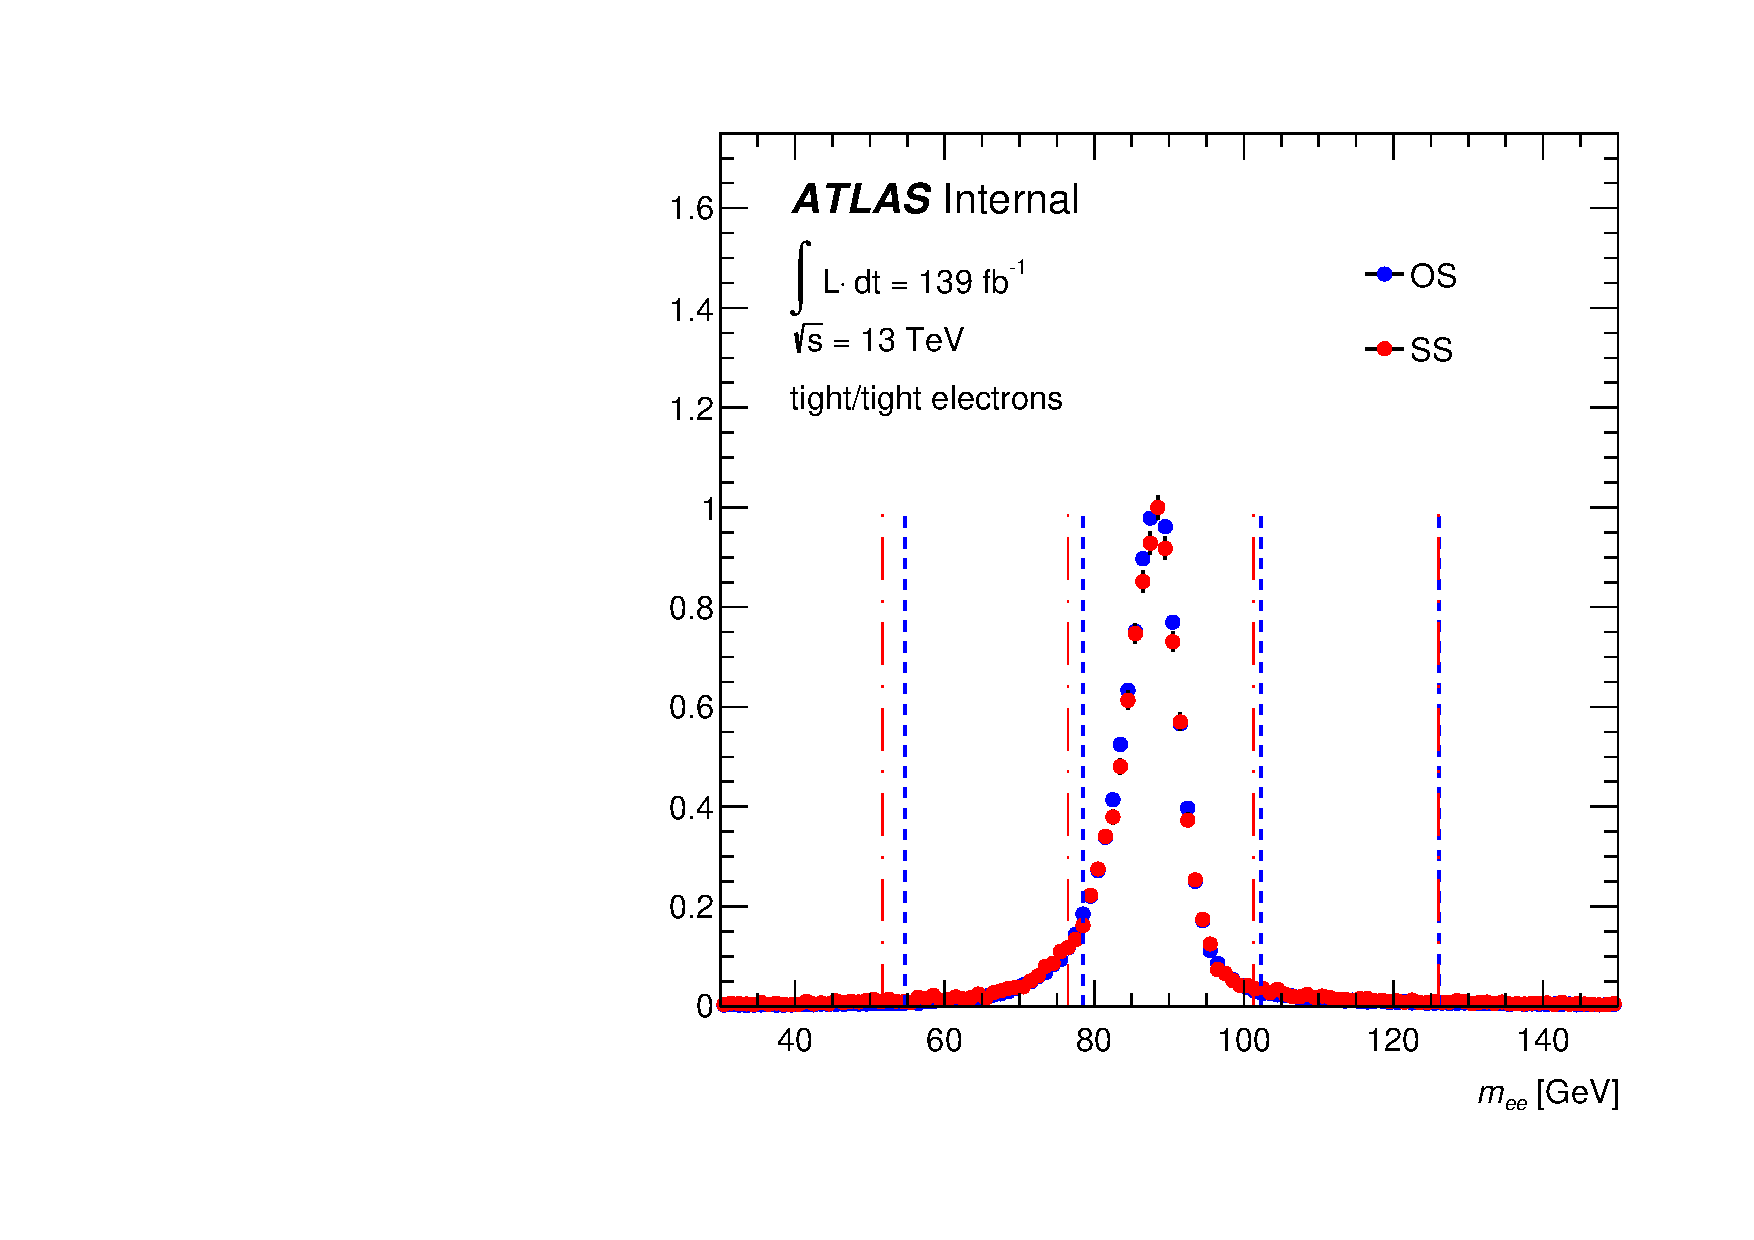
\includegraphics[width=0.45\textwidth]{figures/qmisid/mll_tt}
  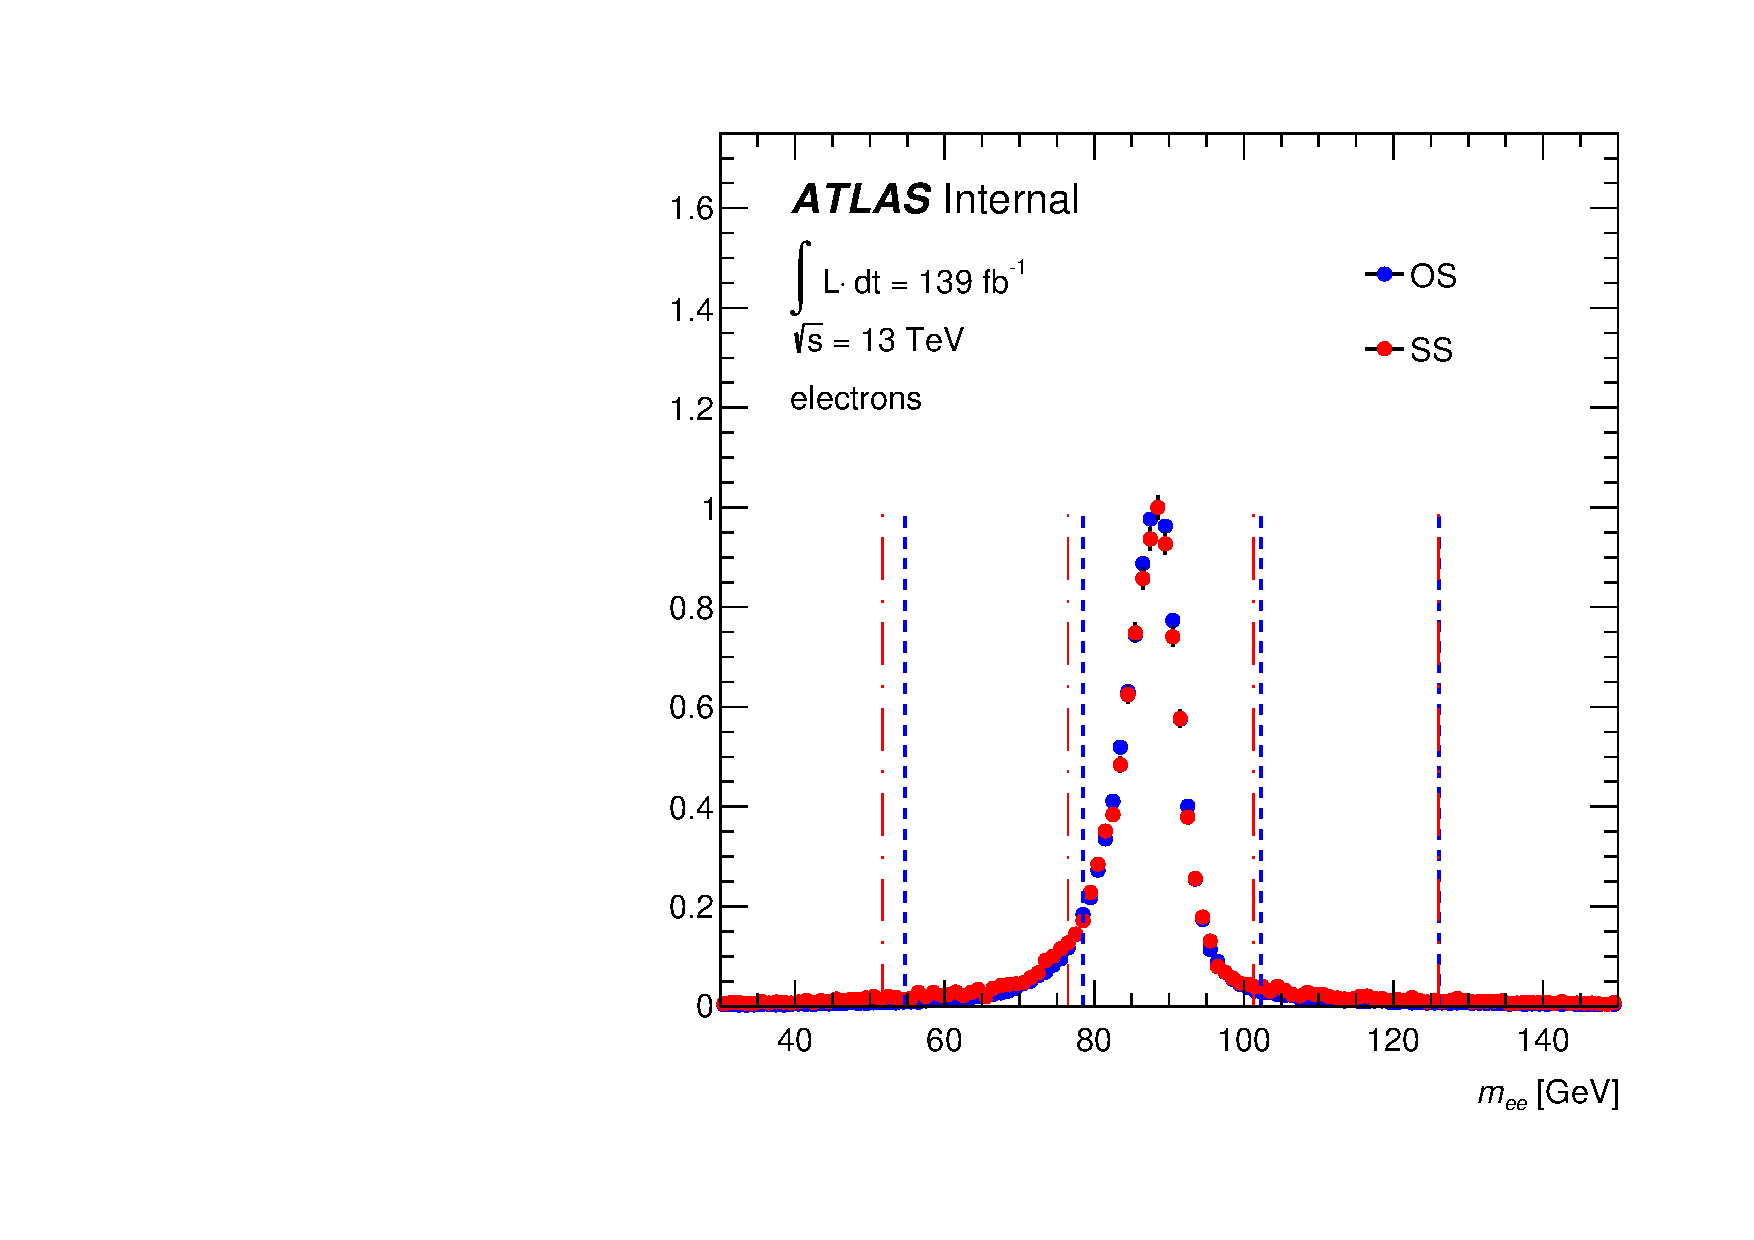
\includegraphics[width=0.45\textwidth]{figures/qmisid/mll_all}
  \caption{Comparison of the $m_{ee}$ distribution between same-sign and opposite-sign data events for pairs of 
  (a) tight and (b) loose electrons. The distributions are 
  normalized by the maximum value. The peak for same-sign electrons is shifted with respect to opposite-sign 
  electrons due to the loss of electron momentum in tridents.\label{fig:mlldata}}
\end{figure}

%~~~~~~~~~~~~~~~~~~~~~~~~~~~~~~~~~~~~~~~~~~~~~~~~~~~~~~~~~~~~~~~~~
\subsubsection{Data-driven rates estimates with $\pT$ continuous rates}
%~~~~~~~~~~~~~~~~~~~~~~~~~~~~~~~~~~~~~~~~~~~~~~~~~~~~~~~~~~~~~~~~~

The binning in $|\eta|$ and $\pT$ must be optimised to best describe the dependence of the rates on each quantity
while maintaing statistical precision.

The binning scheme 
distinguishes four bins in $|\eta|$ 
(one of which just isolates the crack region) and four bins in $\pT$, for each region w.r.t. to photon conversions. 
To mitigate the statistical uncertainties introduced by the size of the available dataset in the case of 
tight-electrons, $\pT$ bins are merged in the case of the internal conversion control region (merging is 
implemented by assigning the same rate in the likelihood).
The data-driven QMisID rates, derived with the above binning configuration, are presented in figure\,\ref{fig:Lik2Ddata}.

Figure\,\ref{fig:DatapTJumps}(a) shows the expected $\pT$ distribution in the
data, using reweighted opposite-sign events, compared to the
observation. Significant non closures are observed at the edges of the $\pT$
bins. These non-closures are covered by the non-closure systematic
uncertainties in average only. The local non-closures exceed significantly the
systematic uncertainties. They can of $200\%$ in the 60-80~GeV range, and higher
than $200\%$ in the 150-200~GeV ranges.
 
In order to control this effect, $\pT$ continuous modeling of the rates is
used. The effective rate at a given $\pT$ is obtained by the weighted
sum of the rates from the adjacend $\pT$ bins. The weighting is based on
$\pT$ only and accounts for the $\pT$ disctribution shape.

\begin{figure}[htb!]
\centering
  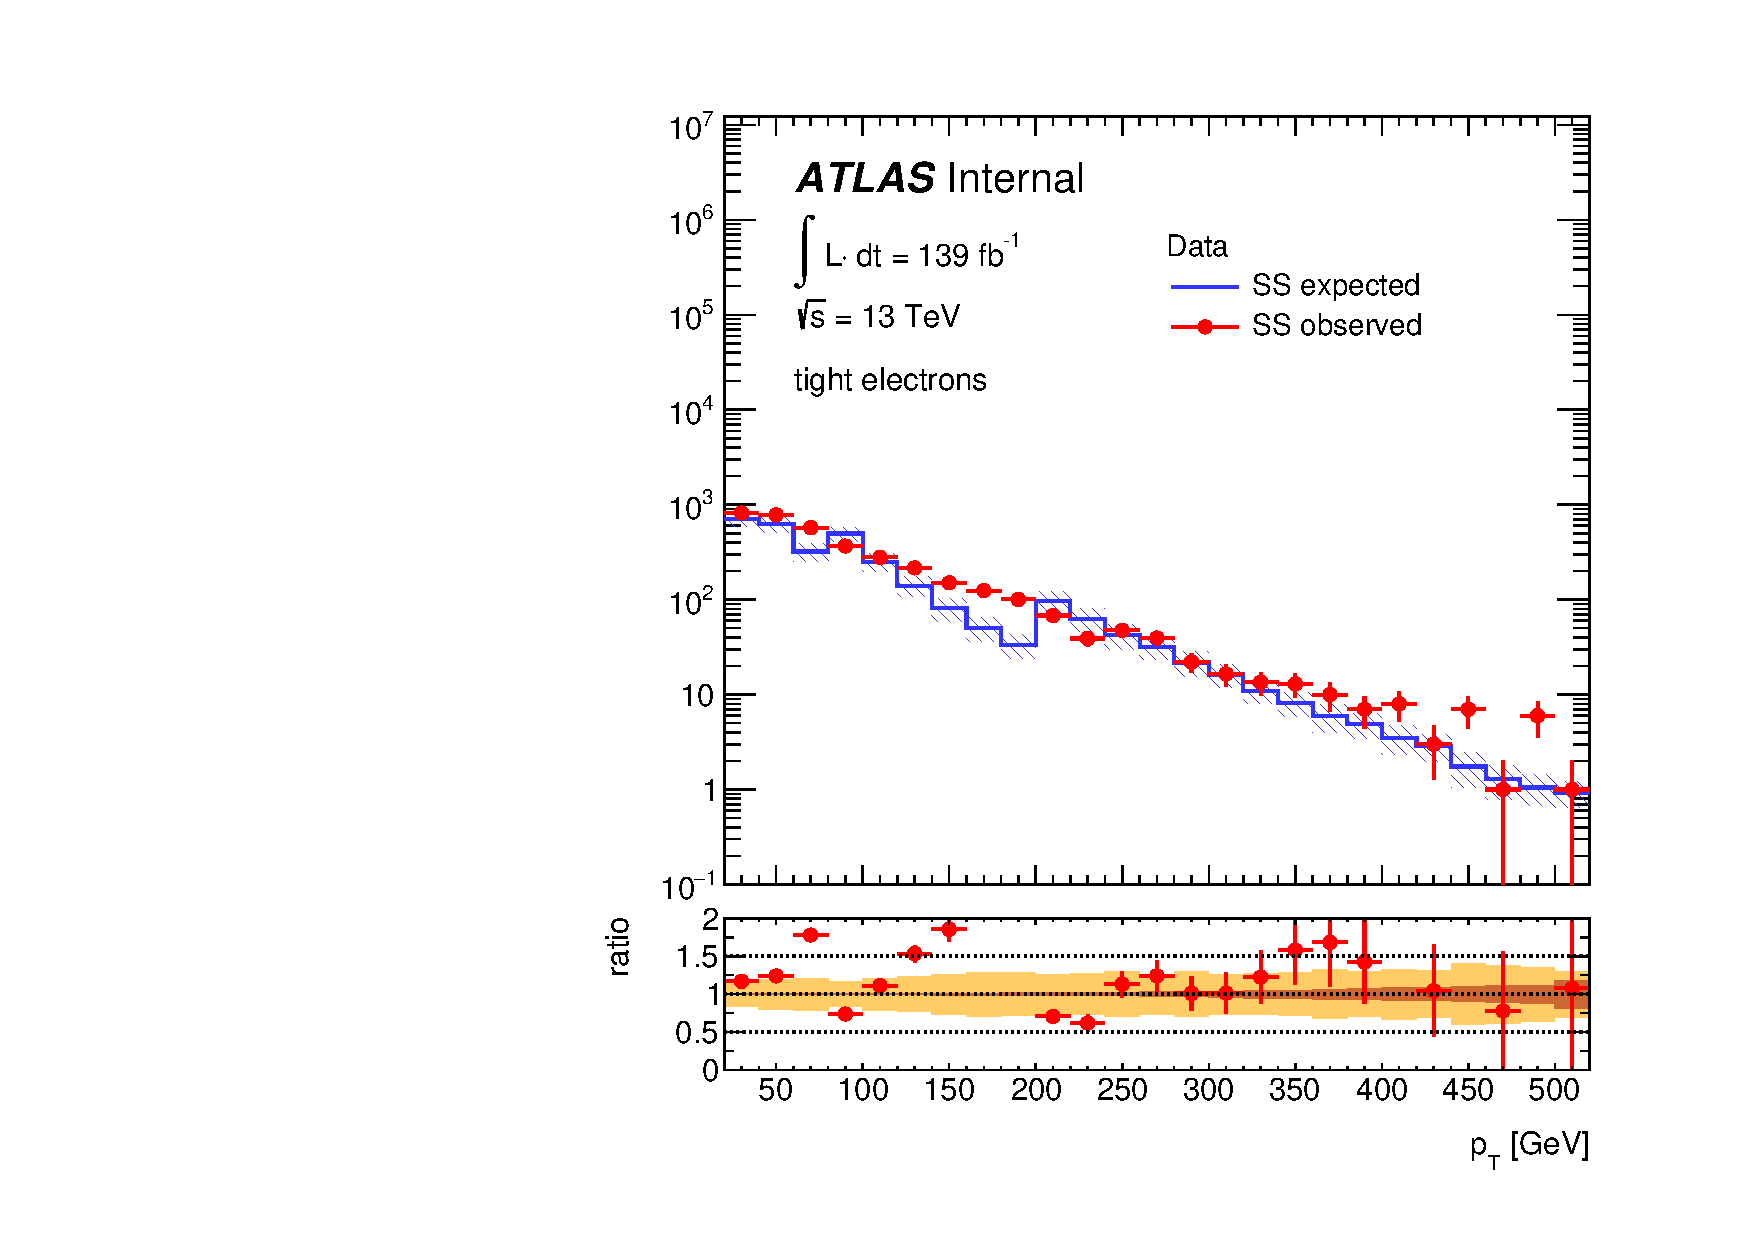
\includegraphics[width=0.45\textwidth]{figures/qmisid/valid_PttightData_binned}
  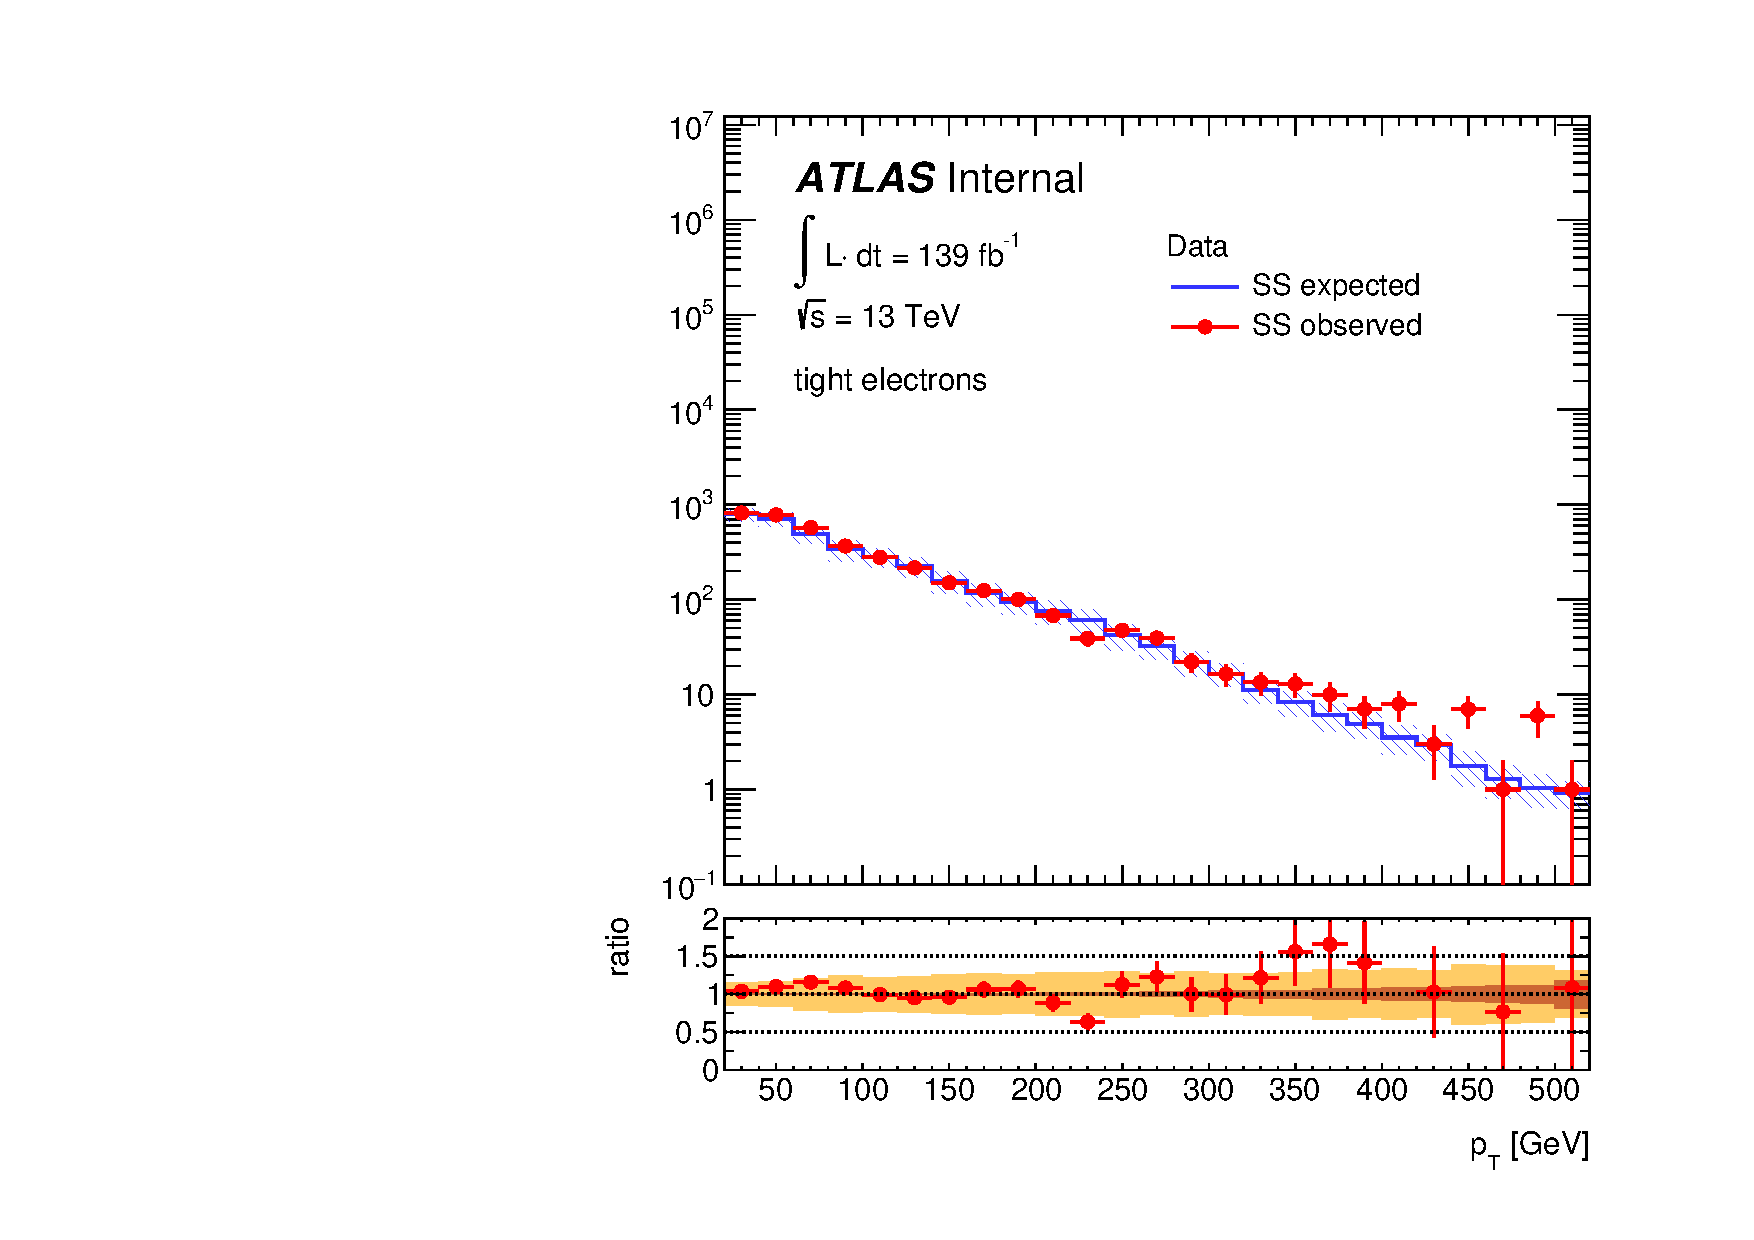
\includegraphics[width=0.45\textwidth]{figures/qmisid/valid_PttightData}\\
  \caption{Comparison between the expected and observed $\pT$ distribution of same-sign electrons.
  The dashed bands represent the total (statistical + systematic) uncertainty of the estimation. The comparison is shown for
  data events. The rates used to compute the predicted distribution are
  binned in $\pT$ (left) or continuous in $\pT$ (right).\label{fig:DatapTJumps}}
\end{figure}


\begin{figure}[tb!]
  \centering
  {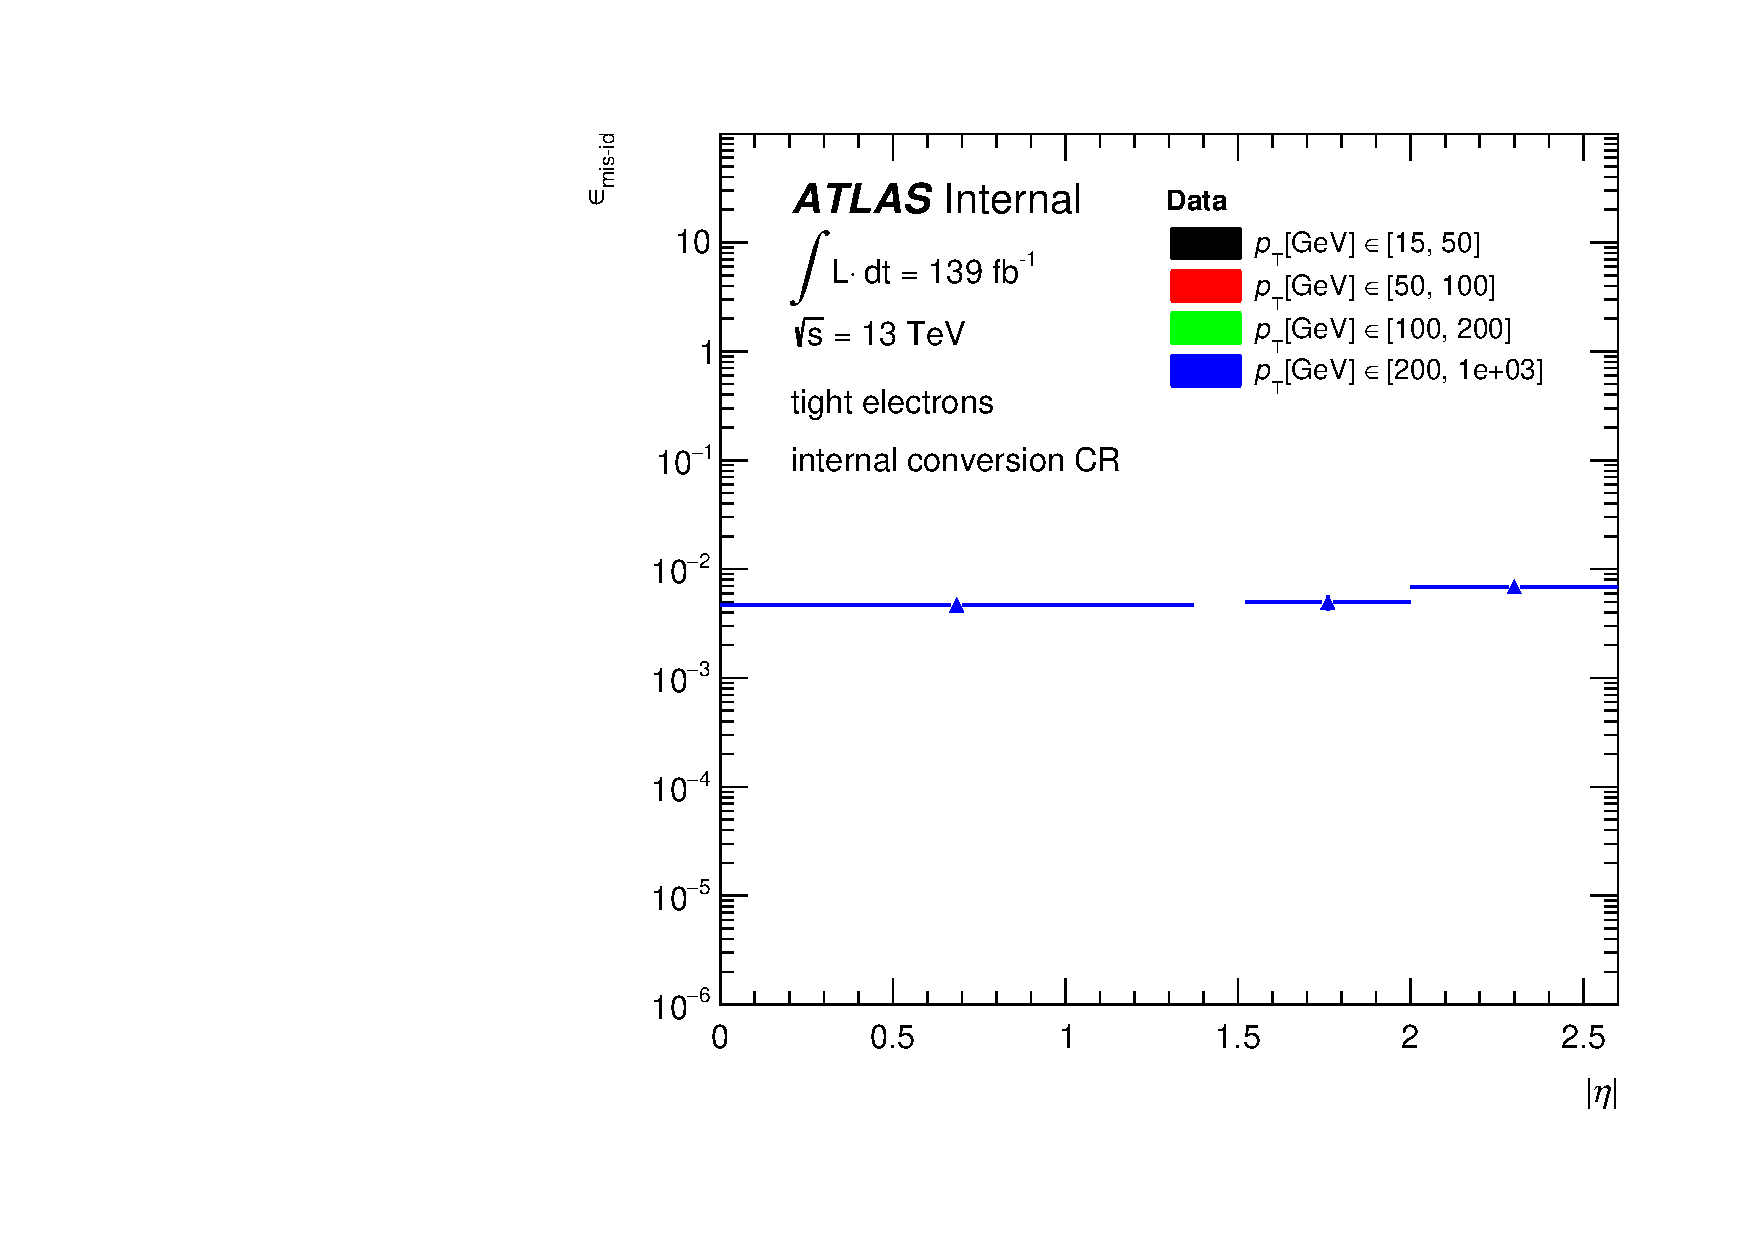
\includegraphics[width=0.37\textwidth]{figures/qmisid/crateData_tight_m0}}
  {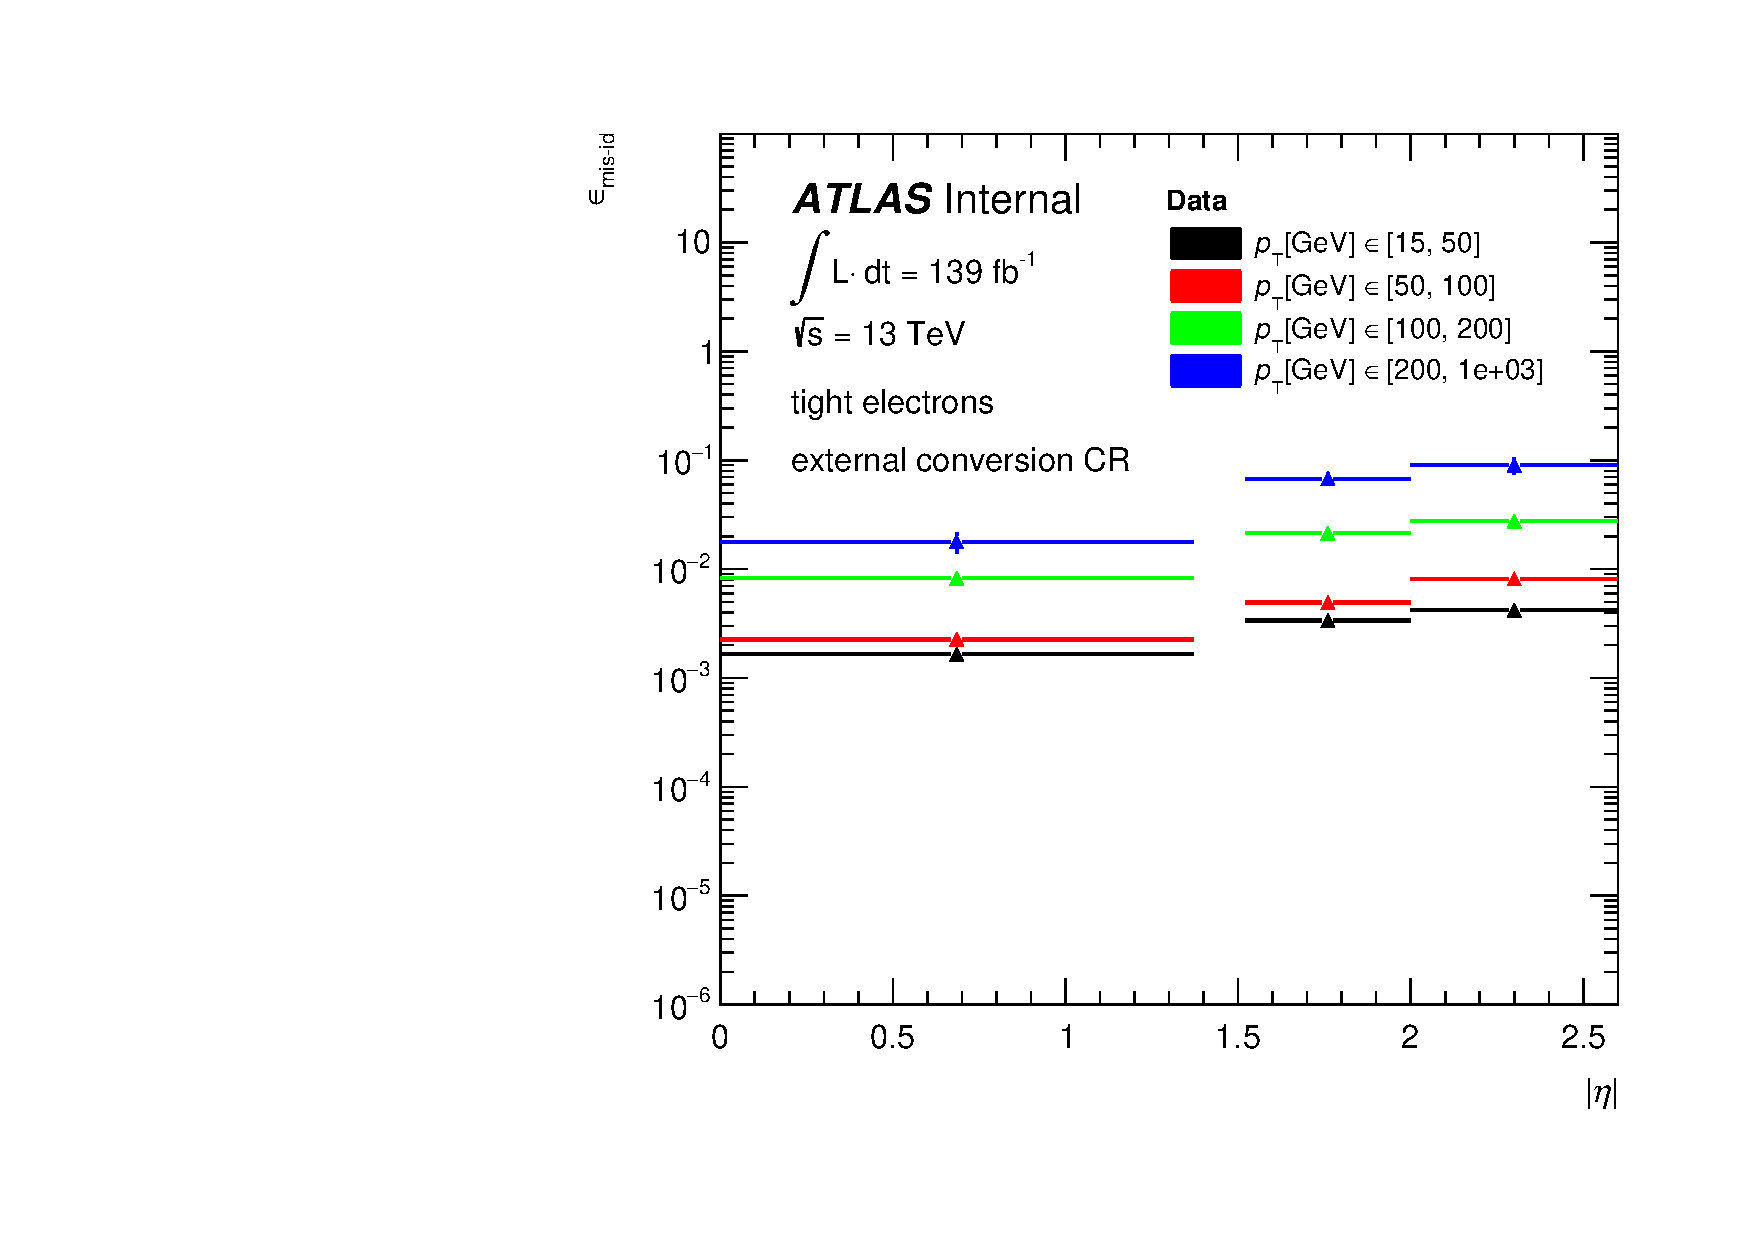
\includegraphics[width=0.37\textwidth]{figures/qmisid/crateData_tight_m1}}\\
  {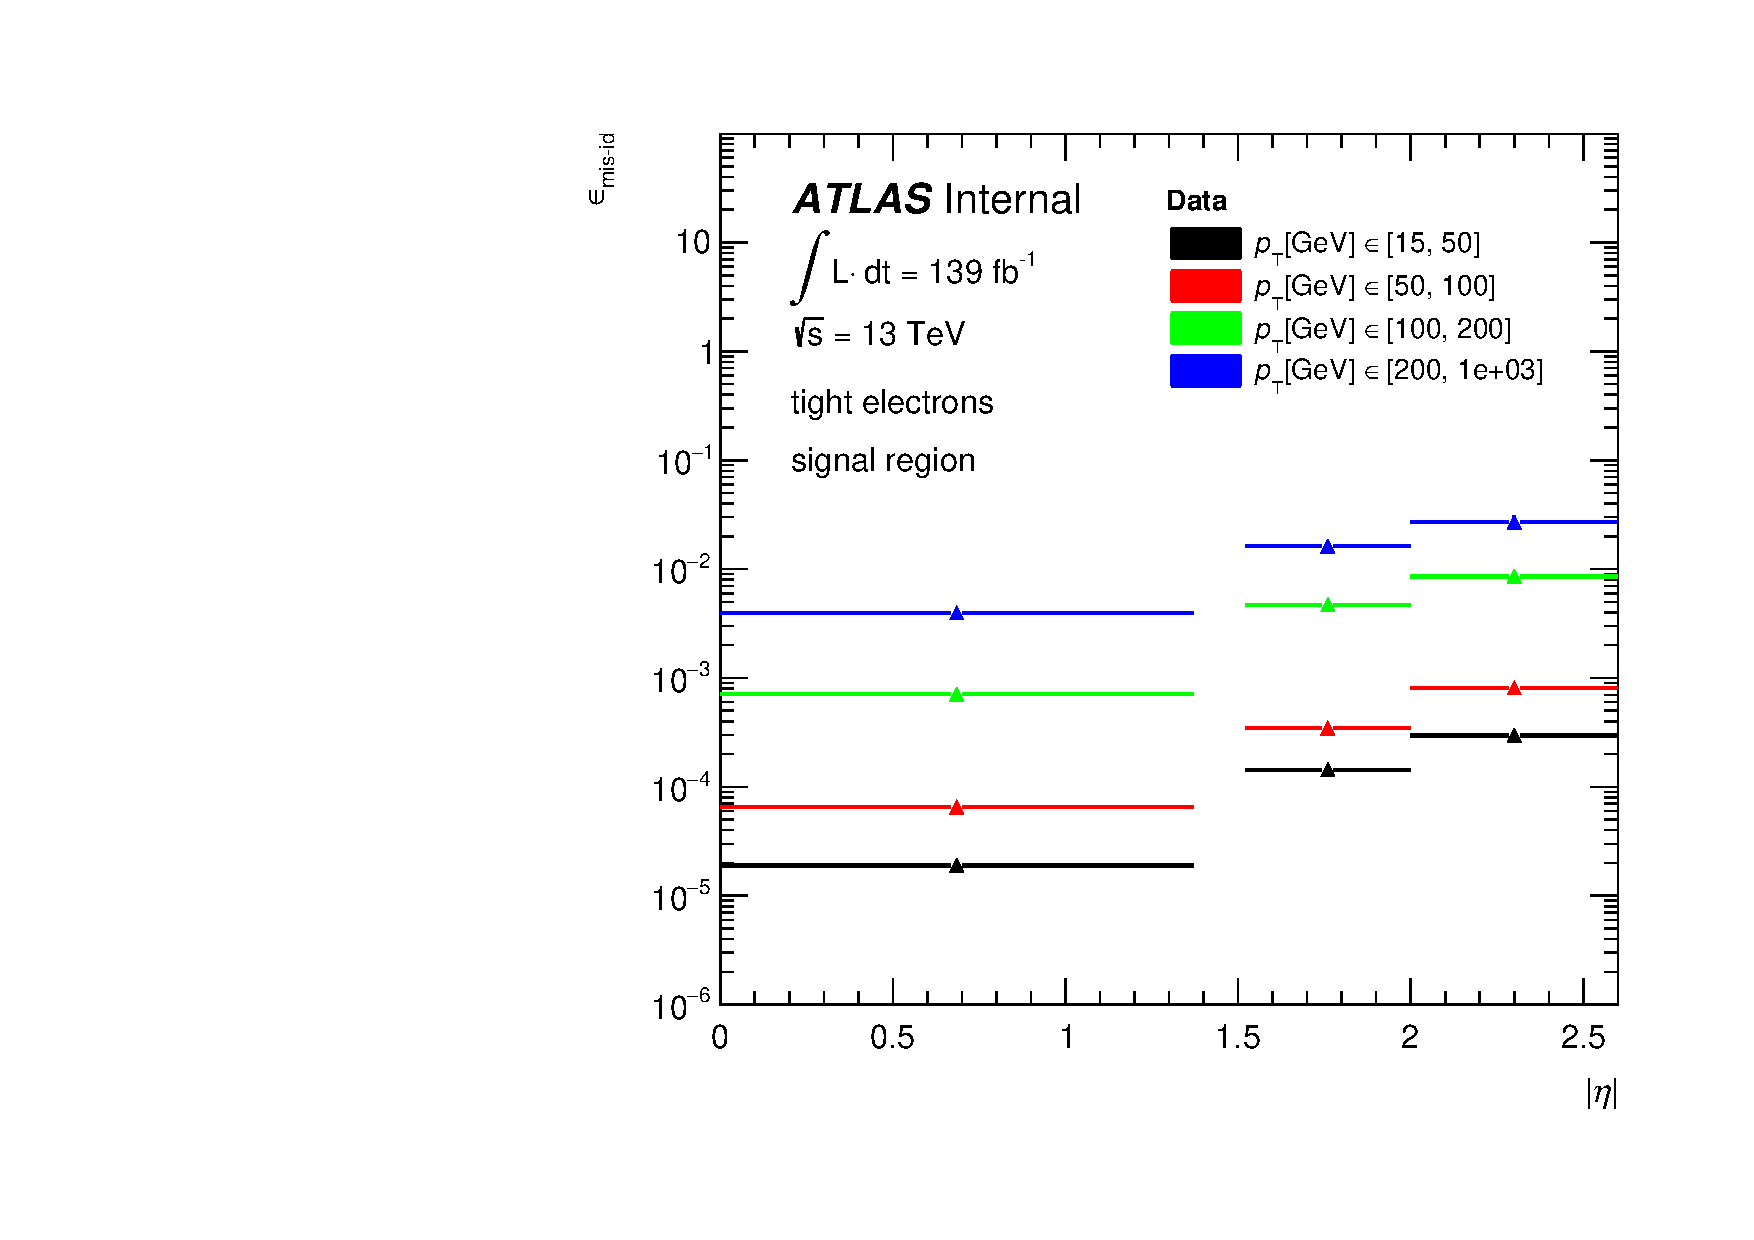
\includegraphics[width=0.37\textwidth]{figures/qmisid/crateData_tight_m2}}
  \caption{QMisID rates derived from the data with the likelihood method for tight electrons. 
           The rates are presented as a function of $|\eta|$ and parameterised in $\pT$ for the 
           photon-conversion CRs and the signal region. Due to lack of statistics, the
           the bins in $\pT$ are merged for the internal-conversion CR.\label{fig:Lik2Ddata}}
\end{figure}

%~~~~~~~~~~~~~~~~~~~~~~~~~~~~~~~~~~~~~~~~~~~~~~~~~~~~~~~~~~~~~~~
\subsubsection{Validation of the likelihood method (truth-closure)}
%~~~~~~~~~~~~~~~~~~~~~~~~~~~~~~~~~~~~~~~~~~~~~~~~~~~~~~~~~~~~~~~

To validate the likelihood method the QMisID rates are derived from simulated $Z$+jets events and compared to the 
rates based on the MC truth information (truth-matching). The comparison is shown in figure\,\ref{fig:LikTruthT} 
as a function of $|\eta|$ and parameterised in $\pT$. To mitigate the large statistical uncertainties introduced due 
to the size of the MC sample, the $|\eta|$-bins are merged. Furthermore, for the internal conversion region, $\pT$ 
bins are also merged. The results show no significant disagreement between the two approaches. Any difference is 
considered as a systematic uncertainty to the rates (see section\,\ref{Sec:systematic}). Finally, the same comparison 
is presented for the case of anti-tight electrons in order to verity the agreement of the two approaches with 
higher statistics.  

\begin{figure}[tb!]
  \centering
  {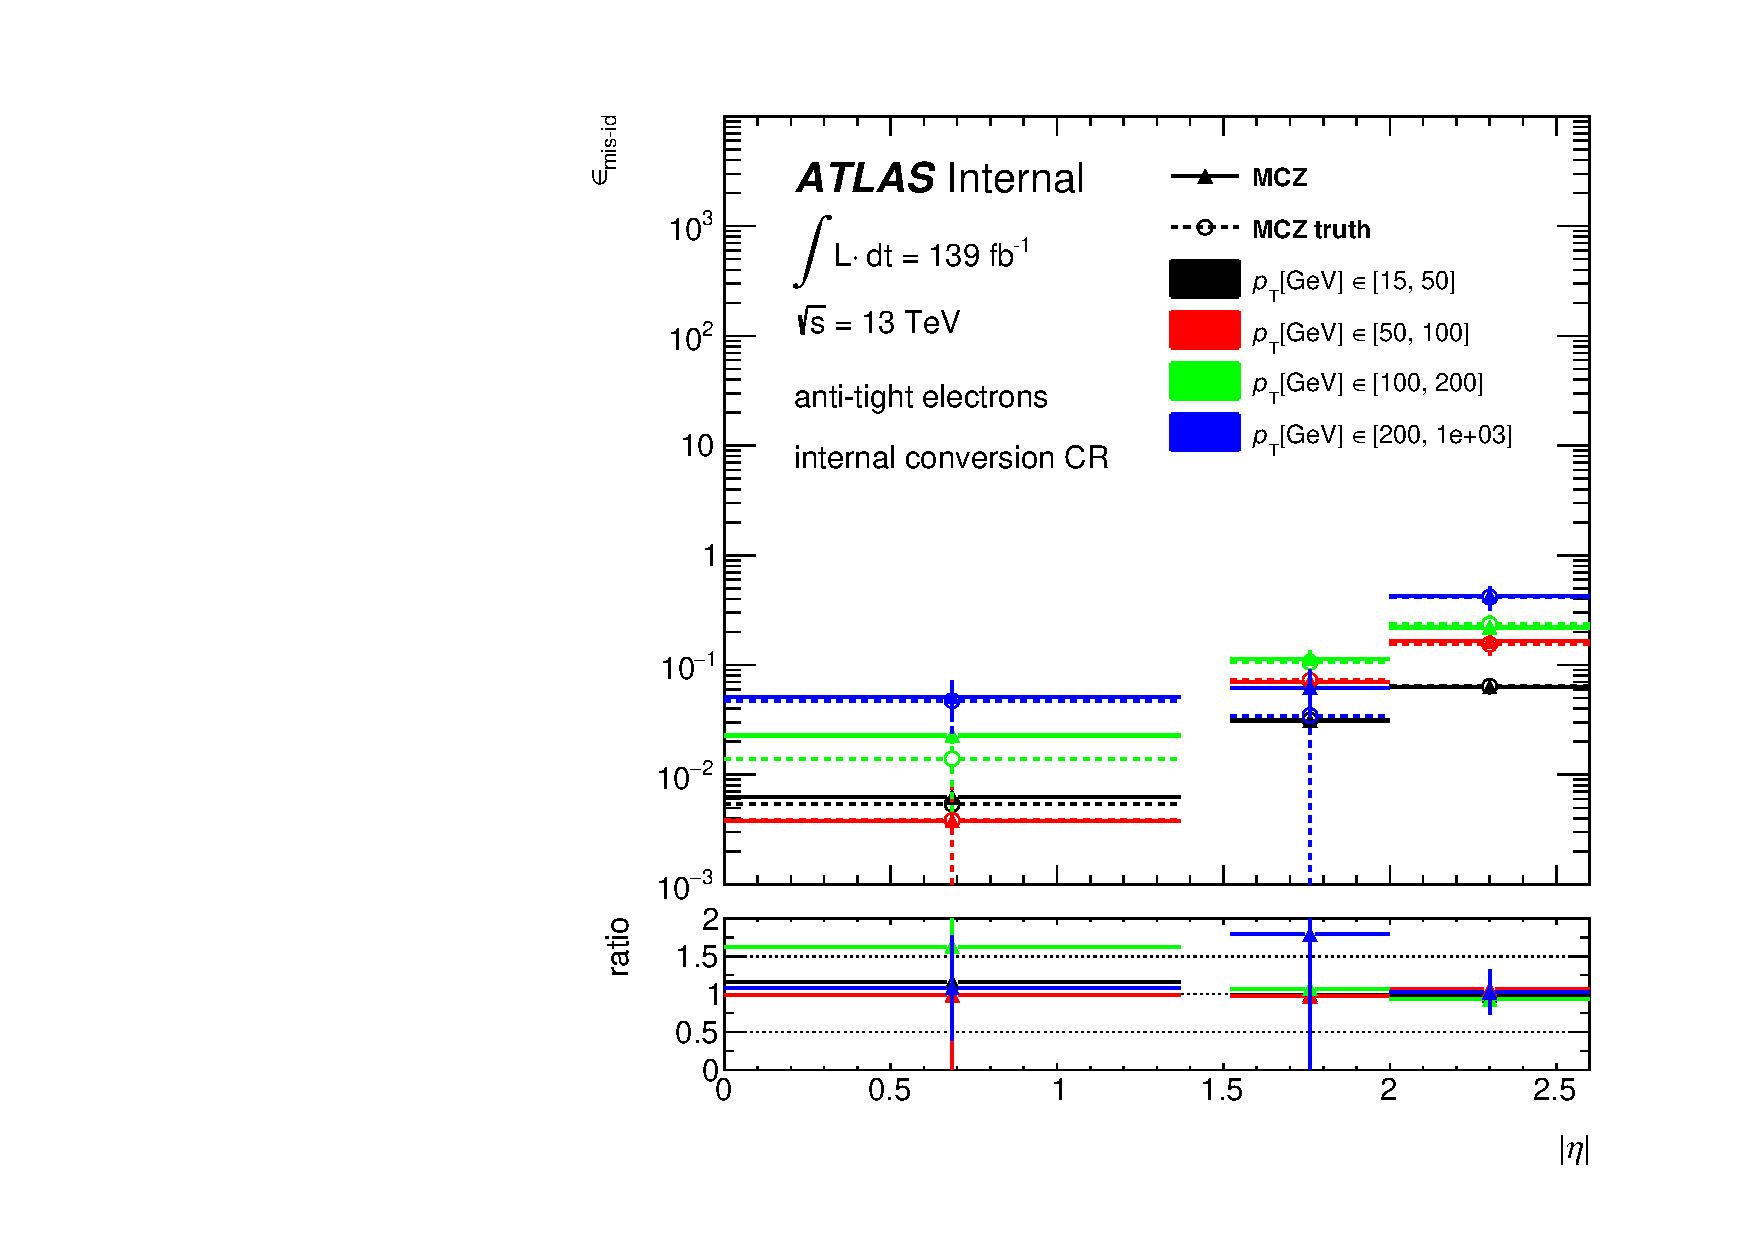
\includegraphics[width=0.45\textwidth]{figures/qmisid/crateMCZ_MCZtruth_atight_m0}}
  {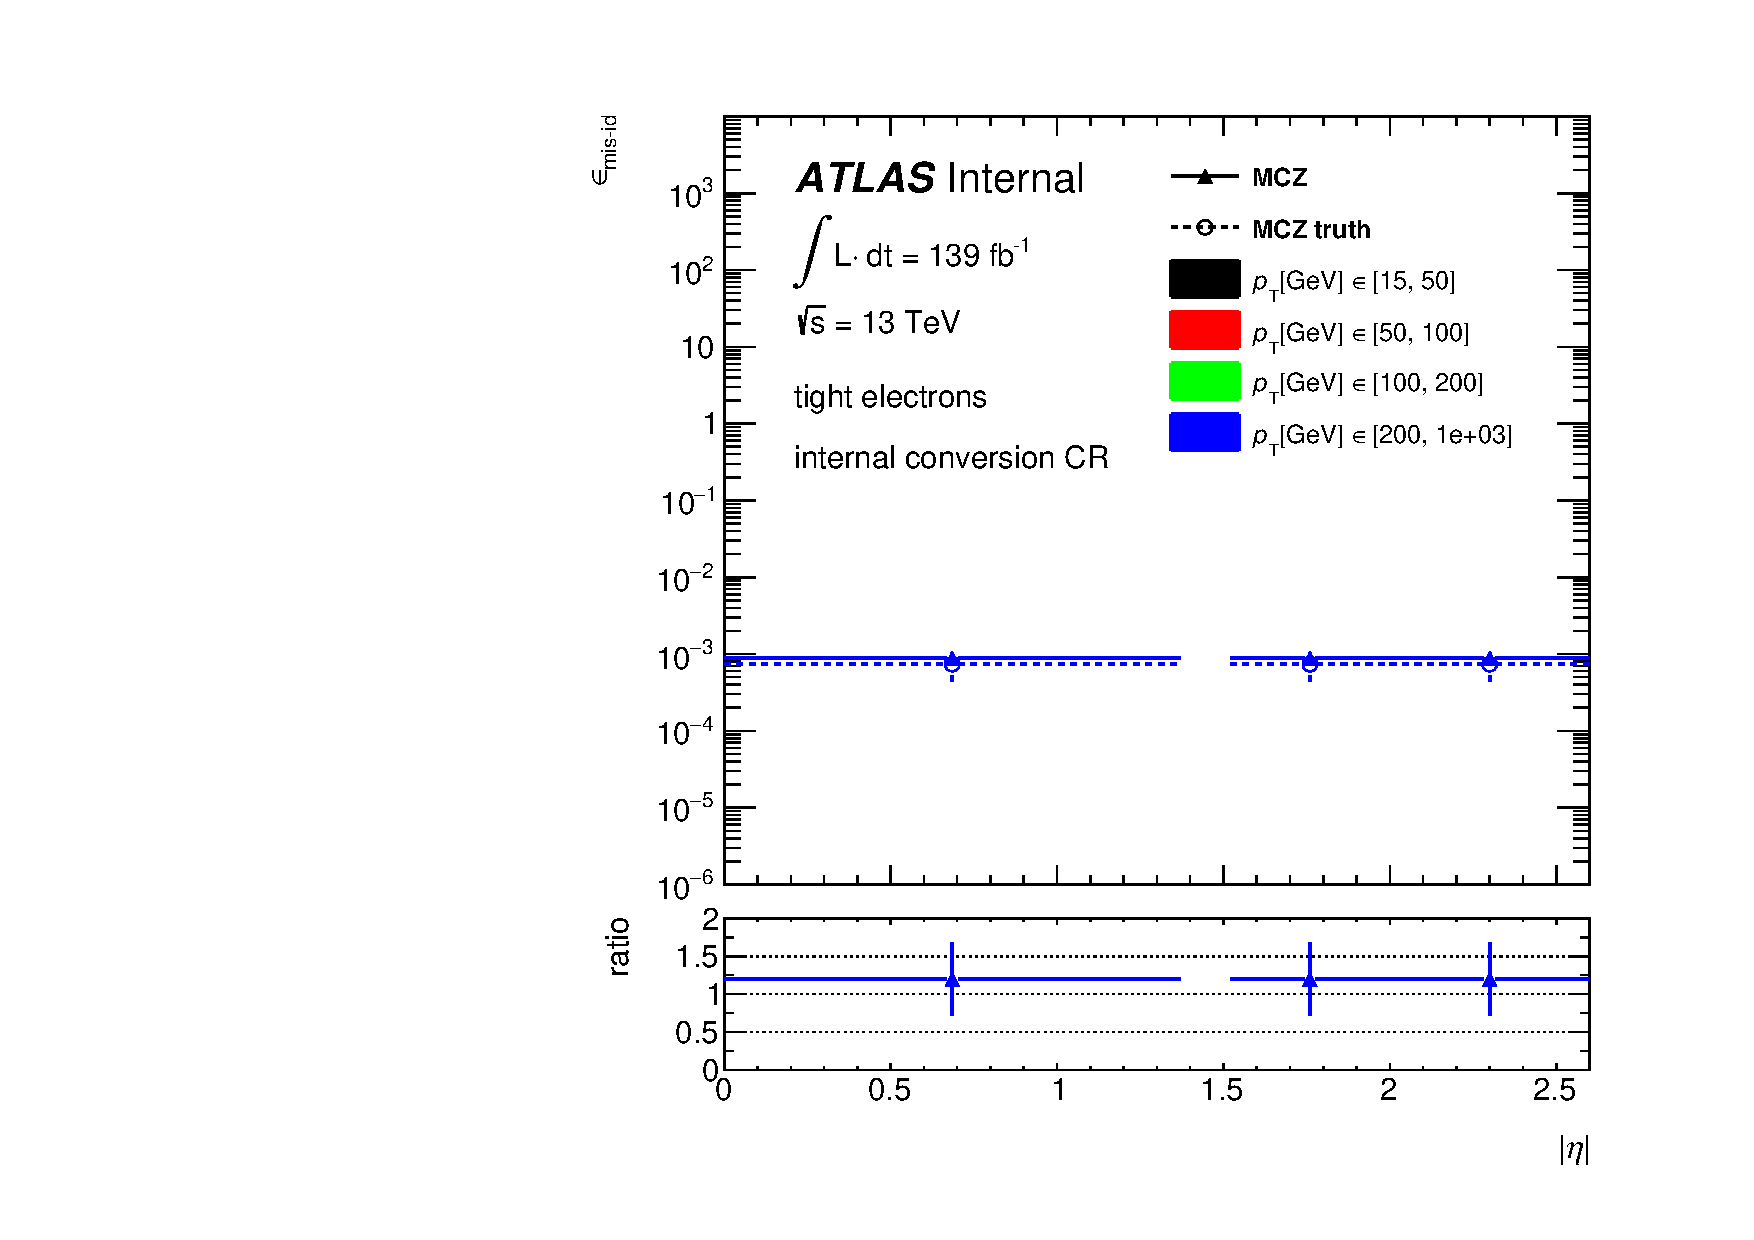
\includegraphics[width=0.45\textwidth]{figures/qmisid/crateMCZ_MCZtruth_tight_m0}}\\
  {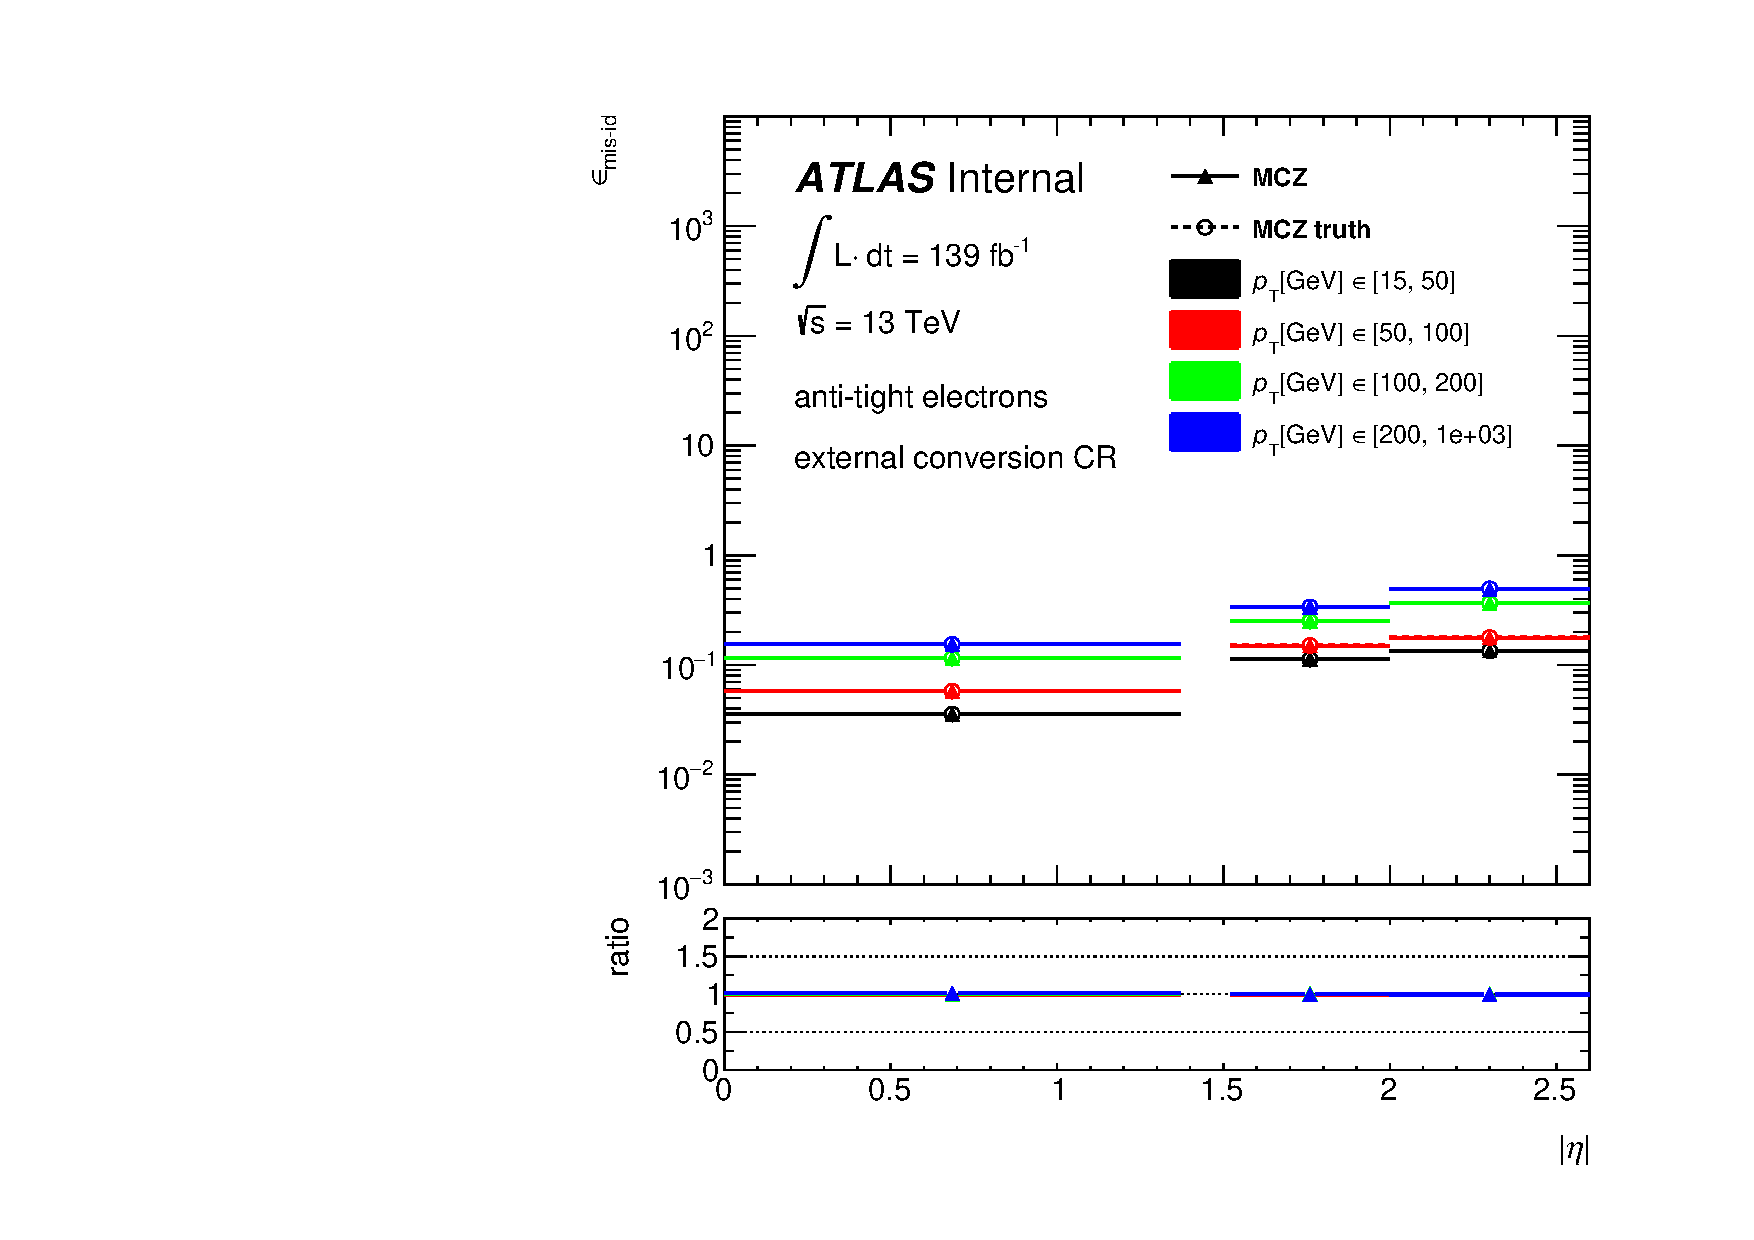
\includegraphics[width=0.45\textwidth]{figures/qmisid/crateMCZ_MCZtruth_atight_m1}}
  {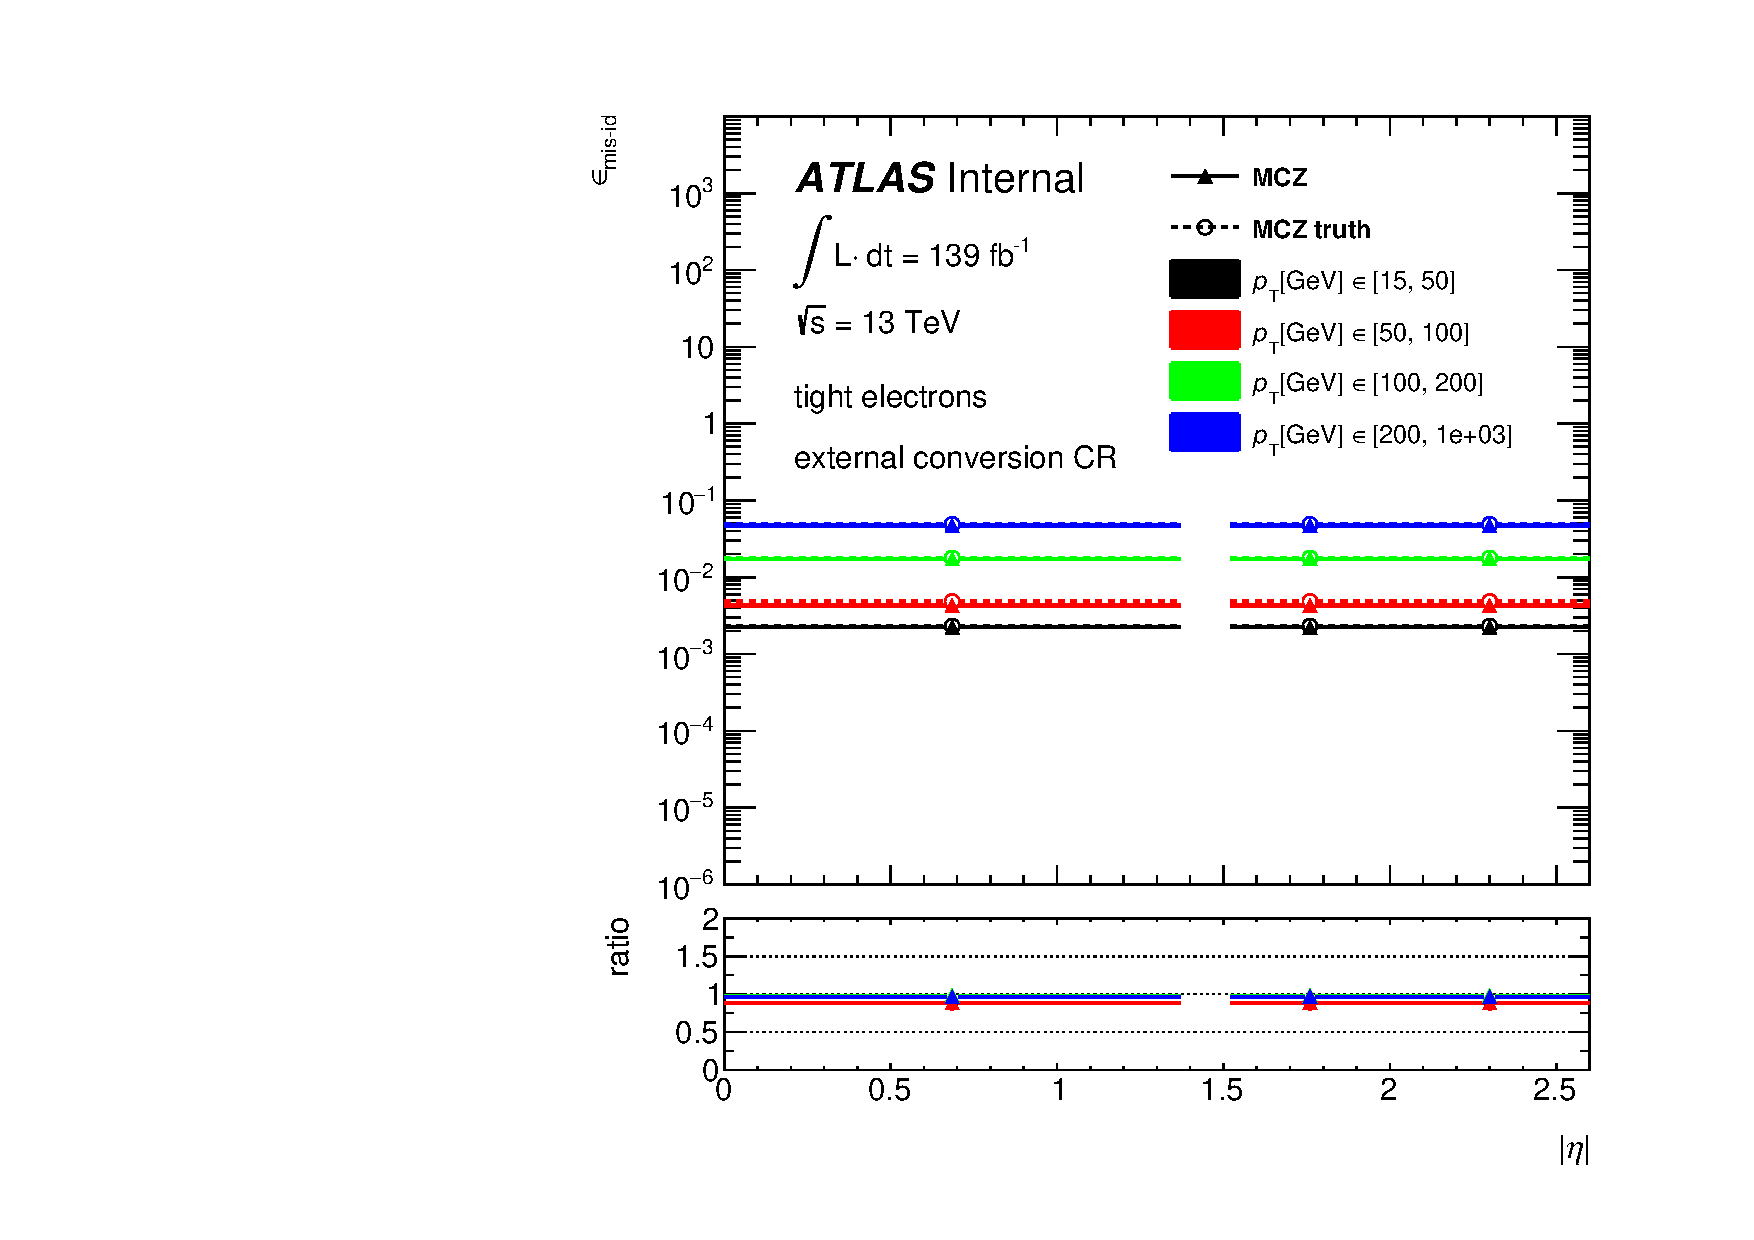
\includegraphics[width=0.45\textwidth]{figures/qmisid/crateMCZ_MCZtruth_tight_m1}}\\
  {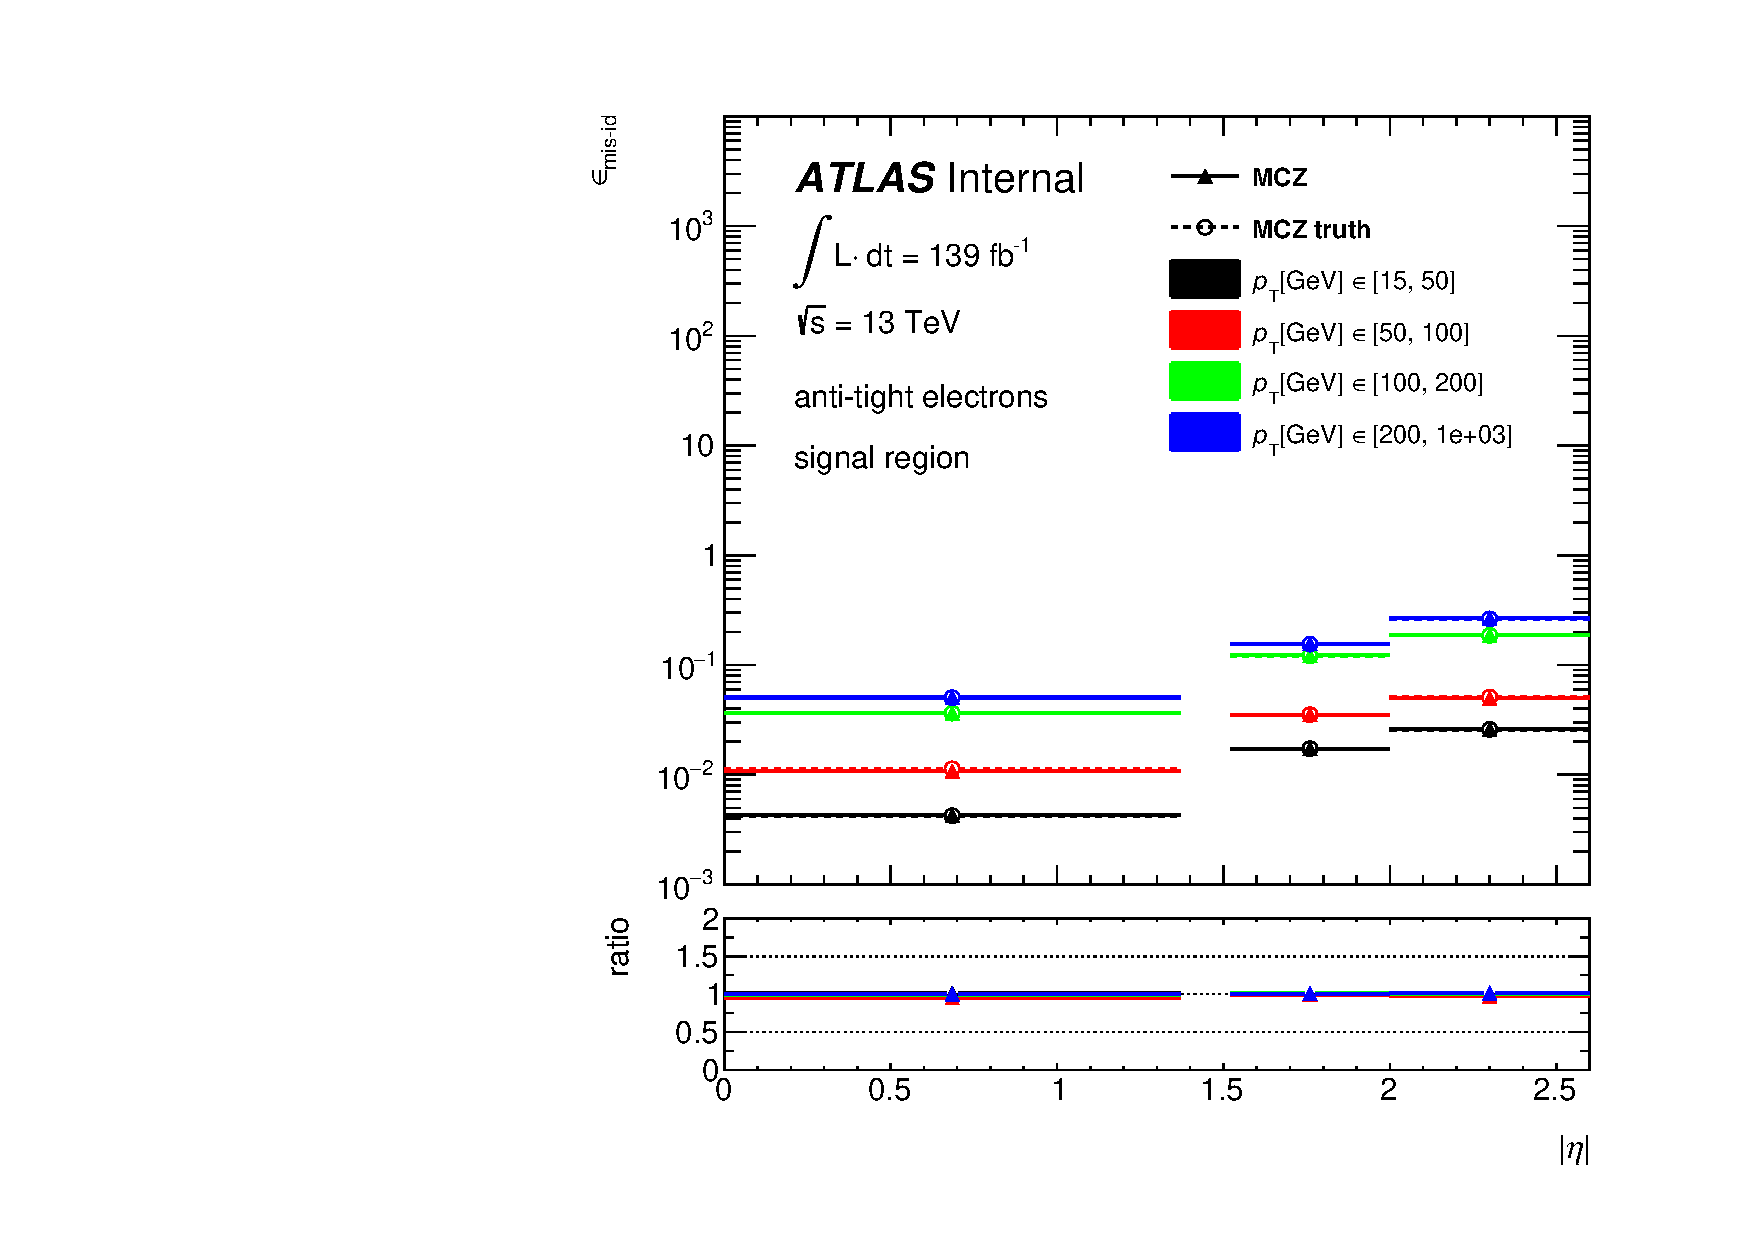
\includegraphics[width=0.45\textwidth]{figures/qmisid/crateMCZ_MCZtruth_atight_m2}}
  {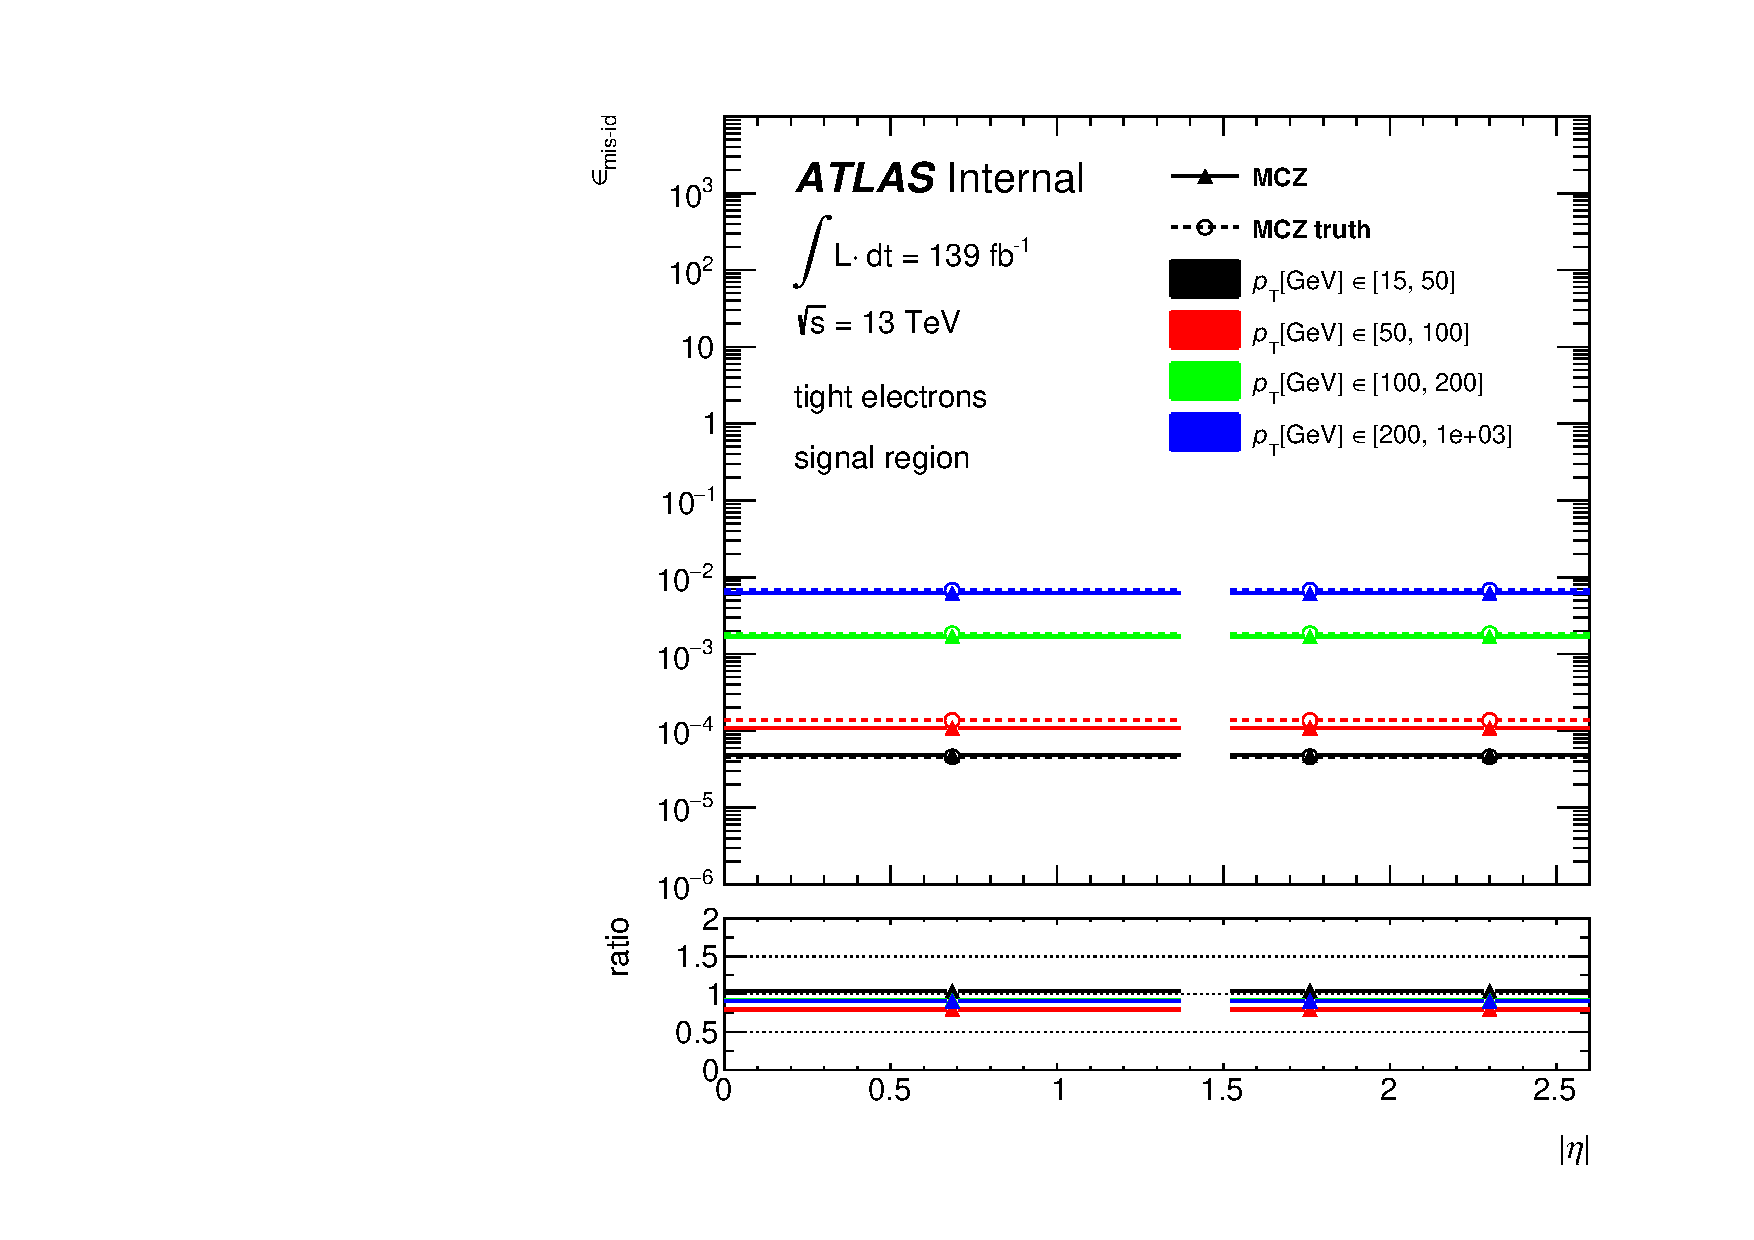
\includegraphics[width=0.45\textwidth]{figures/qmisid/crateMCZ_MCZtruth_tight_m2}}
  \caption{QMisID rates derived from $Z\rightarrow ee$ simulated events with the likelihood method, compared to truth-based
           rates for anti-tight (left) and tight (right) electrons. The rates are presented as a function of $|\eta|$,
           parameterised in $\pT$ for the photon-conversion CRs and the signal region. Due to lack of statistics, in 
           the case of tight electrons, the bins in $|\eta|$ are merged. For the internal-conversion CR, the bins in 
           $\pT$ are also merged.\label{fig:LikTruthT}}
\end{figure}

\clearpage

%~~~~~~~~~~~~~~~~~~~~~~~~~~~~~~~~~~~
\subsubsection{Systematic uncertainties}
\label{Sec:systematic}
%~~~~~~~~~~~~~~~~~~~~~~~~~~~~~~~~~~~

Four sources of systematic uncertainties are assigned to the QMisiD rates:

\begin{itemize}
\item the error estimates from the likelihood maximisation (figure\,\ref{fig:QMisID:systa}) which depend on the 
      statistical size of the control region of the data in which the rates are estimated;
\item the difference between the rates measured with the likelihood method and those obtained by truth-matching 
      with simulated $Z\rightarrow ee$ events (figure\,\ref{fig:QMisID:systa});
\item the variation of the rates with the $m_Z$ window
  (figure\,\ref{fig:QMisID:systb});
\item low $m_{ee}$ mismodelings observed on simulated $t\bar{t}$ samples and
  that can be relevant to some control regions.
\end{itemize}

The total uncertainty is defined as the quadratic sum of the above contributions (figure\,\ref{fig:QMisID:systb}).

\begin{figure}[p!]
  \begin{center}
  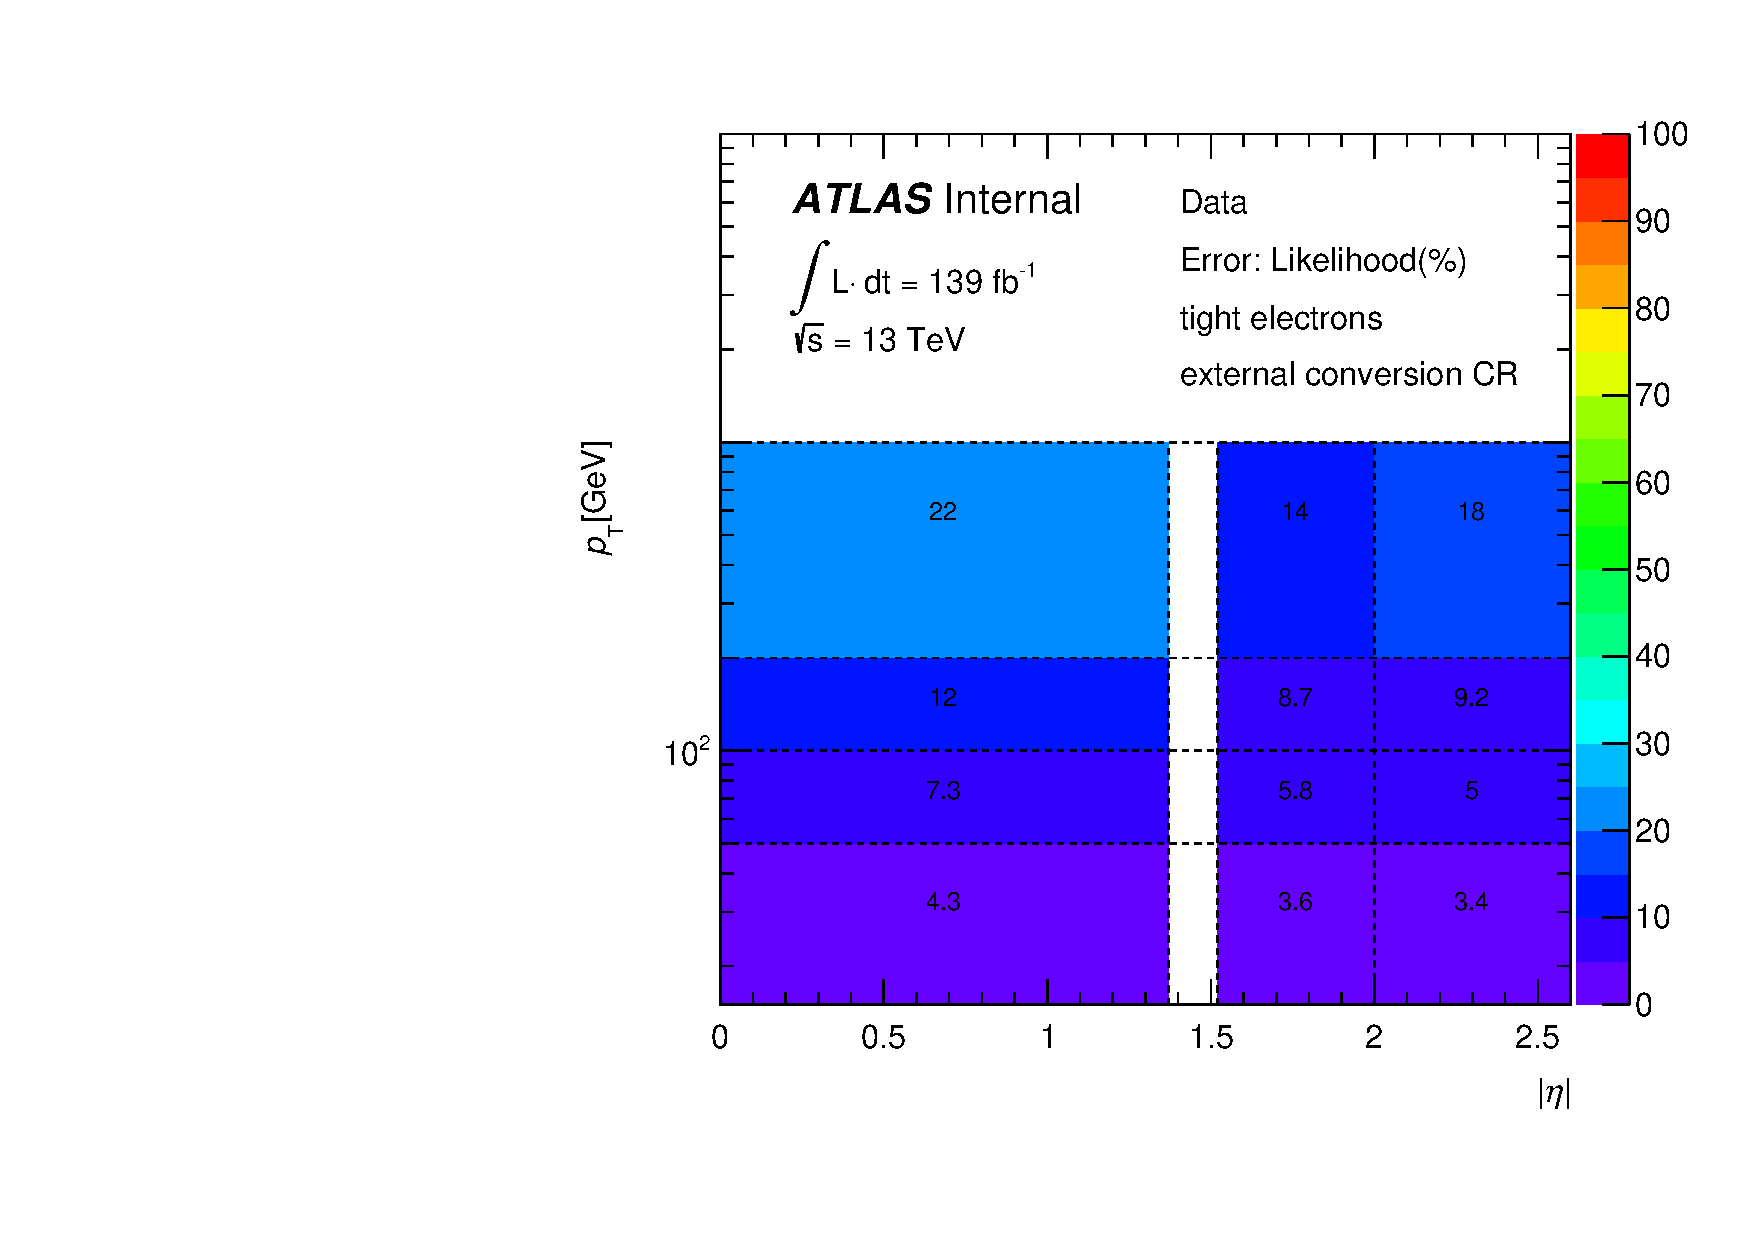
\includegraphics[width=0.45\textwidth]{figures/qmisid/syst_Data_Likelihood_tight_extcr}
  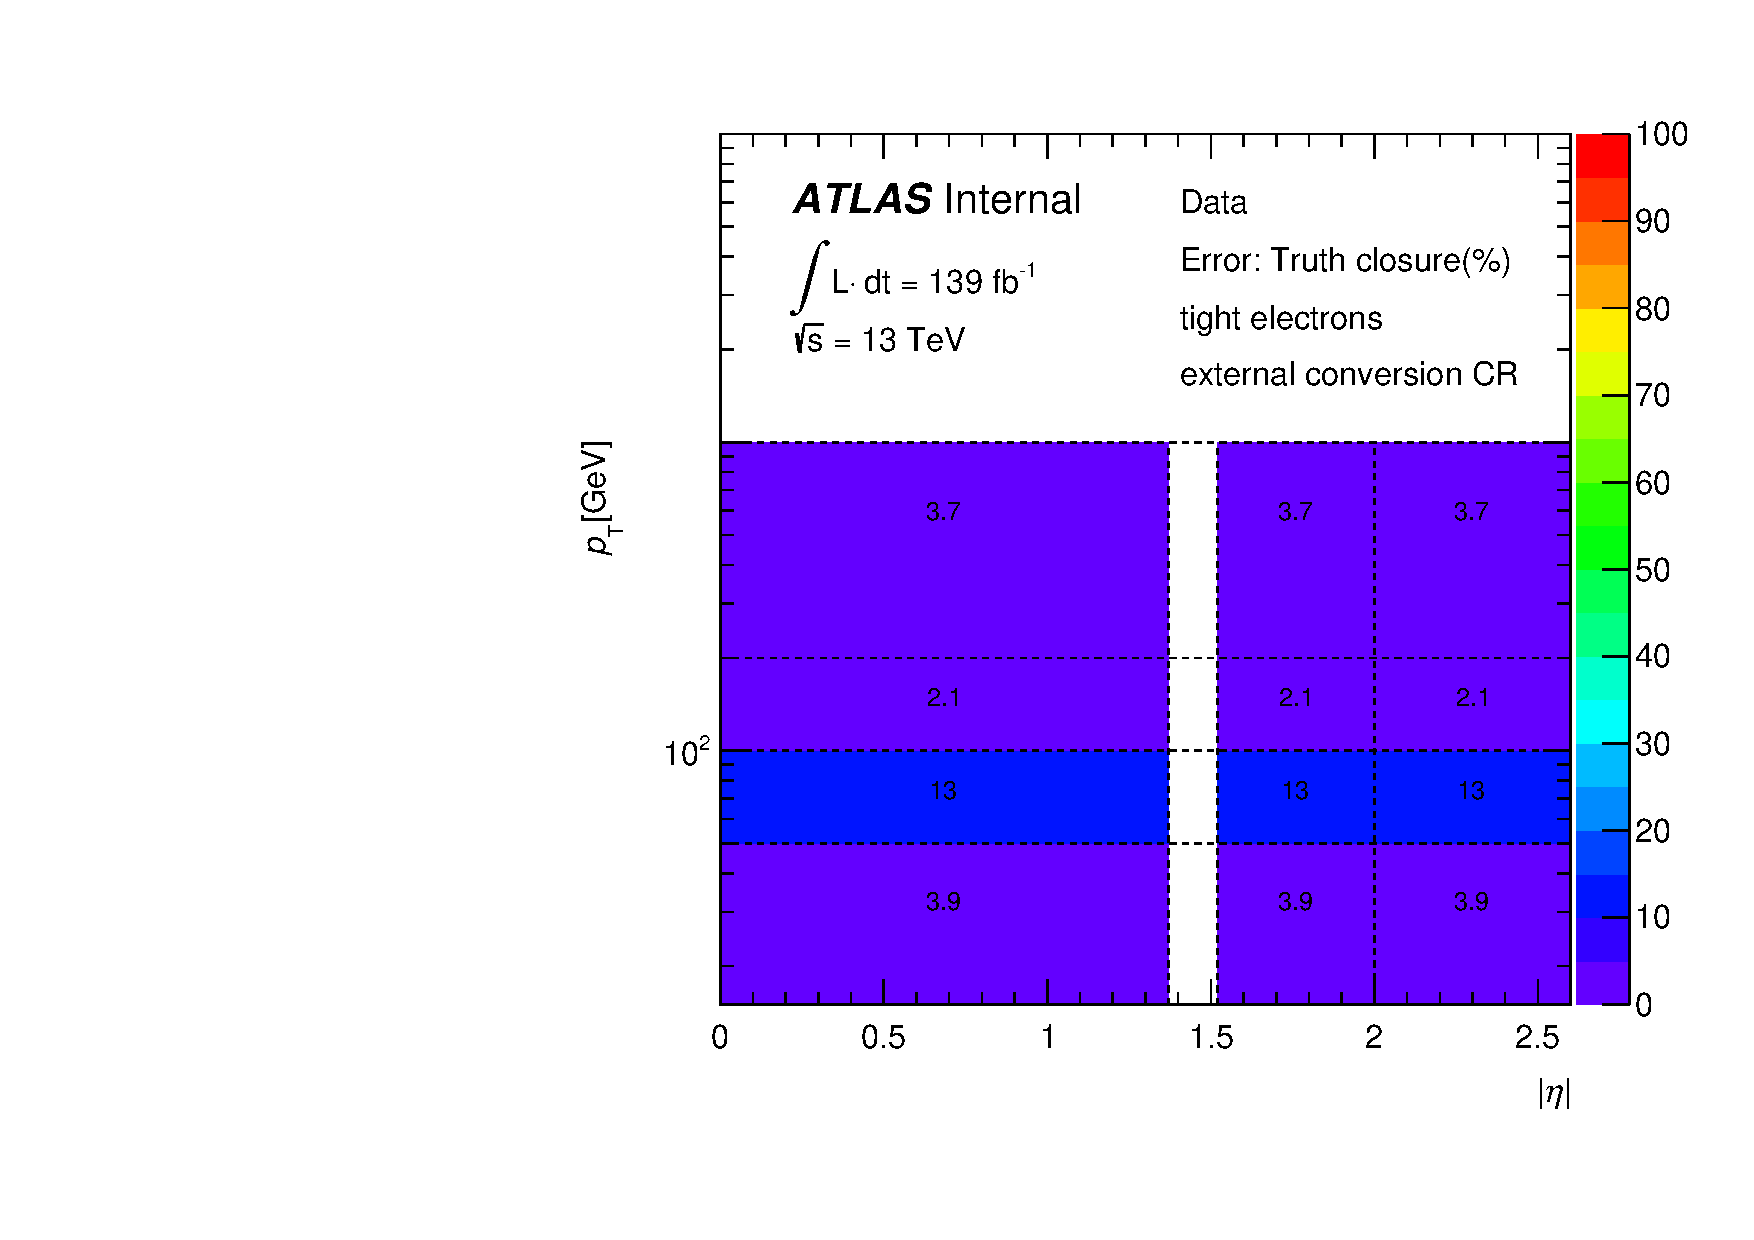
\includegraphics[width=0.45\textwidth]{figures/qmisid/syst_Data_Truthclosure_tight_extcr}\\
  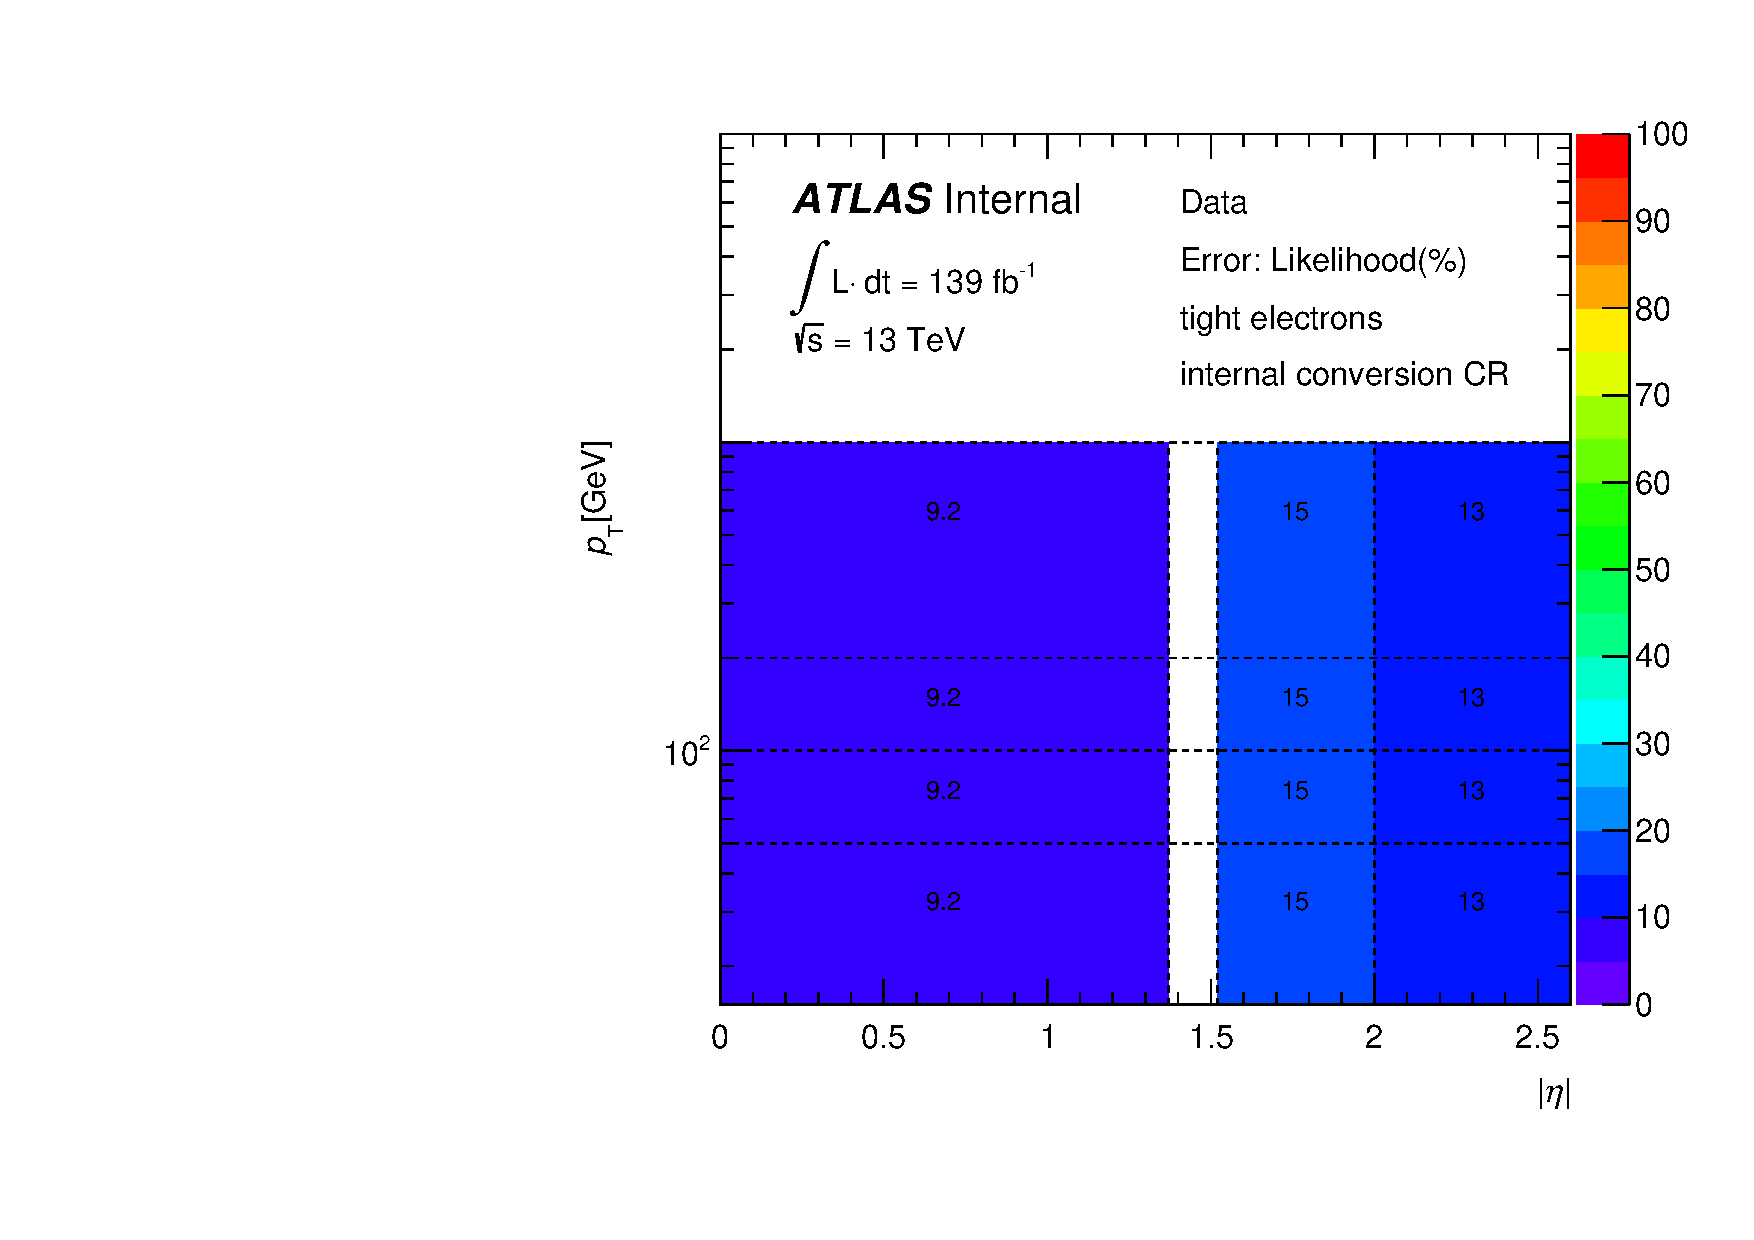
\includegraphics[width=0.45\textwidth]{figures/qmisid/syst_Data_Likelihood_tight_intcr}
  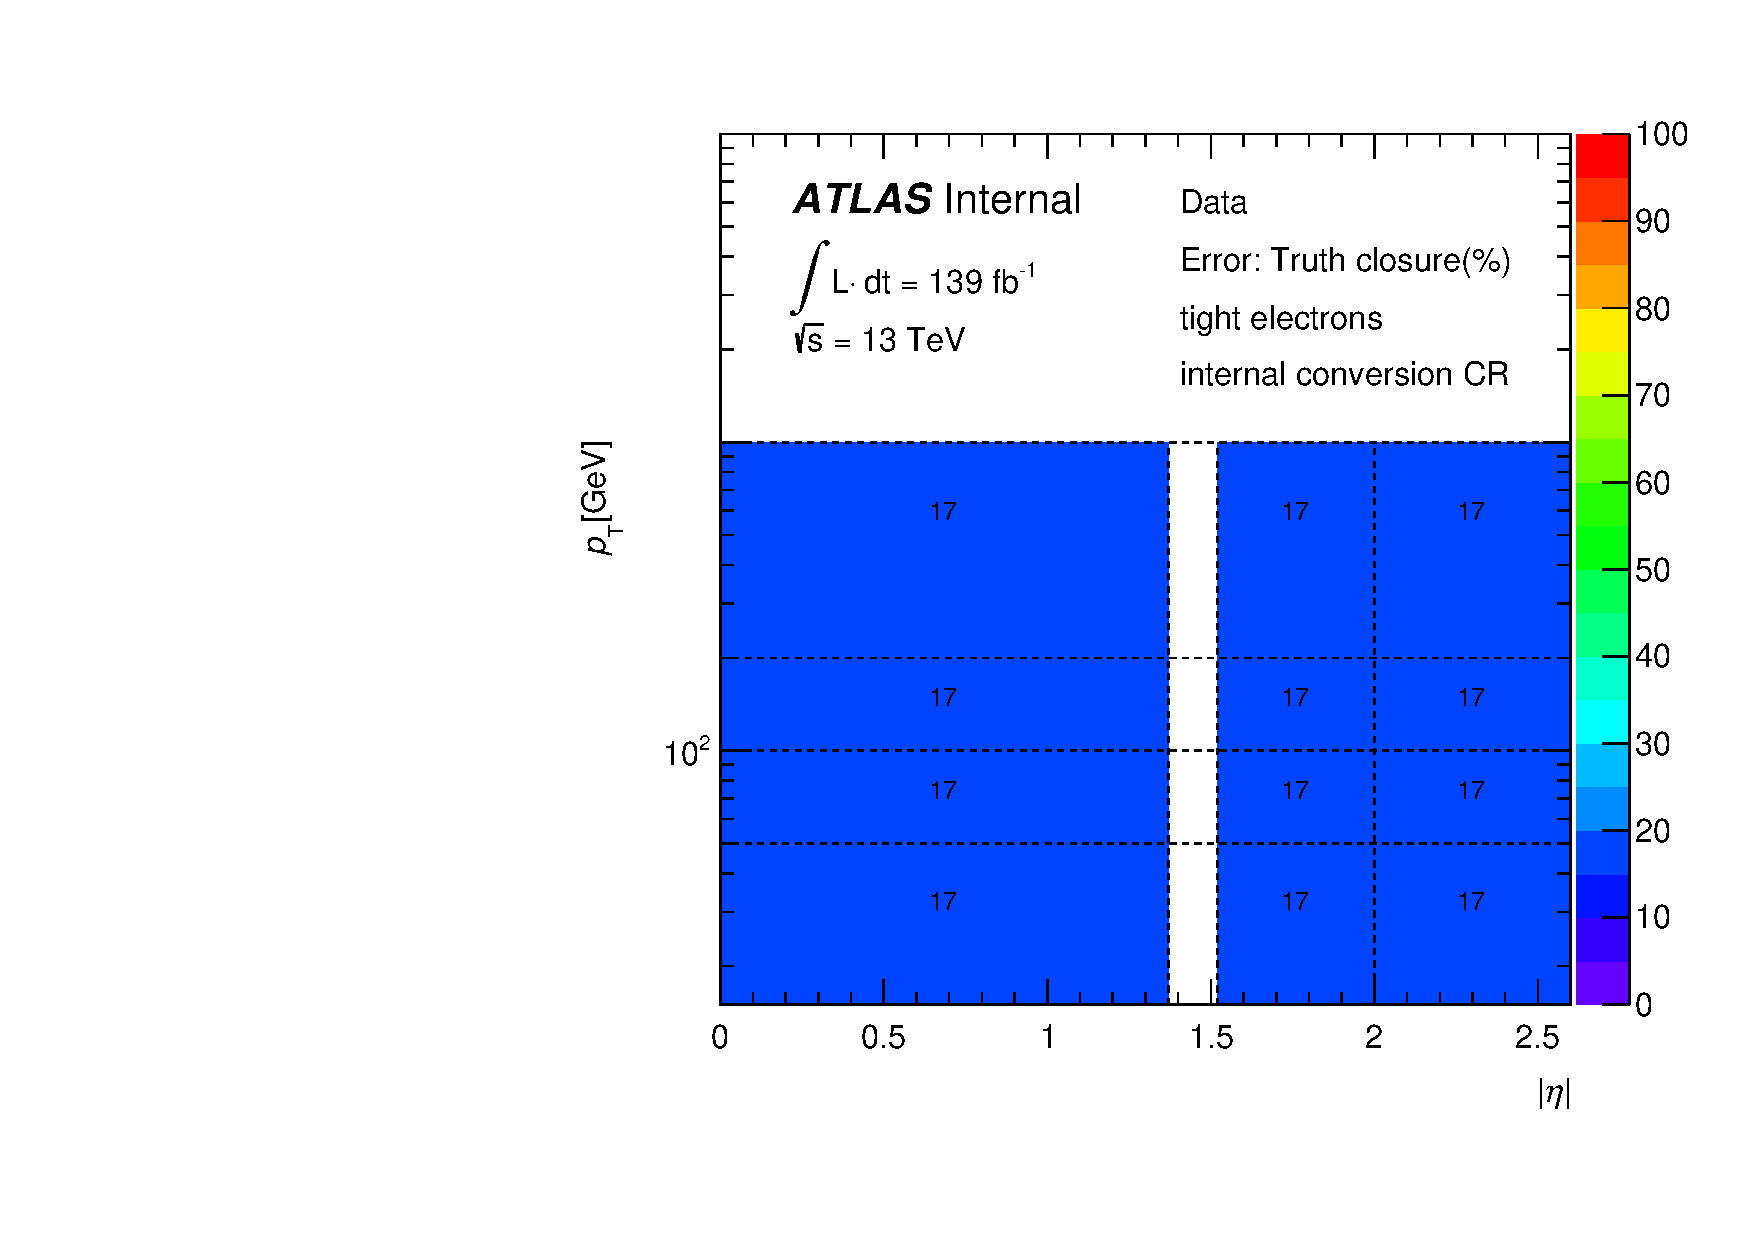
\includegraphics[width=0.45\textwidth]{figures/qmisid/syst_Data_Truthclosure_tight_intcr}\\
  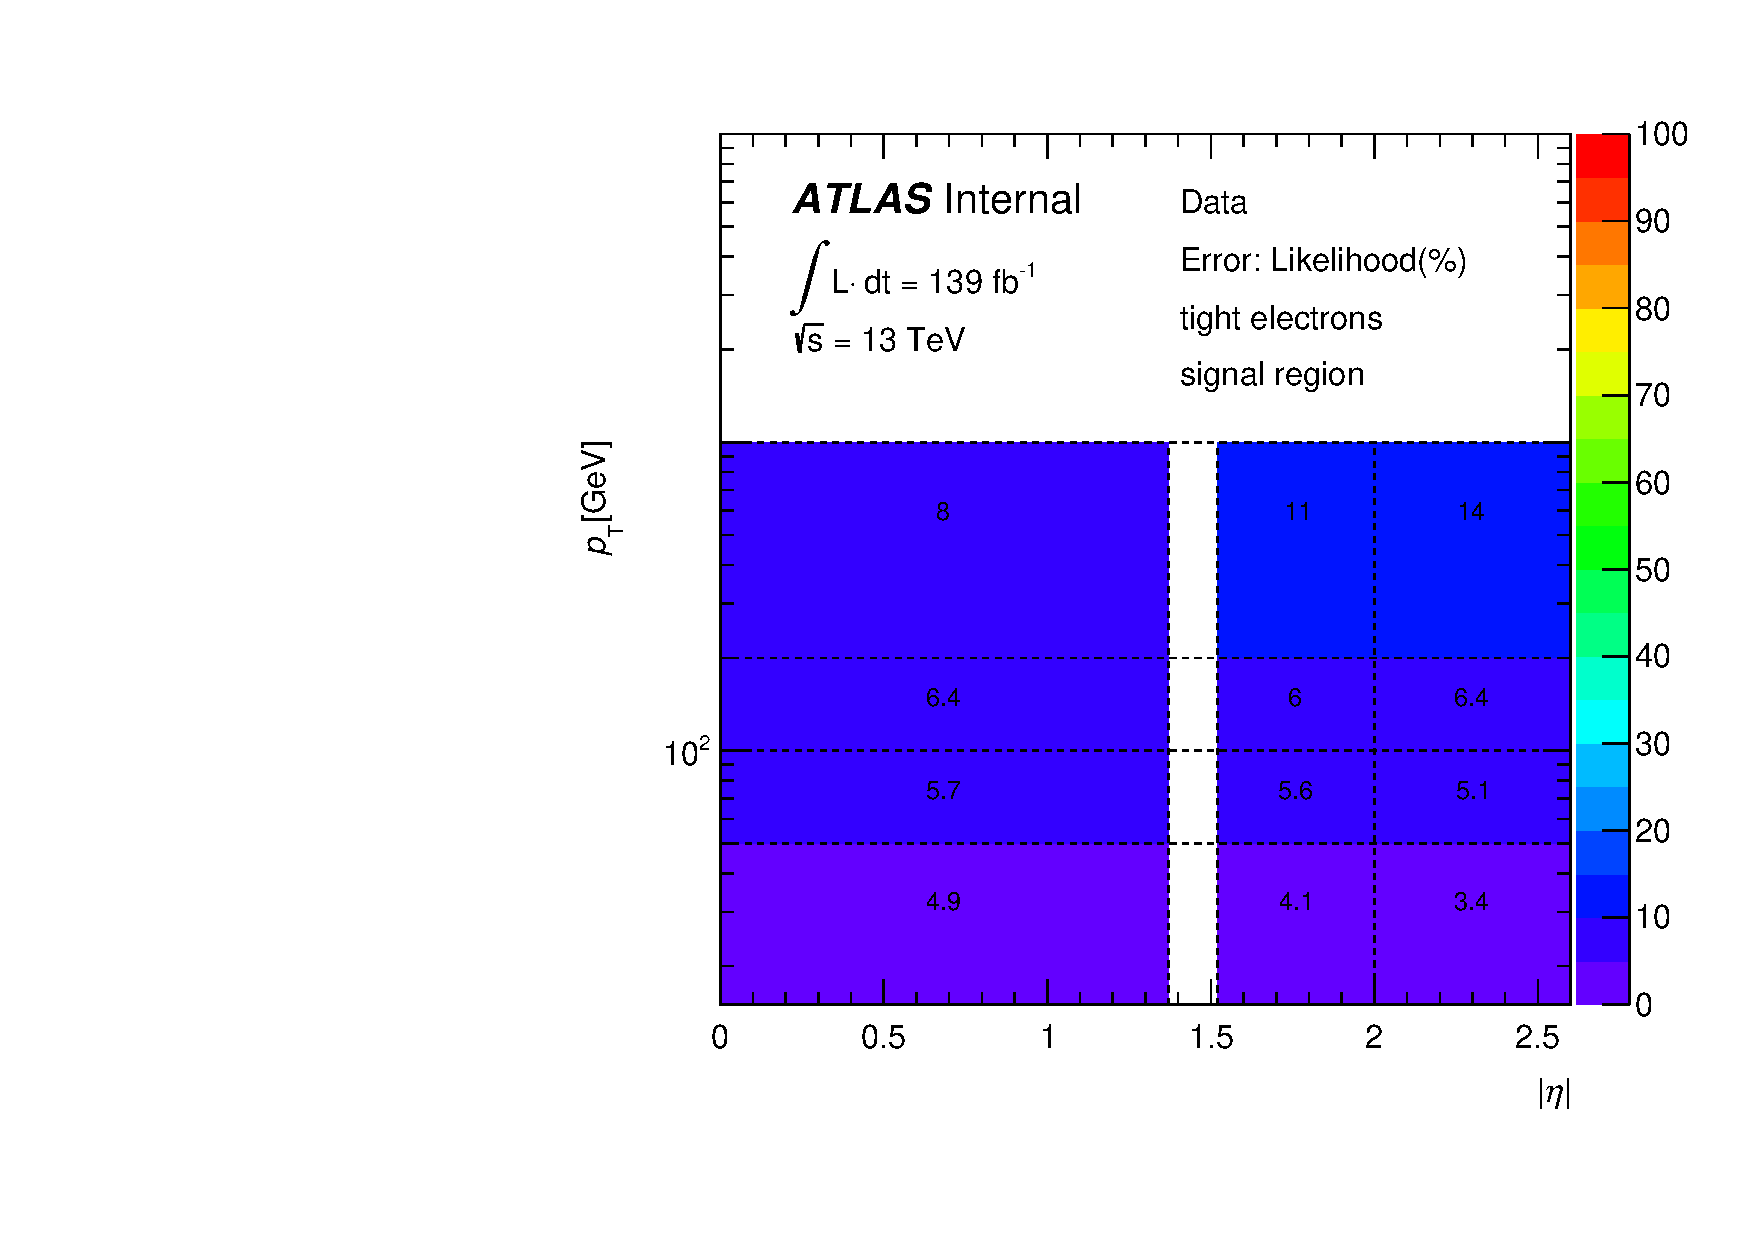
\includegraphics[width=0.45\textwidth]{figures/qmisid/syst_Data_Likelihood_tight_sr}
  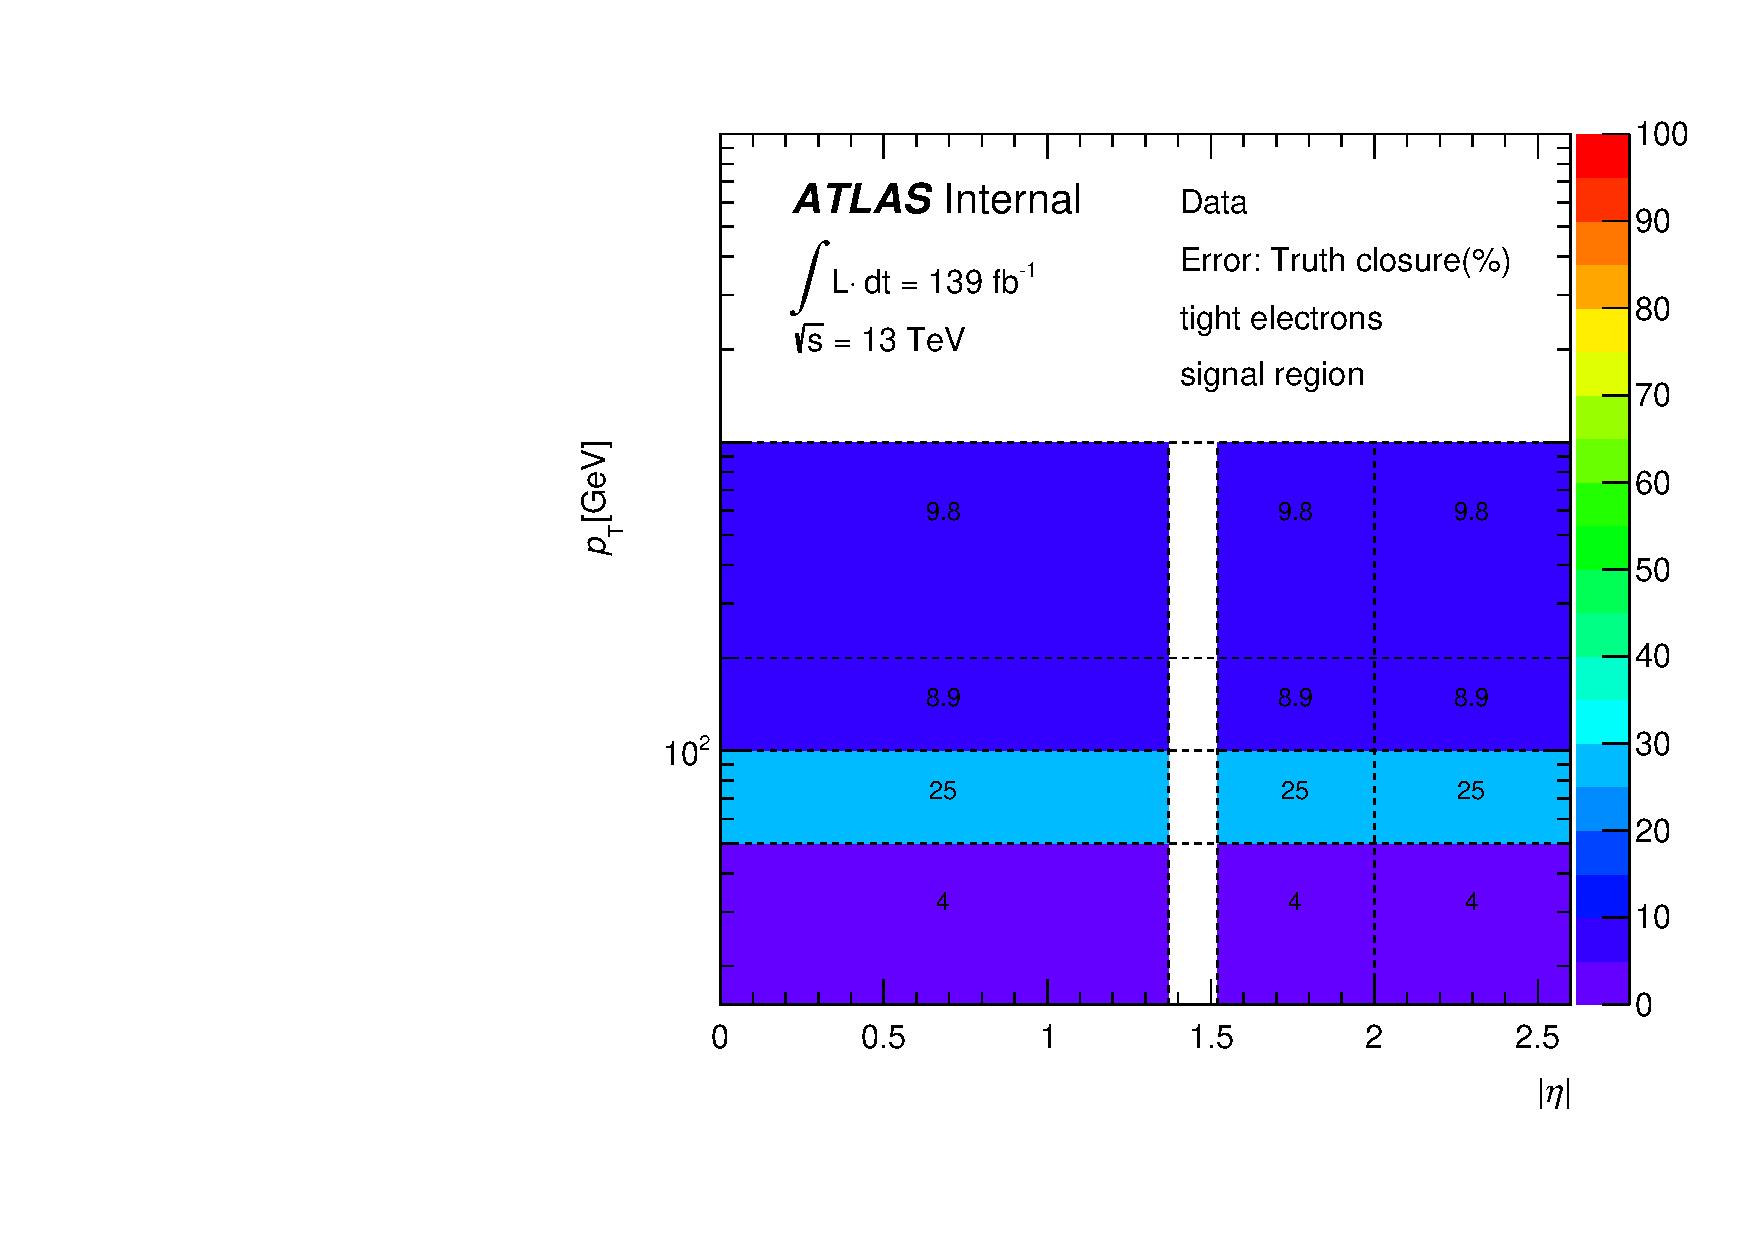
\includegraphics[width=0.45\textwidth]{figures/qmisid/syst_Data_Truthclosure_tight_sr}
  \caption{ \label{fig:QMisID:systa} Left: systematic uncertainty (\%), introduced from the statistical size of the control 
            region of the data that is used in the likelihood method, in bins of $|\eta|$ and $\pT$. Right: systematic uncertainty 
            (\%), introduced from the comparison of rates obtained from simulated $Z\rightarrow ee$ events with the likelihood 
            method to truth-based rates.}
  \end{center}
\end{figure}

\begin{figure}[p!]
  \begin{center}
  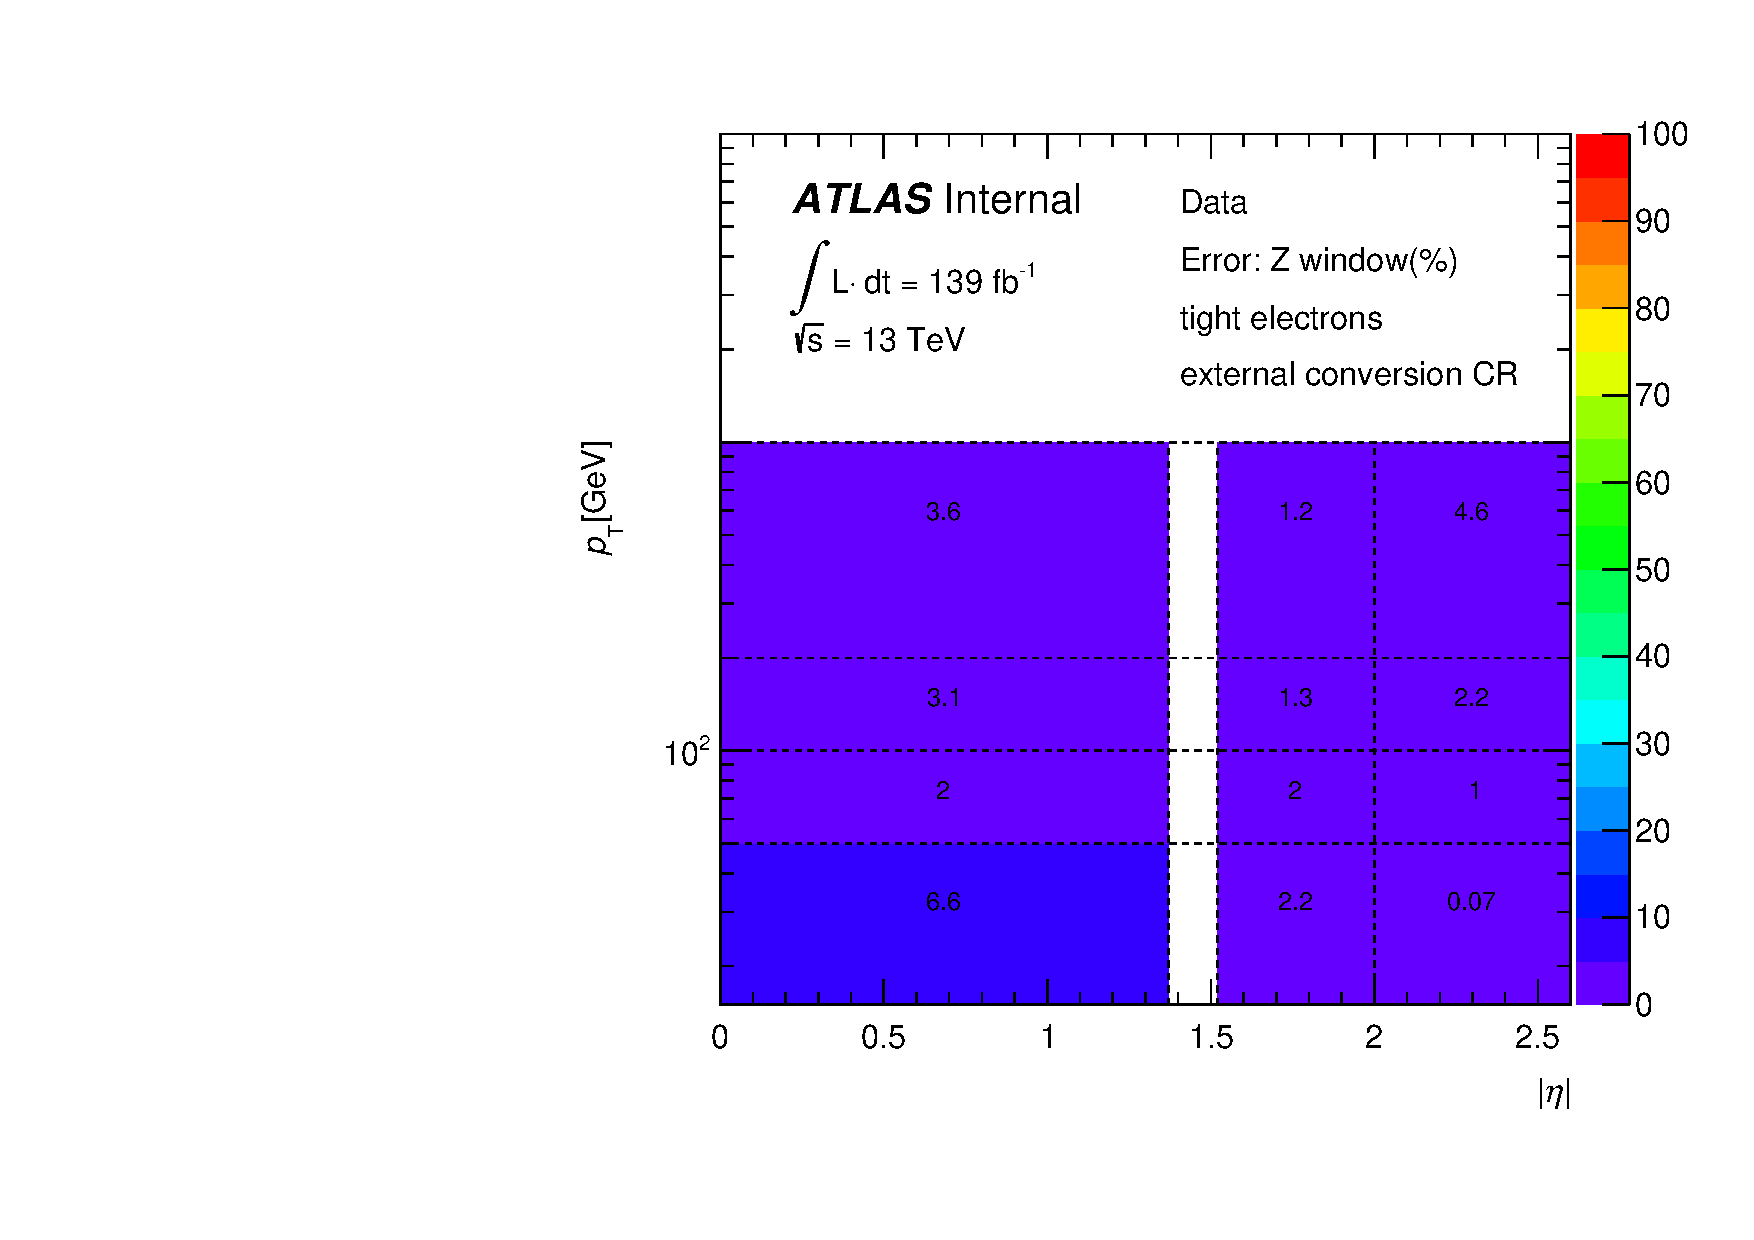
\includegraphics[width=0.45\textwidth]{figures/qmisid/syst_Data_Zwindow_tight_extcr}
  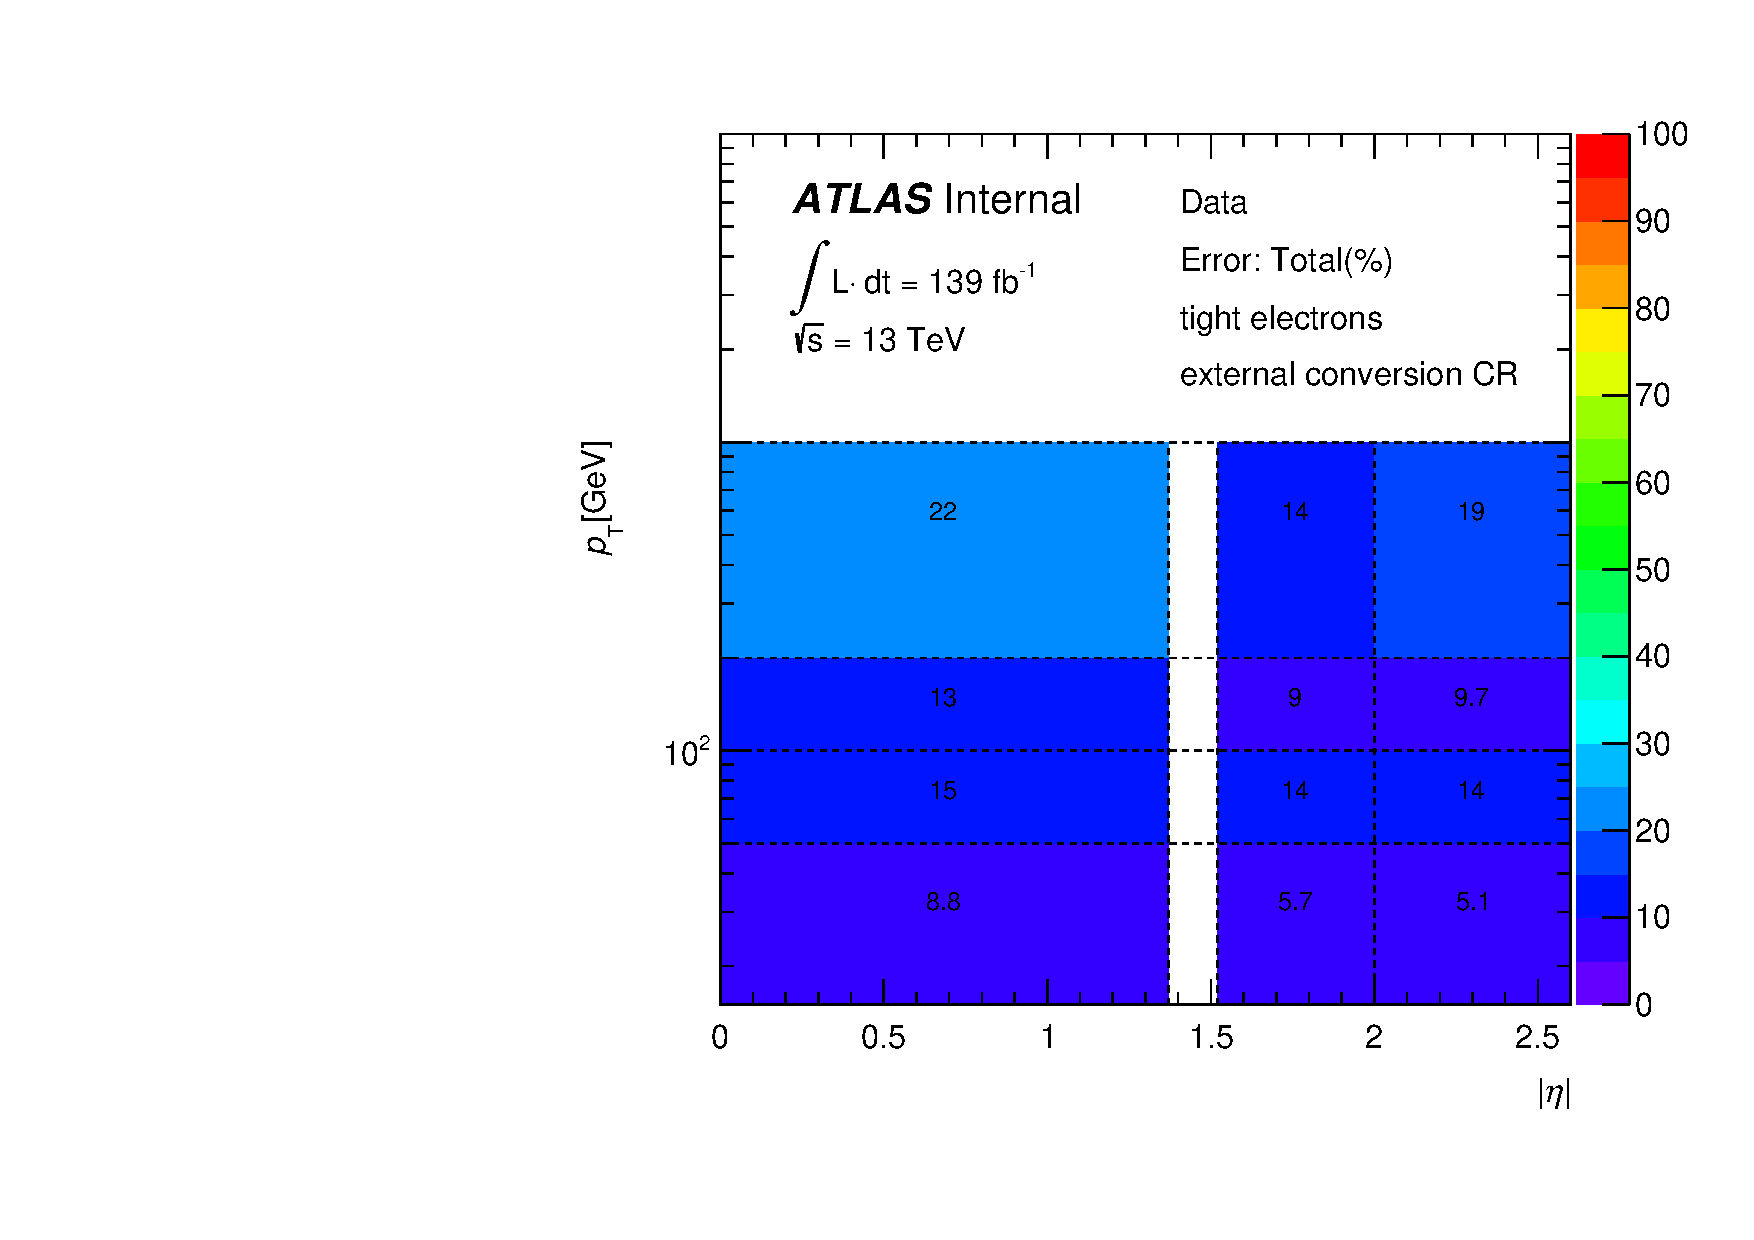
\includegraphics[width=0.45\textwidth]{figures/qmisid/syst_Data_Total_tight_extcr}\\
  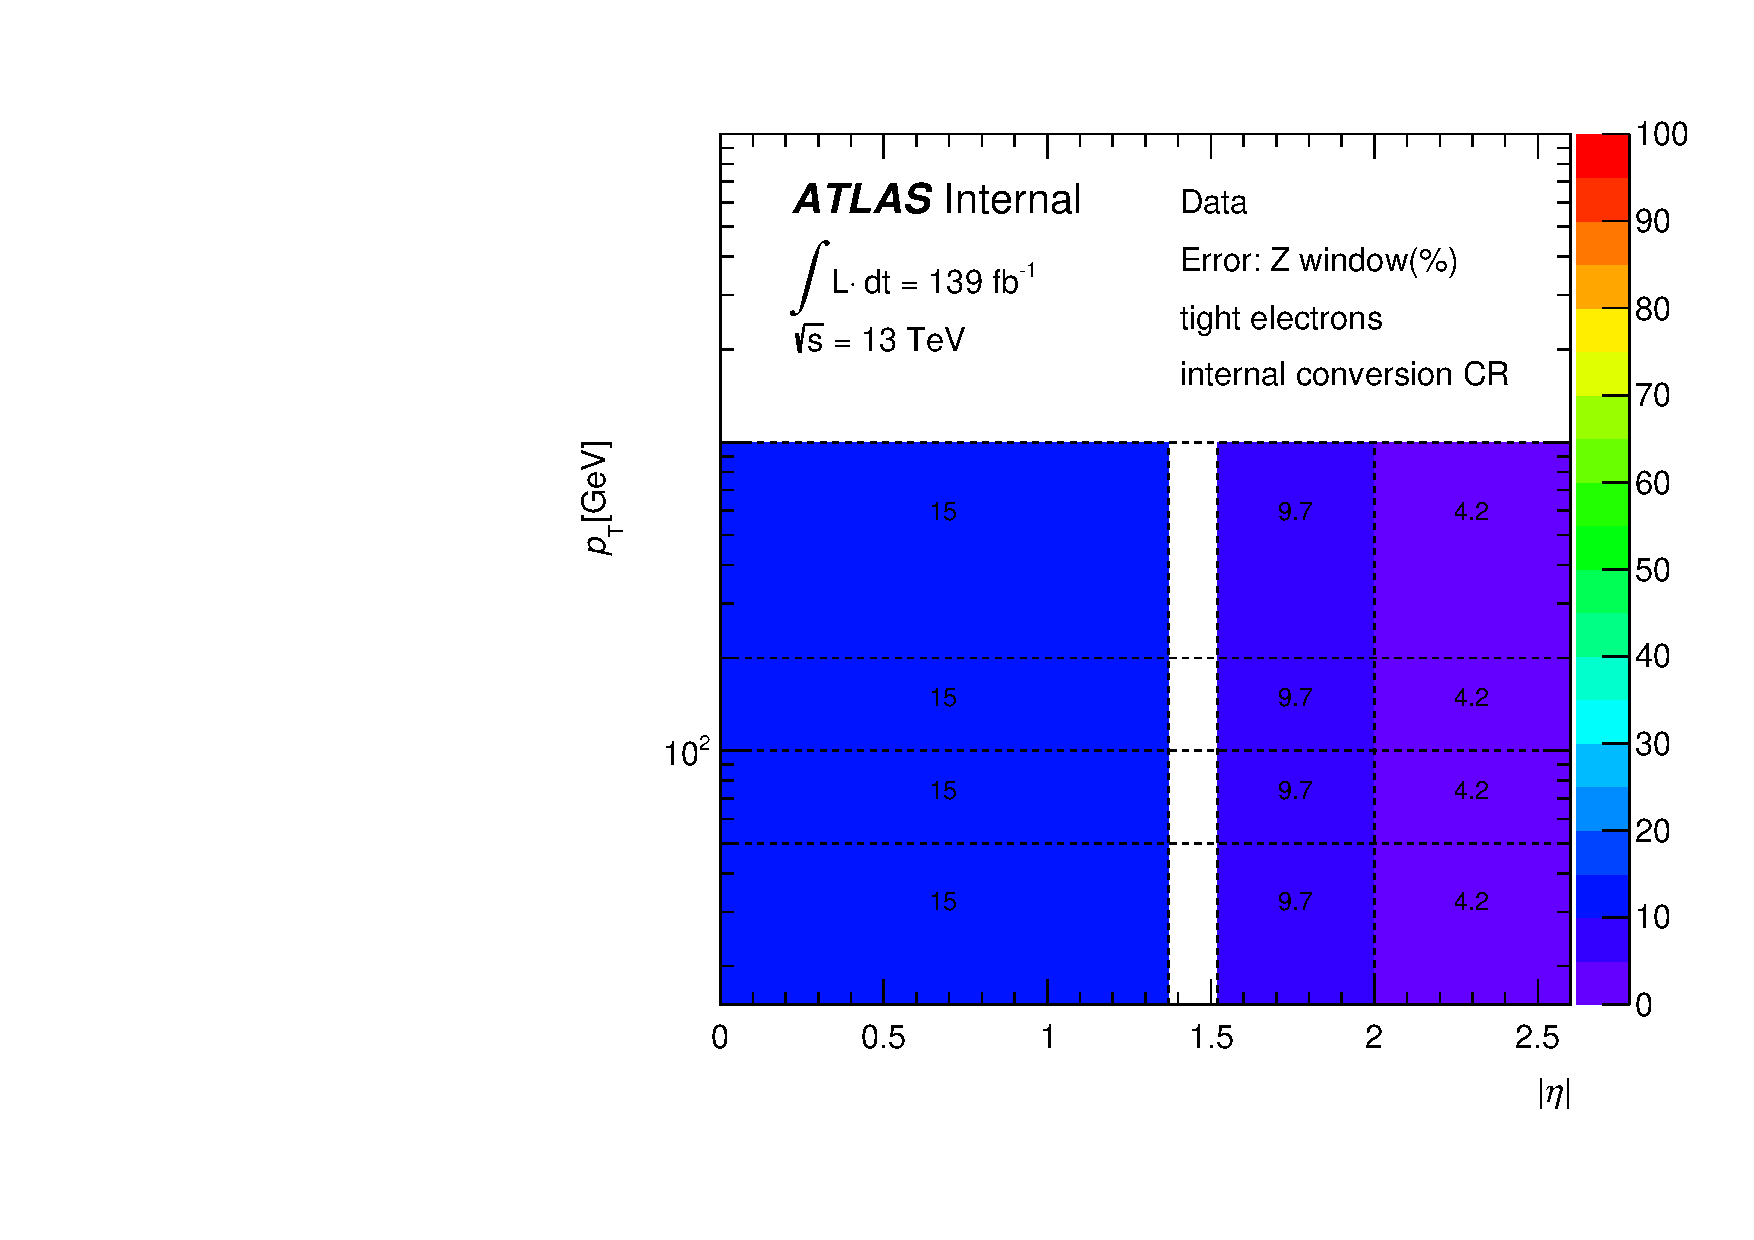
\includegraphics[width=0.45\textwidth]{figures/qmisid/syst_Data_Zwindow_tight_intcr}
  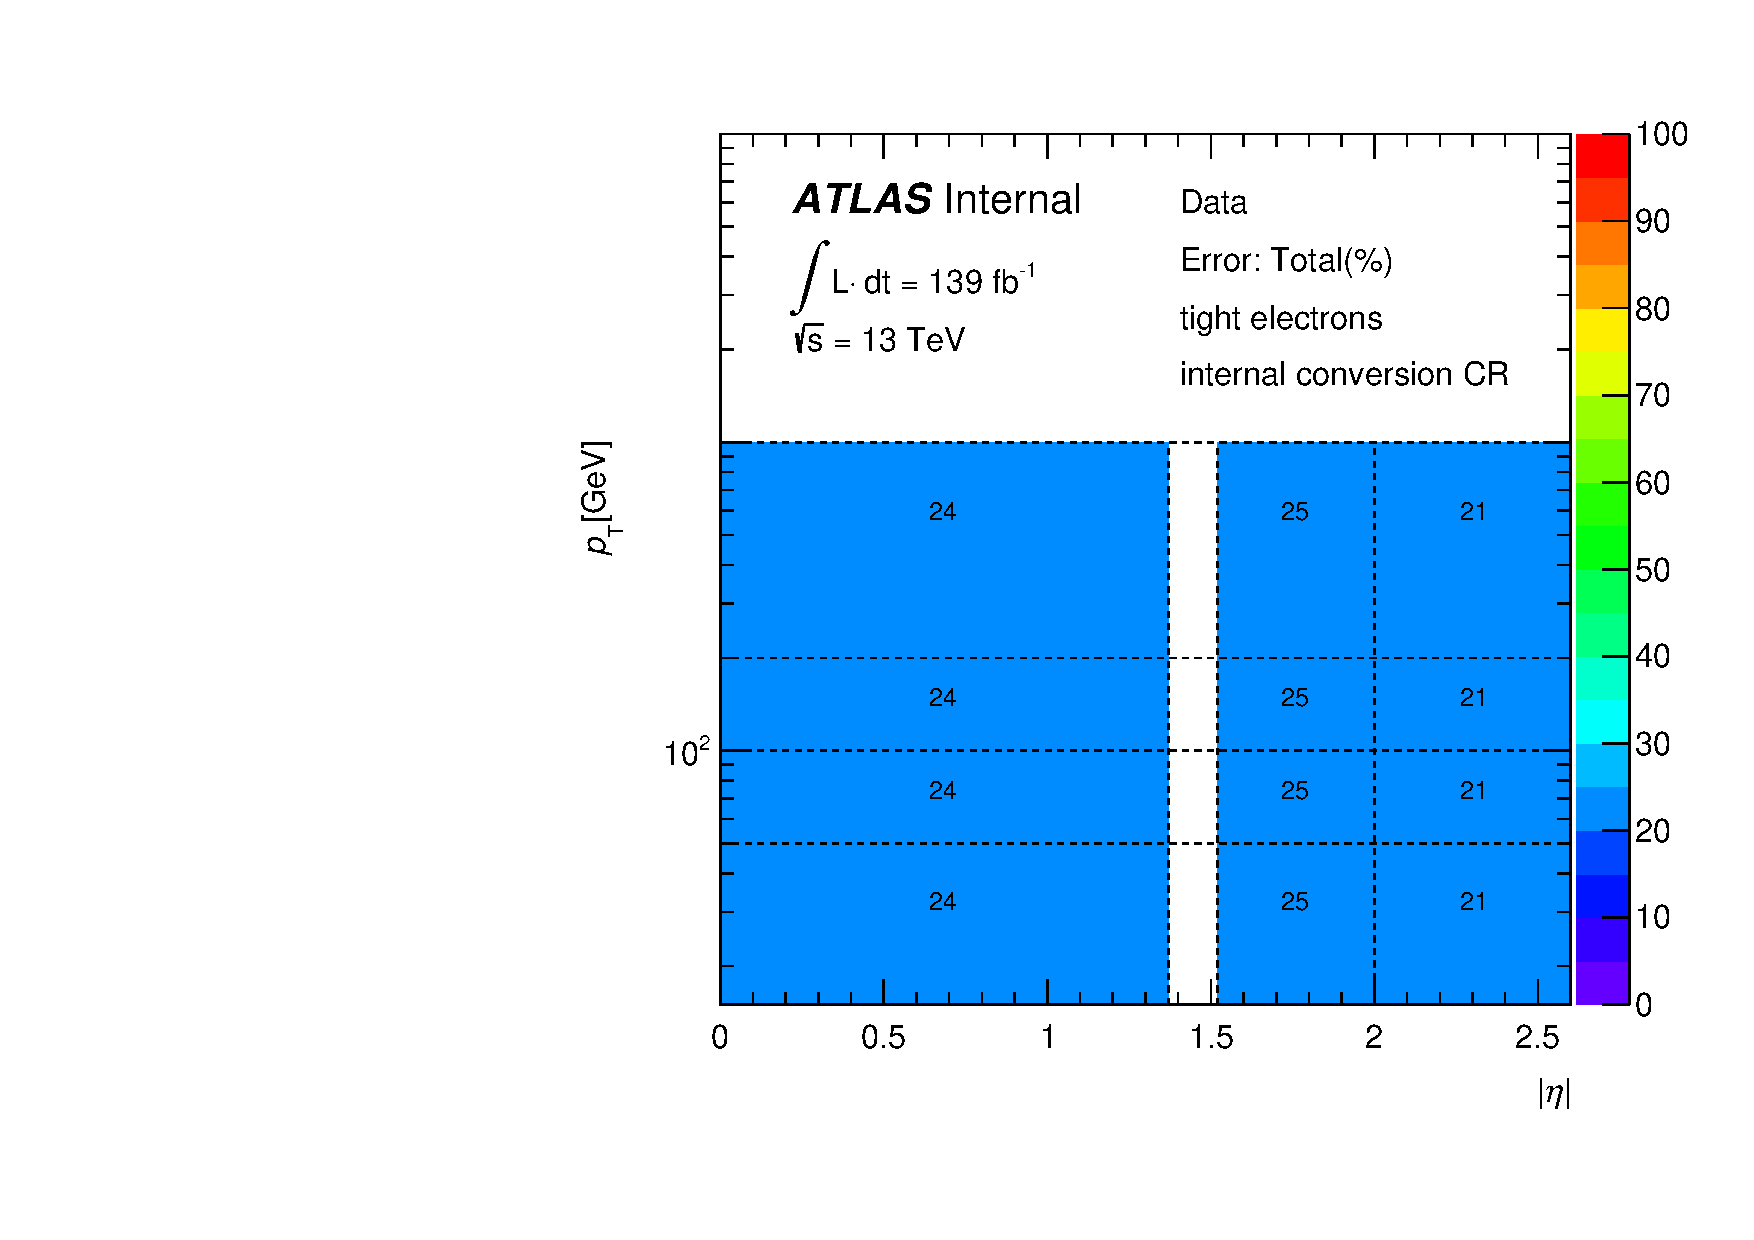
\includegraphics[width=0.45\textwidth]{figures/qmisid/syst_Data_Total_tight_intcr}\\
  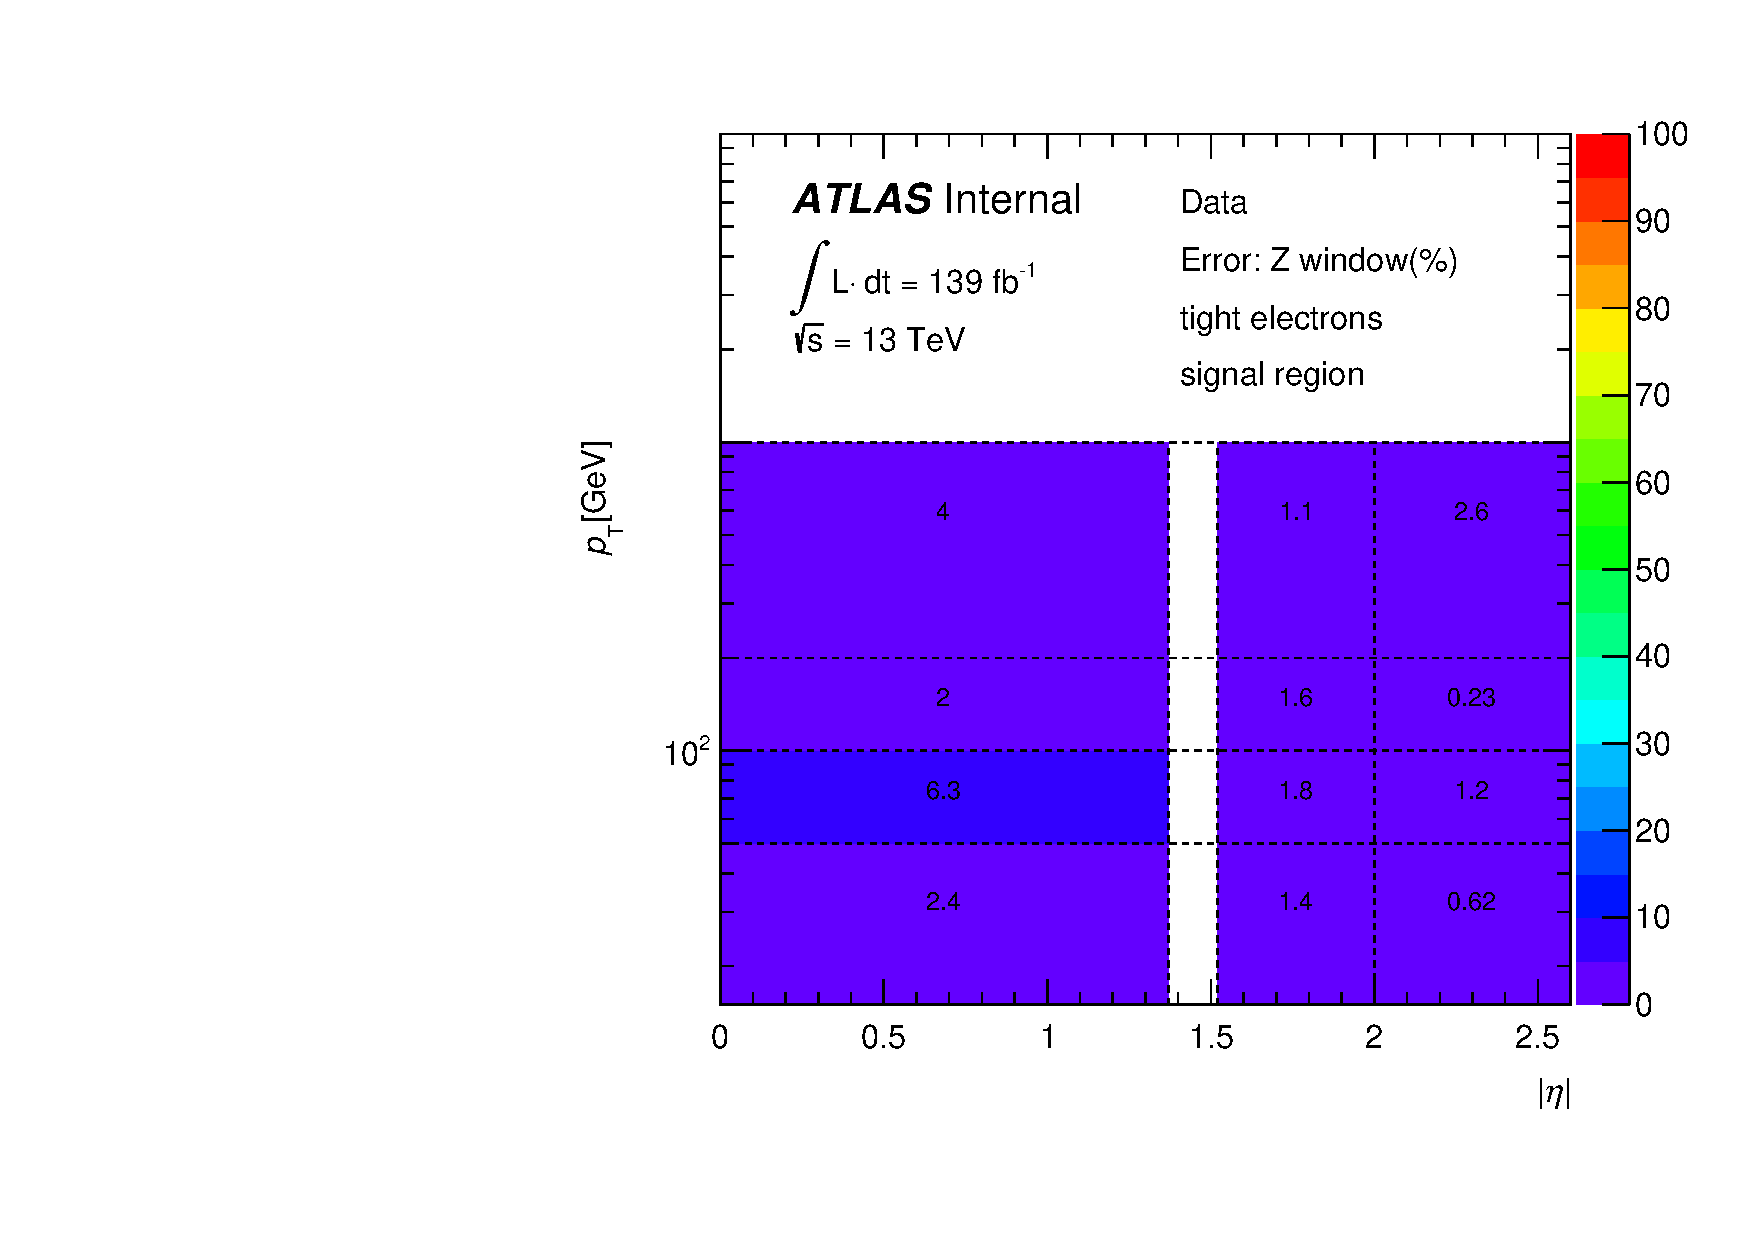
\includegraphics[width=0.45\textwidth]{figures/qmisid/syst_Data_Zwindow_tight_sr}
  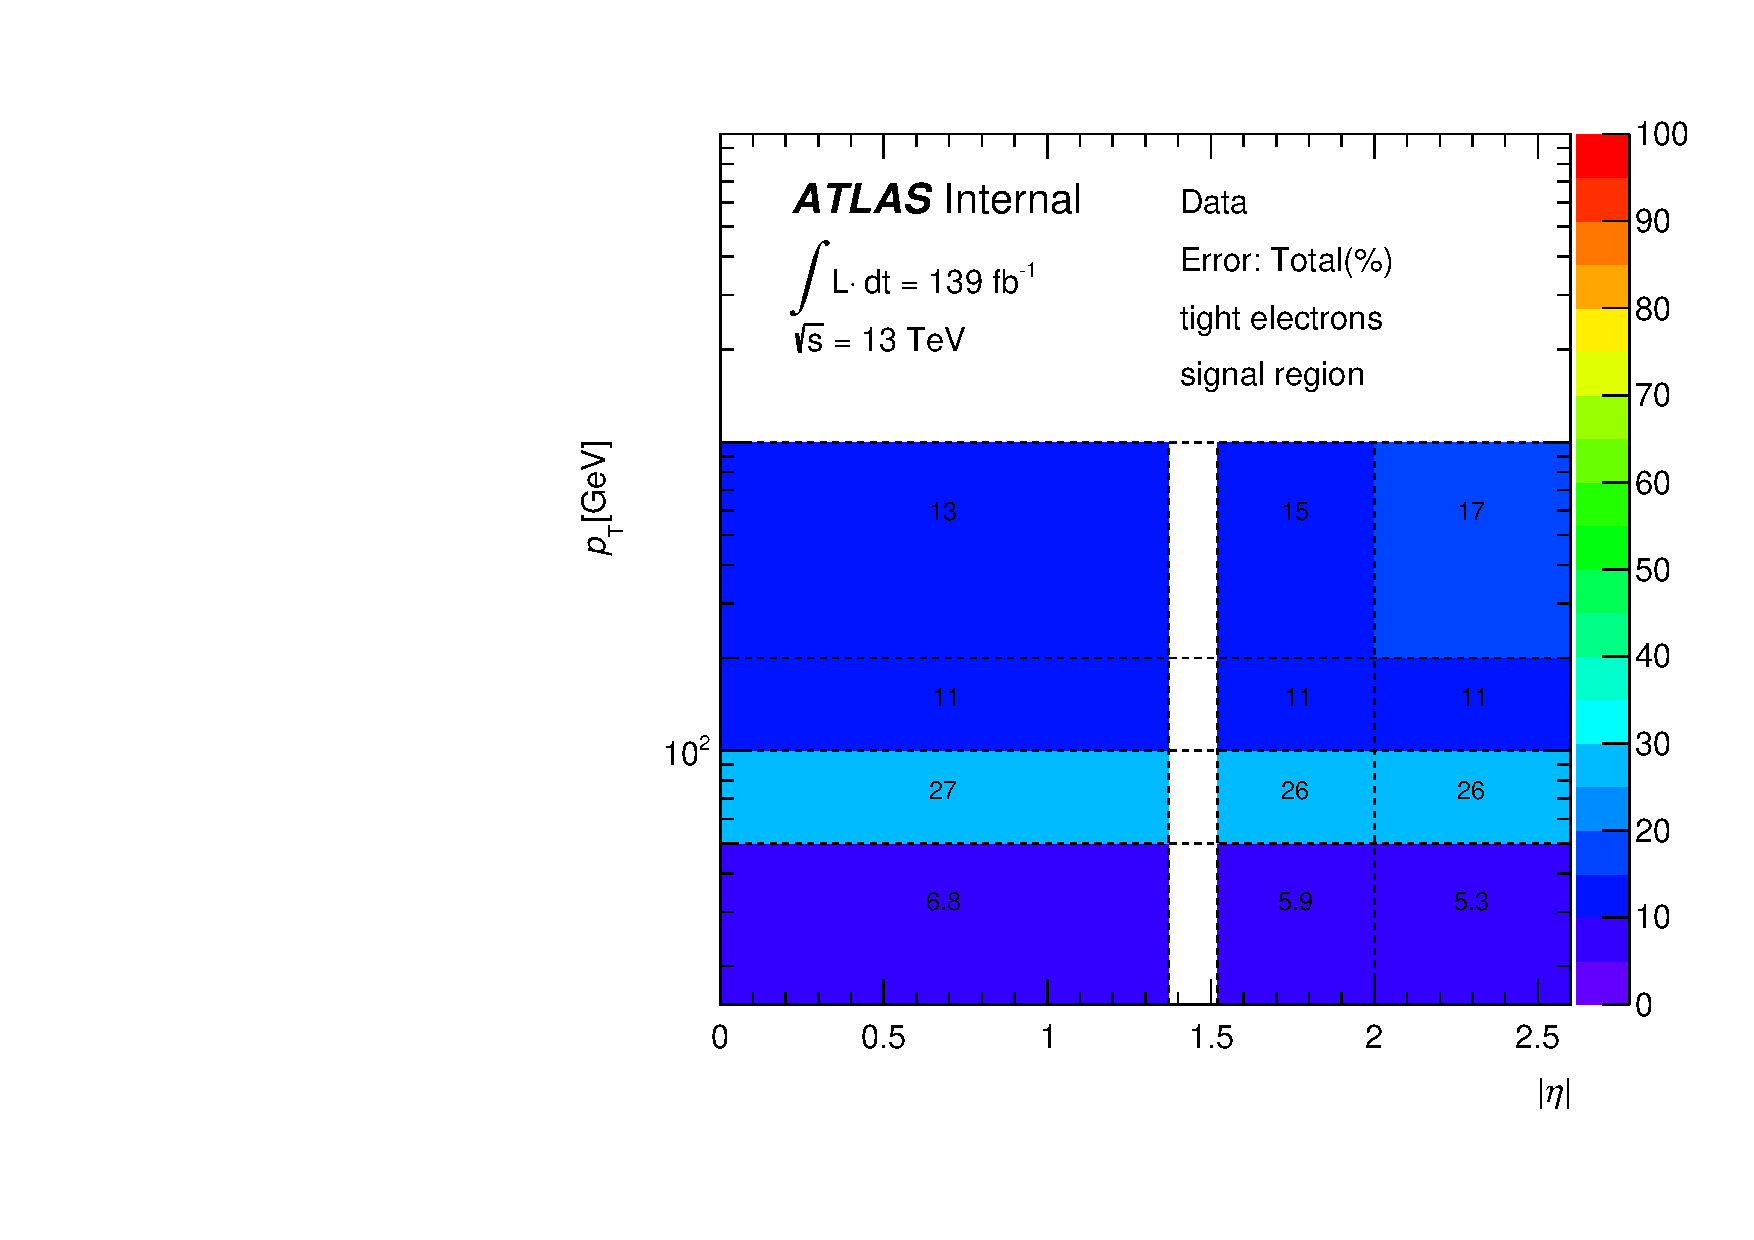
\includegraphics[width=0.45\textwidth]{figures/qmisid/syst_Data_Total_tight_sr}
  \caption{ \label{fig:QMisID:systb} Left: systematic uncertainty (\%), introduced from the variation of the $m_{Z}$ window
  (and its sidebands) that is used to obtain the rates, in bins of $|\eta|$ and $\pT$. Right: Total systematic uncertainty (\%).}
  \end{center}
\end{figure}

%~~~~~~~~~~~~~~~~~~~~~~~~~~~~~~~~~~~
\subsubsection{Closure test}
\label{Sec:closure}
%~~~~~~~~~~~~~~~~~~~~~~~~~~~~~~~~~~~

The rates are validated by comparing the estimated number of same-sign $ee$ events (using the QMisID rates on
opposite-sign events) to the measured number of same-sign events. In order to increase the statistical
precision, this test is performed without any requirement regarding the number of jets. 
Figure\,\ref{fig:clData}, shows the expected distribution of $m_{ee}$ in the data, compared to the observation
(the latter also contains contributions from non-prompt electrons). 
After subtracting the non-prompt electron background using the sidebands, the
measured number of same-sign events in the $m_{Z}$ window is found to be 6474
(1076) for events with at least 1 jet (3 jets) while the expectation is
$6951 \pm 1024$ ($1156 \pm 95$). The $\pT$ distribution (within the $m_{Z}$ window) is also presented 
in figure\,\ref{fig:clData}, showing agreement between the measurement and the prediction, which however begins 
to deteriorate in the very high $\pT$ region, due to the fact that the region above 200\,GeV is described by an 
inclusive QmisID rate.

The respective comparison with $Z$+jets MC (in which the non-prompt contribution is removed using the truth 
information) is shown in figure\,\ref{fig:clMC}.

\begin{figure}[htb!]
\centering
  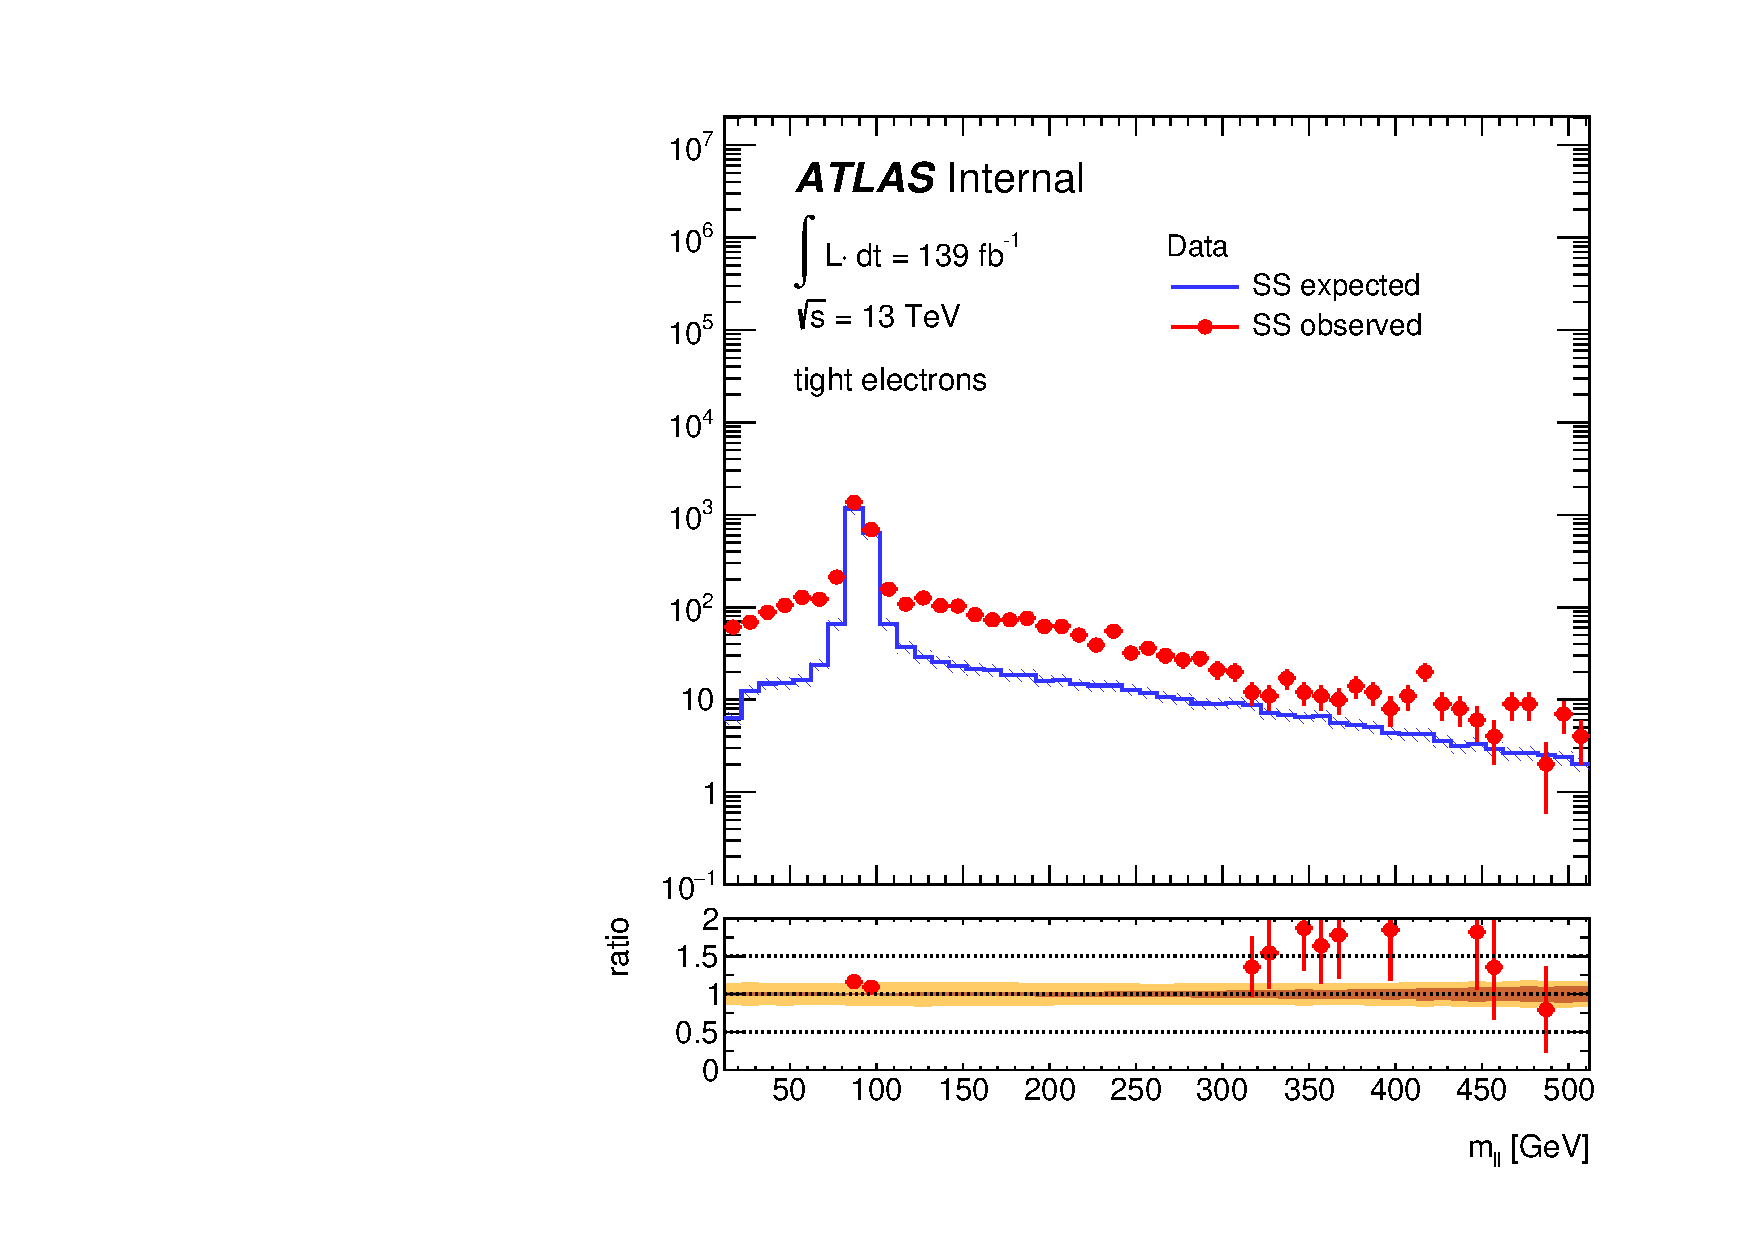
\includegraphics[width=0.45\textwidth]{figures/qmisid/valid_MlltightData}
  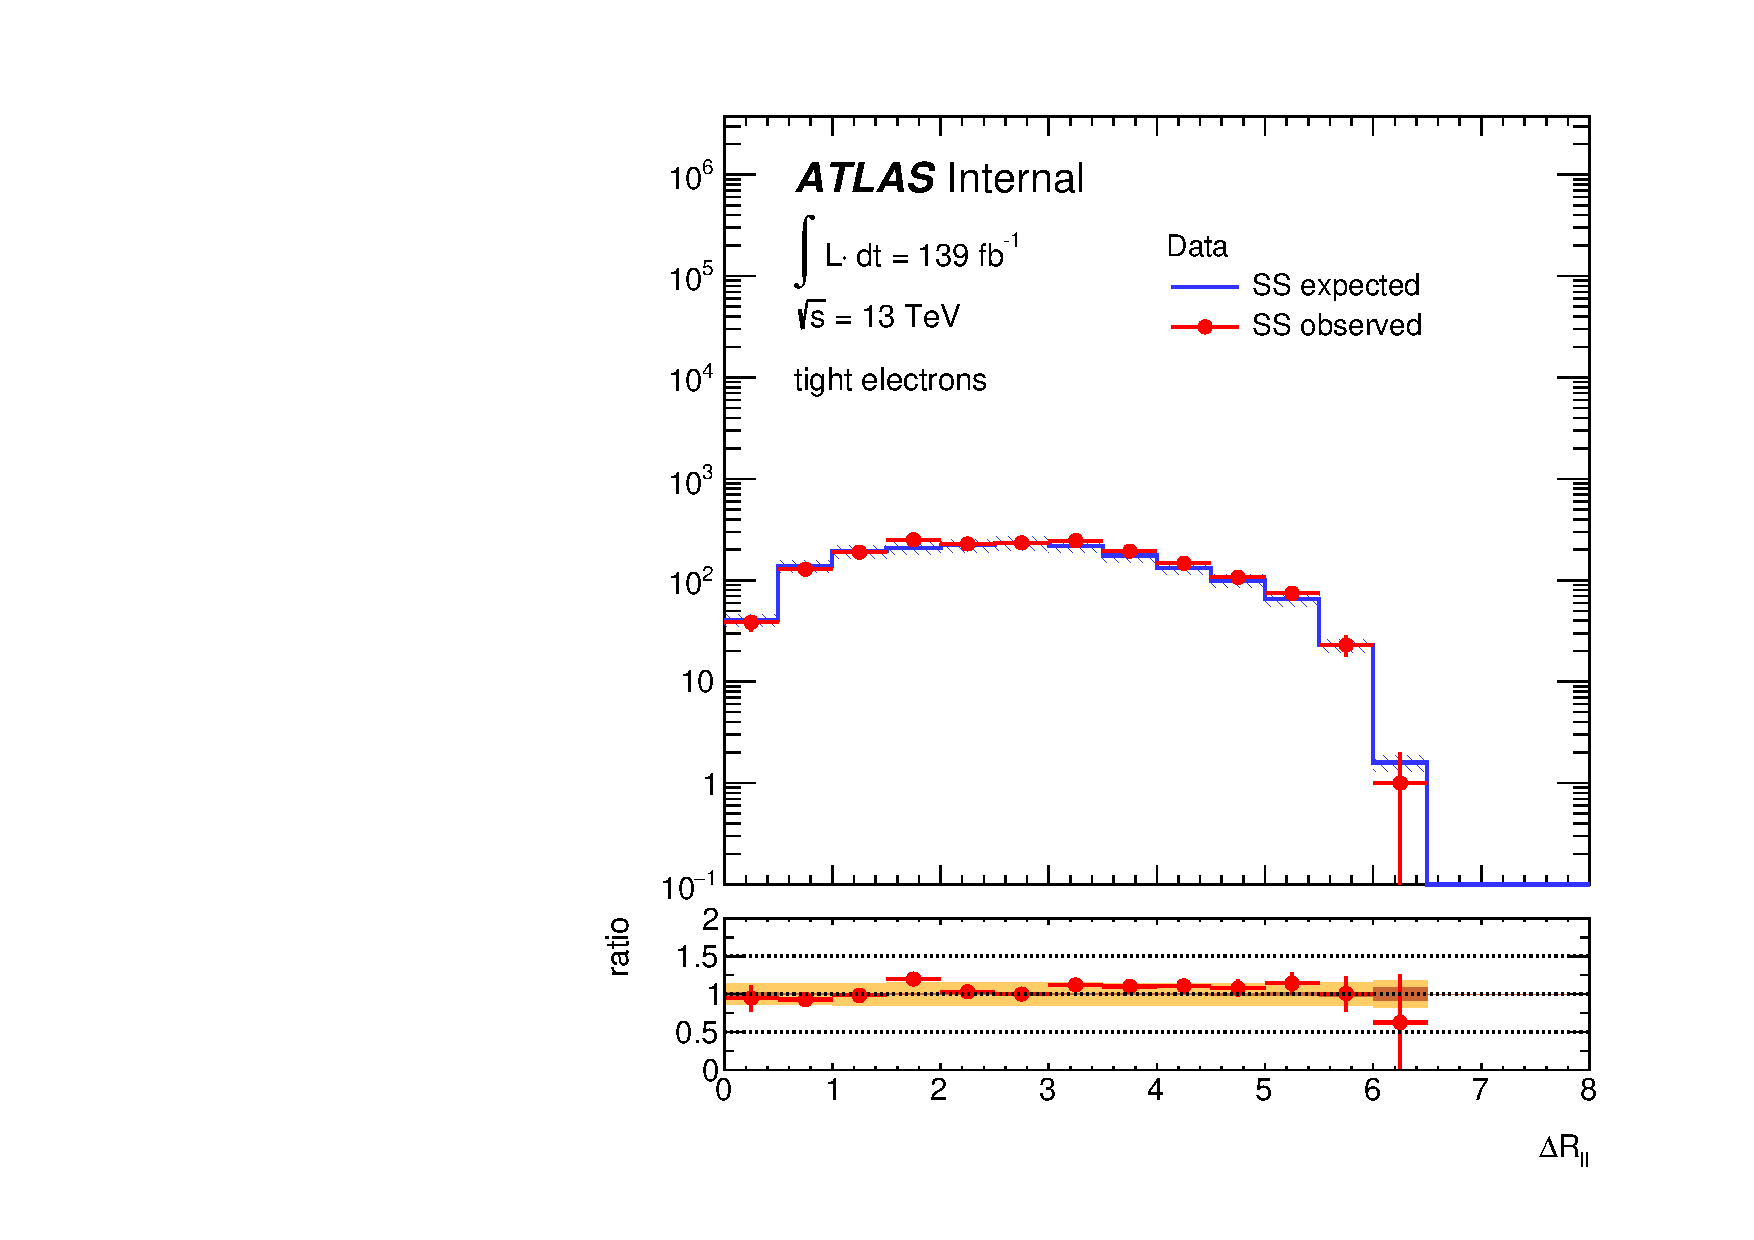
\includegraphics[width=0.45\textwidth]{figures/qmisid/valid_DRlltightData}\\
  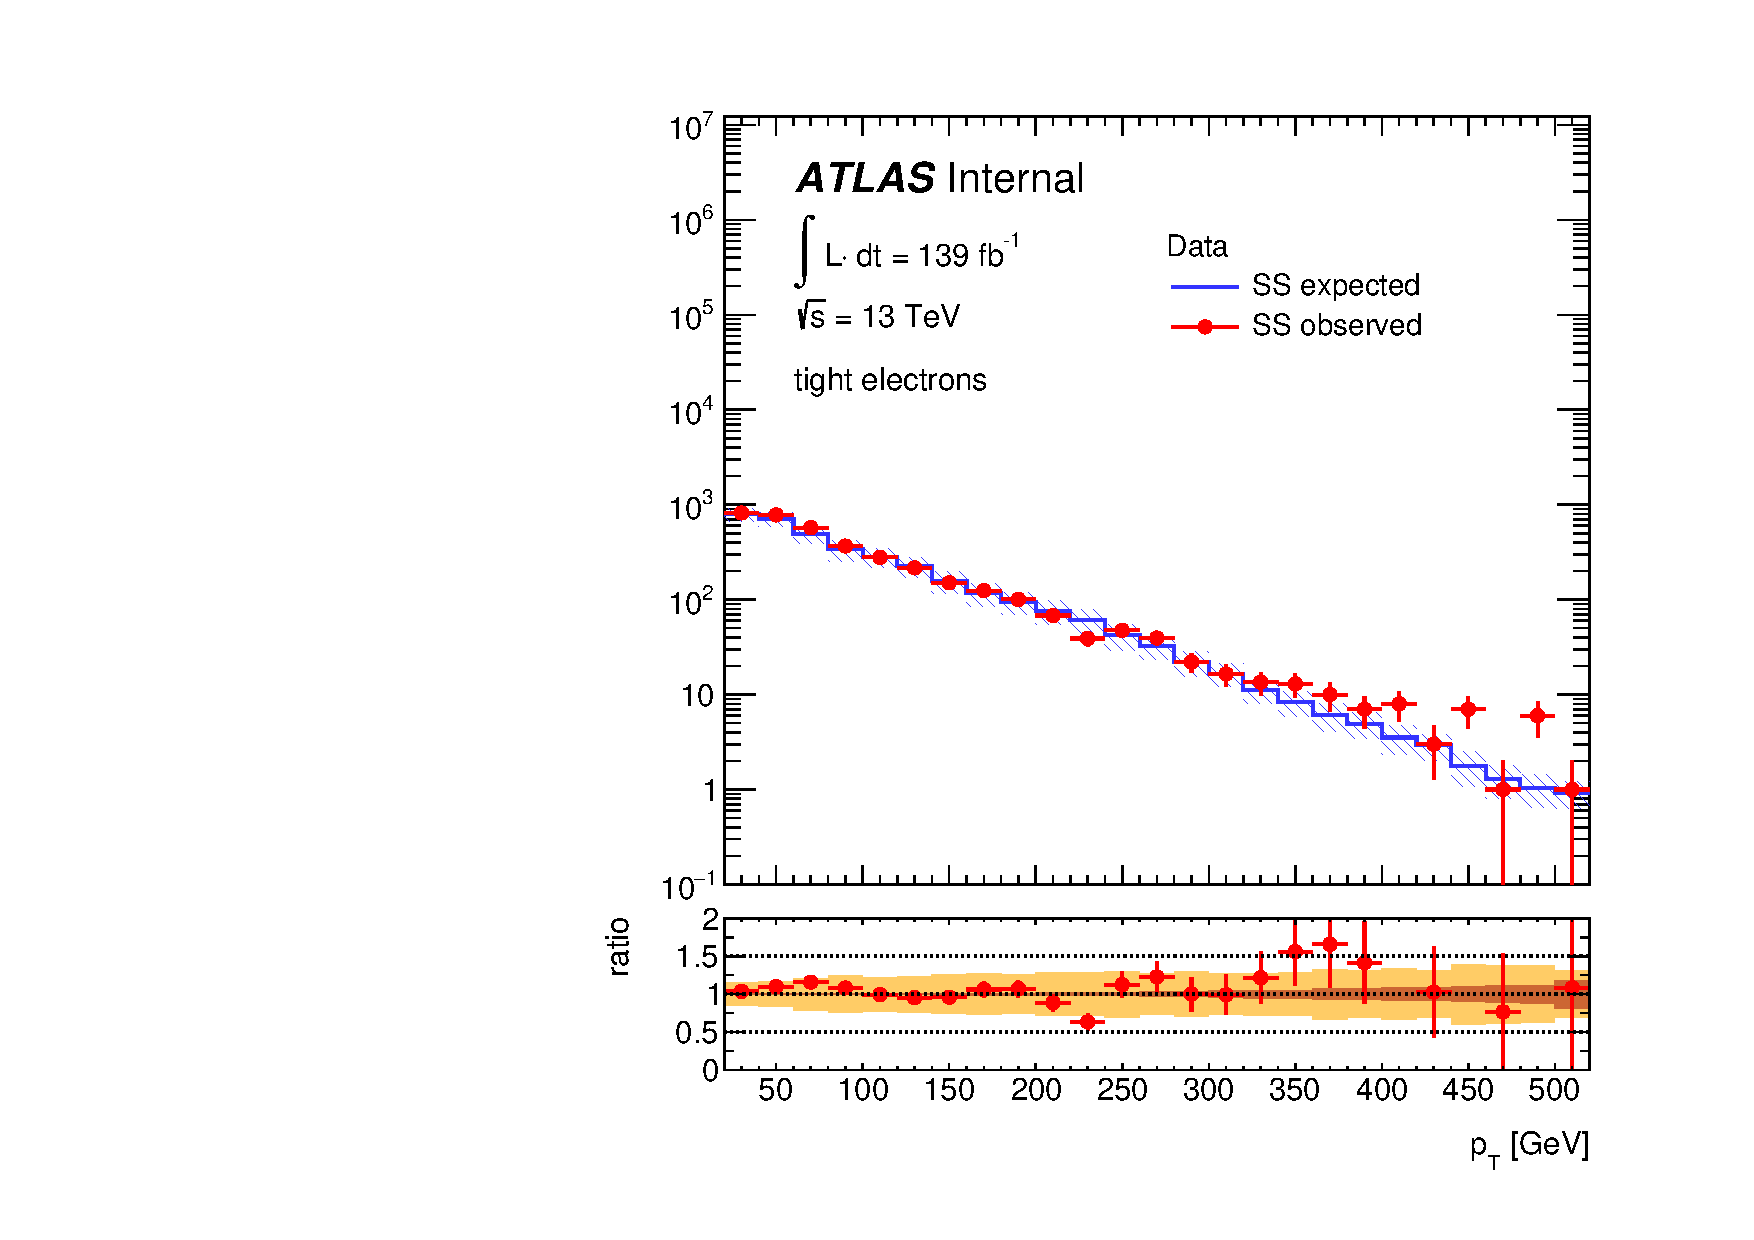
\includegraphics[width=0.45\textwidth]{figures/qmisid/valid_PttightData}
  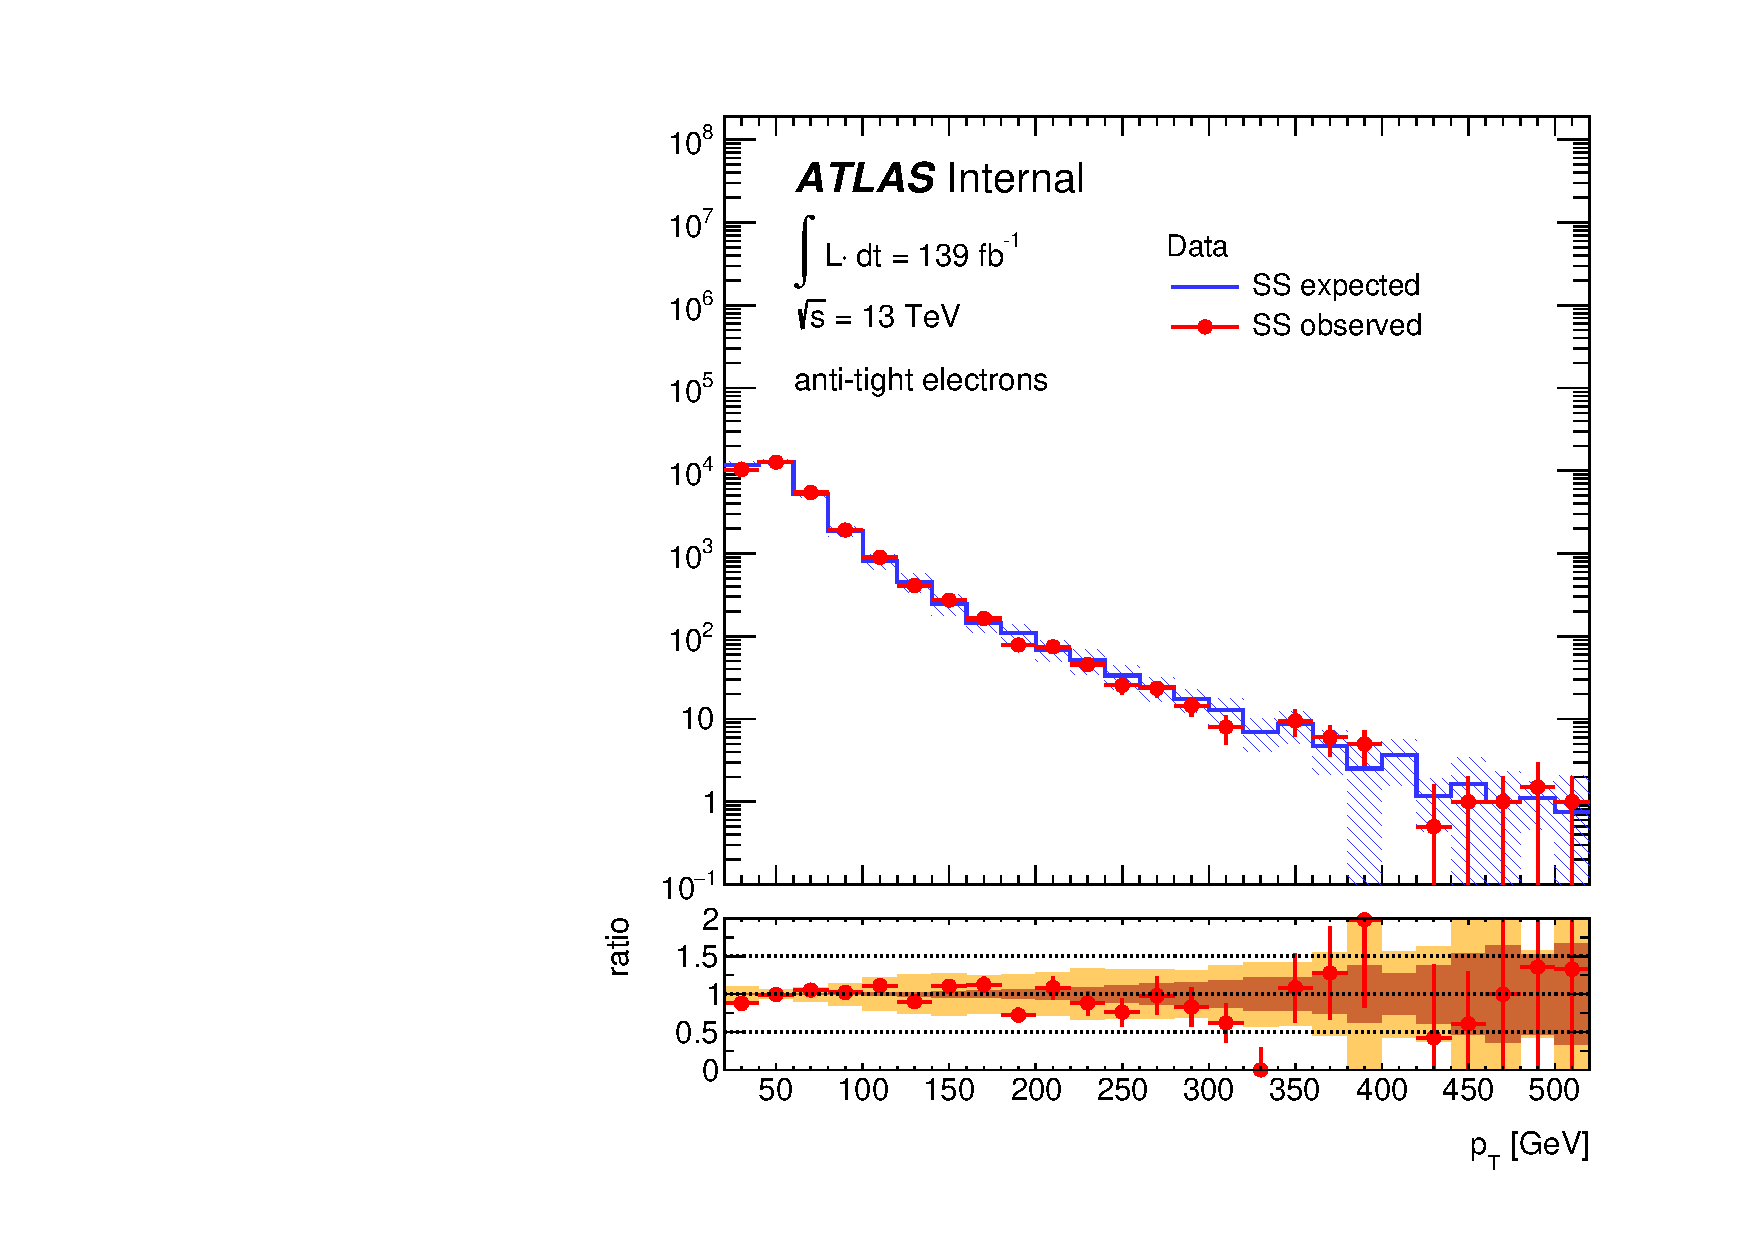
\includegraphics[width=0.45\textwidth]{figures/qmisid/valid_PtatightData}\\
  \caption{Comparison between the expected and observed $m_{ee}$, ${\Delta}R_{ee}$, $pT$ (tight) and $\pT$ (anti-tight) of same-sign electrons.  The dashed bands represent the total (statistical + systematic) uncertainty of the estimation. The comparison is shown for data events. The observed $m_{ee}$ distribution includes the contribution of fake electrons, which are later subtracted by using the sidebands.\label{fig:clData}}
\end{figure}


\begin{figure}[htb!]
\centering
  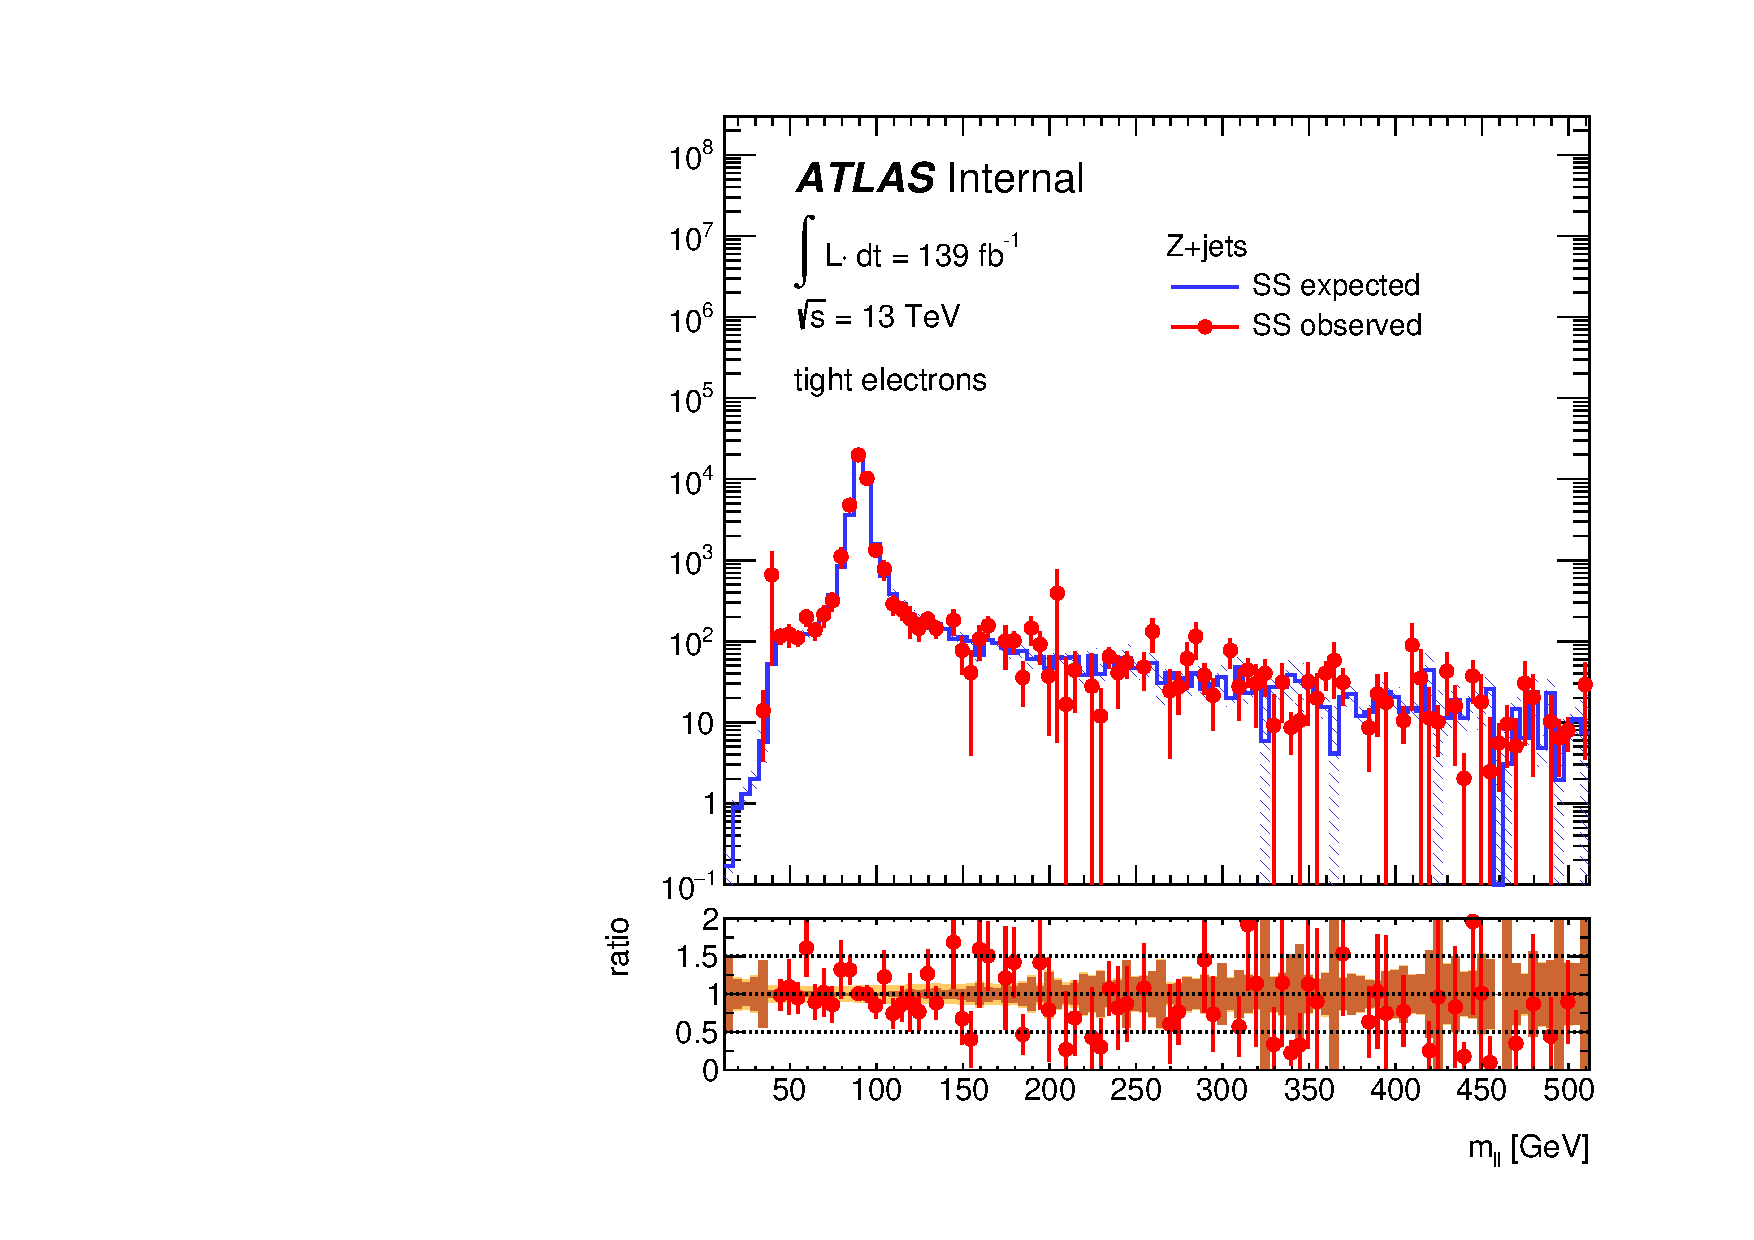
\includegraphics[width=0.45\textwidth]{figures/qmisid/valid_MlltightZ}
  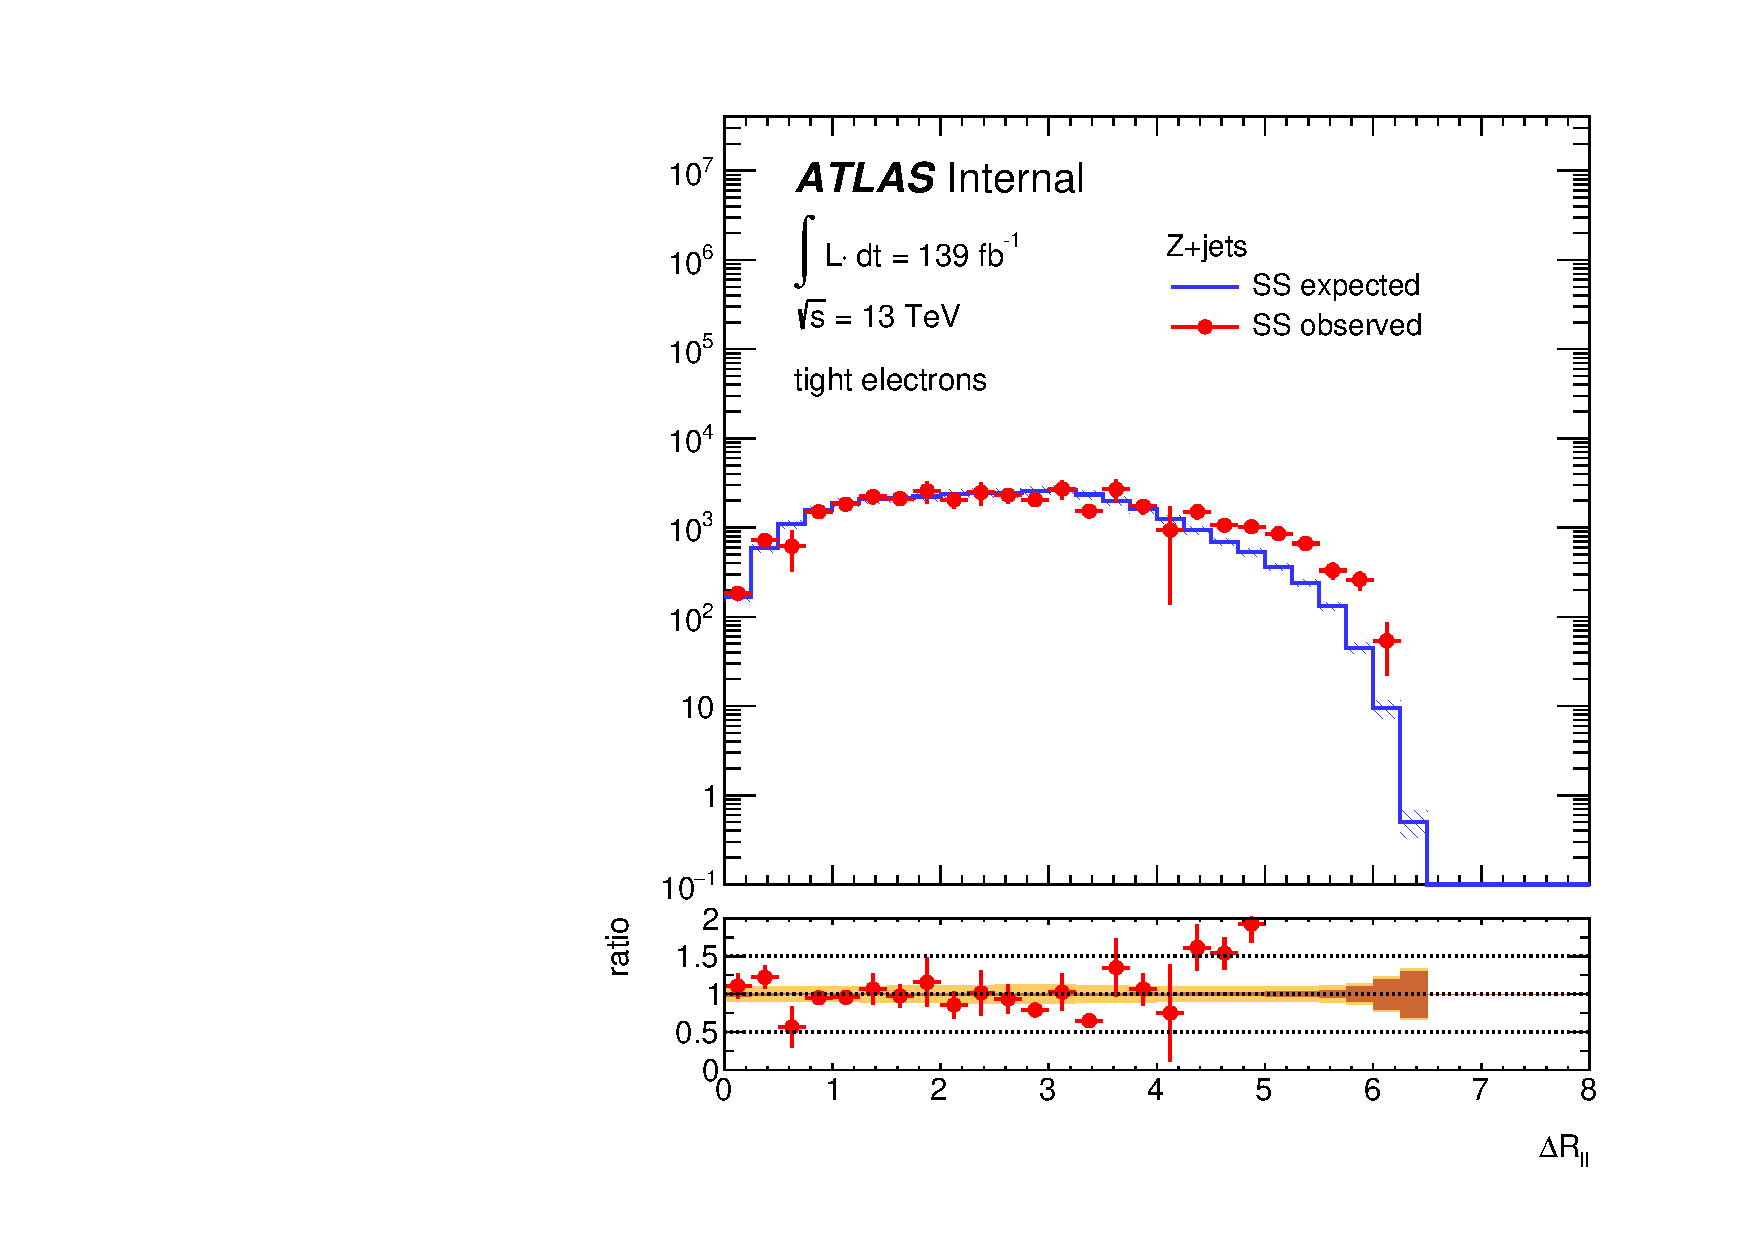
\includegraphics[width=0.45\textwidth]{figures/qmisid/valid_DRlltightZ}\\
  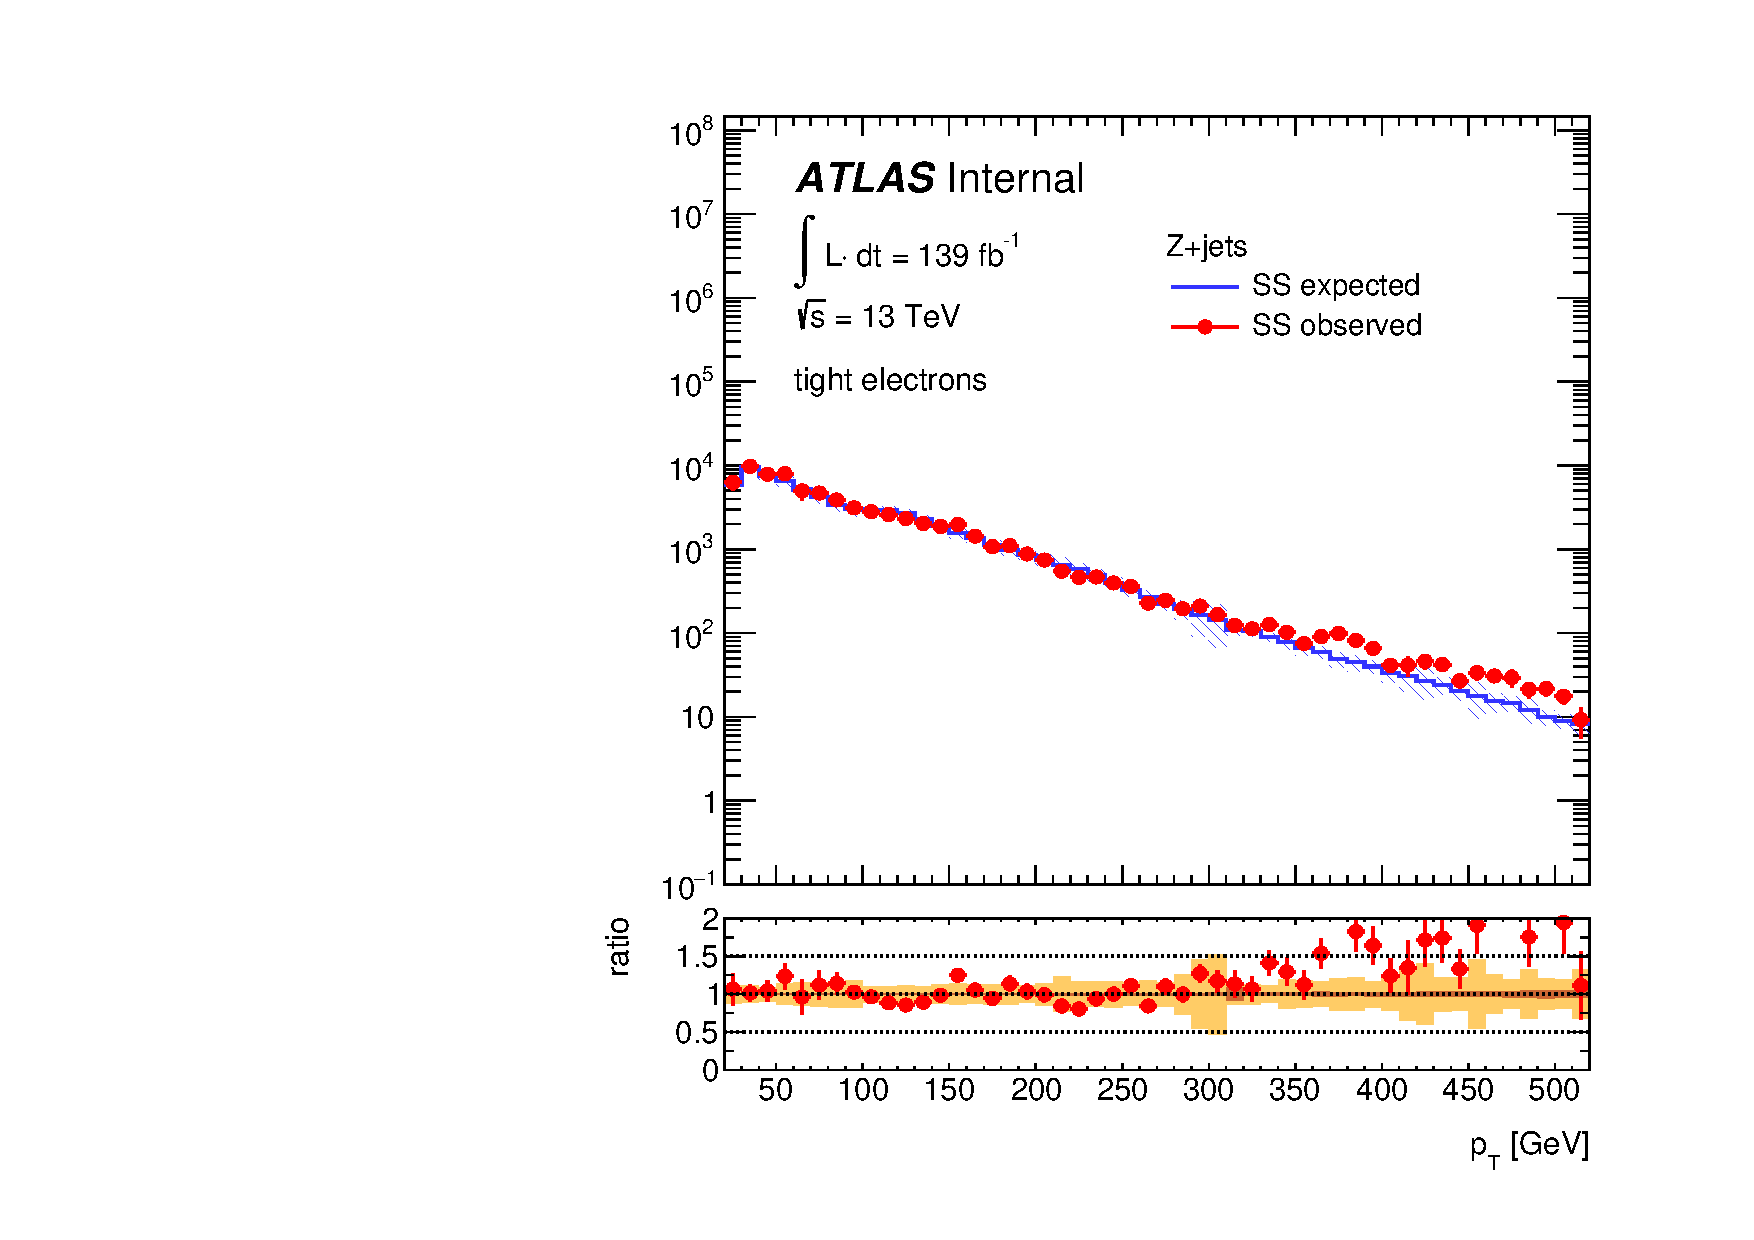
\includegraphics[width=0.45\textwidth]{figures/qmisid/valid_PttightZ}
  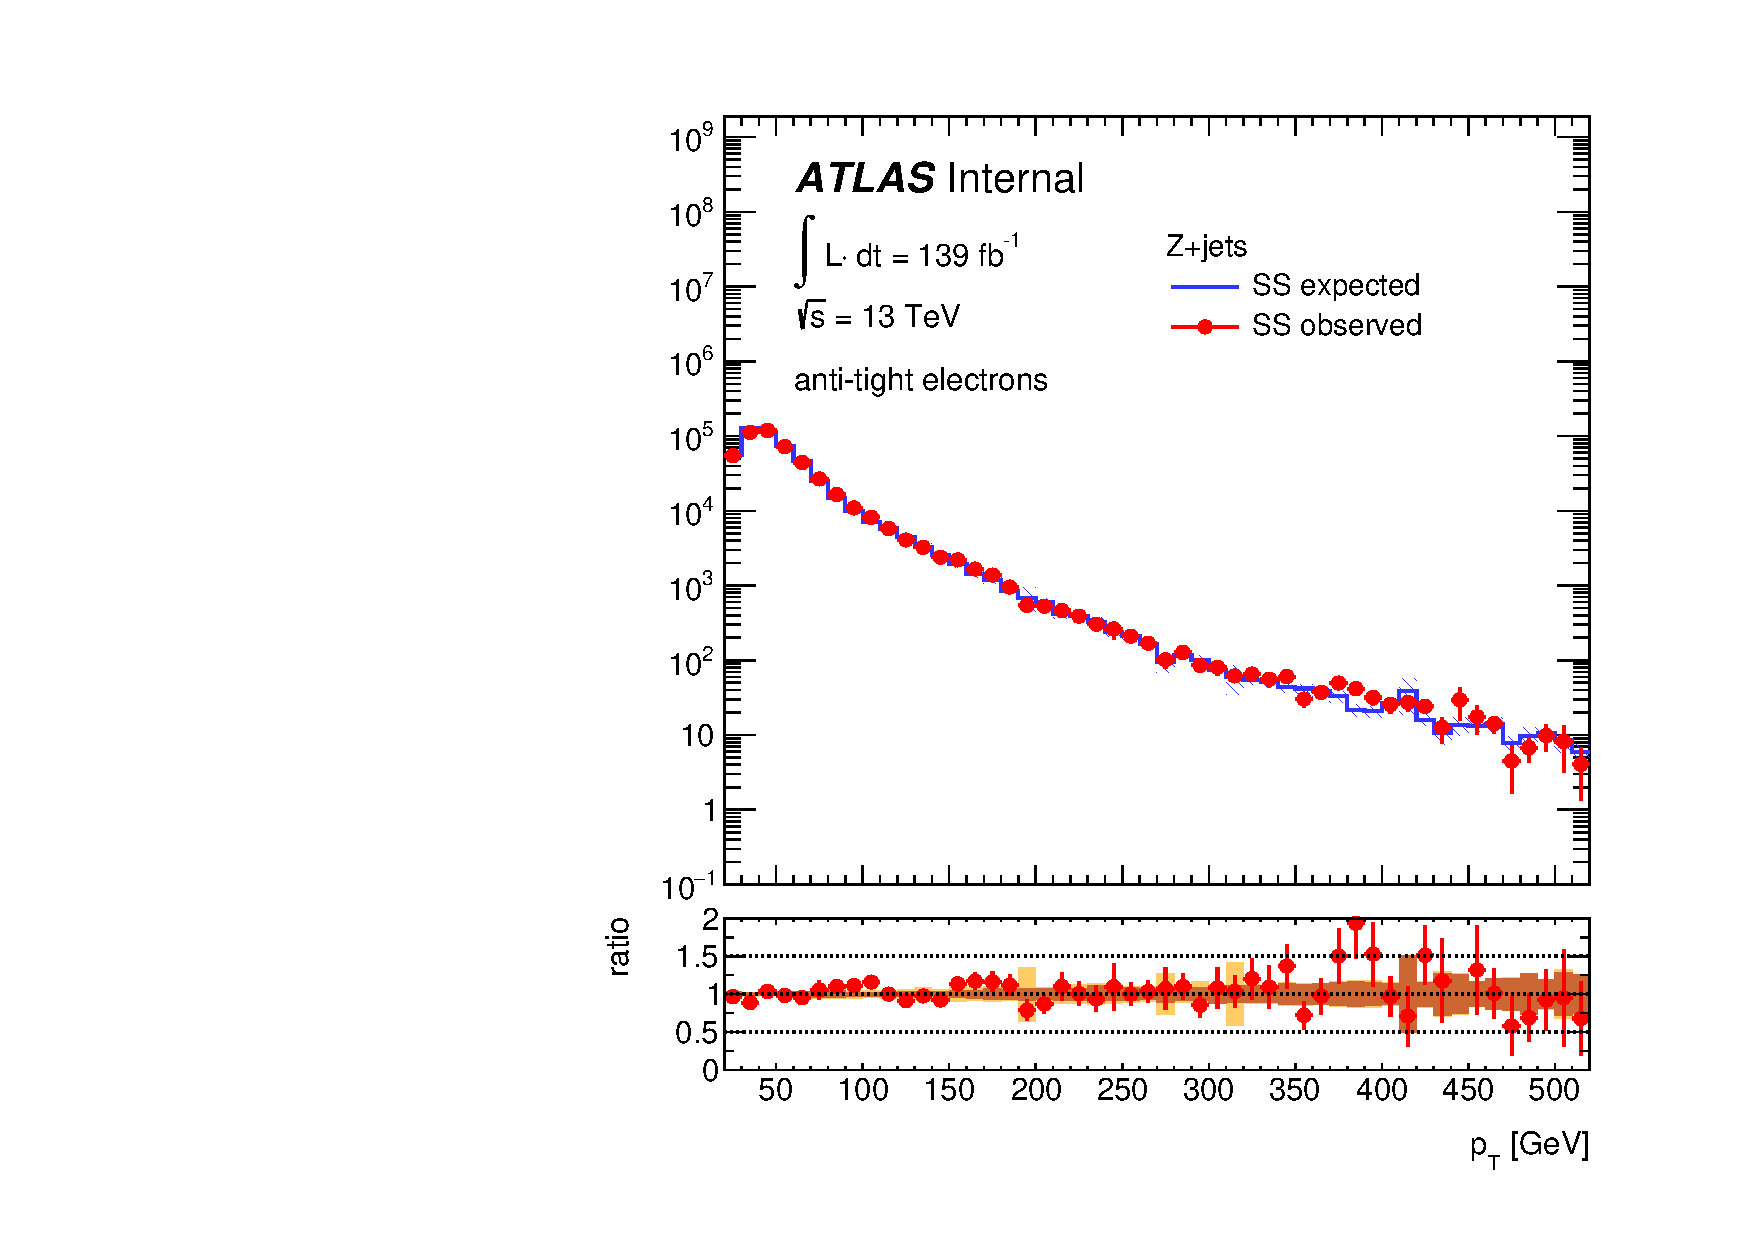
\includegraphics[width=0.45\textwidth]{figures/qmisid/valid_PtatightZ}\\
  \caption{Comparison between the expected and observed $m_{ee}$,
${\Delta}R_{ee}$, $\pT$ (tight) and $\pT$ (anti-tight) of same-sign electrons.
The dashed bands represent the total (statistical + systematic) uncertainty of the estimation.
 The comparison is shown for $Z$+jets events. Fake electrons are removed from
 the sample by using the truth information.\label{fig:clMC}} 
\end{figure}

